\documentclass [11pt,twoside]{article}
\usepackage[utf8]{inputenc}
\usepackage[T1]{fontenc}
\usepackage{xltabular}
\usepackage{booktabs} 
\usepackage{graphicx}


%Page margins, header and footer positions
\usepackage{geometry}
\geometry{
 a4paper,
 total={210mm,297mm},
 left=25mm,
 right=25mm,
 top=30mm,
 bottom=25mm,
 headsep=7mm}

\interfootnotelinepenalty=10000

%To display filling dots in the TOC for all entries
\usepackage[titles]{tocloft}
\renewcommand{\cftsecleader}{\cftdotfill{\cftdotsep}}

%Define new header and footer style
\usepackage{fancyhdr}

\pagestyle{fancy}
\fancyhf{}
%\lhead{\color{Gray}{\small{Travlendar+ project by YOUR NAMES}}}
\lfoot{\textcolor{Gray}{\small{Copyright © 2024, D. Motiallah, S. Chaudhury, D. Islam – All rights reserved}}}
\rfoot{\textcolor{Gray}{\thepage}}
\renewcommand{\headrulewidth}{0pt}

%PACKAGES
\usepackage{wasysym}
\usepackage{pifont}
\usepackage{placeins}
\usepackage{array}
\usepackage{graphicx}


\newcommand{\supported}{\ding{52}\xspace}
\newcommand{\unsupported}{\ding{55}\xspace}
\newcommand{\partsupported}{\textcolor{black!40}{\ding{52}}\xspace}
\newcommand{\lowsupported}{\textcolor{black!20}{\ding{52}}\xspace}
\newcommand{\unknowsupported}{\textbf{?}\xspace}

%Font: Times
\usepackage{times}
%Change monospaced font
\renewcommand{\ttdefault}{lmtt}

%tables
\usepackage{tabu}
\usepackage{tabularx}
\usepackage{ltablex}
\usepackage{longtable}
\usepackage{float} % To allow the use of H modifier in long tables

%landscape mode
\usepackage{pdflscape}
\usepackage{rotating}
\usepackage{caption}

%make landscape mode be sensitive to even and odd pages
%start
\def\myrotate{\ifodd\c@page\else-\fi 90}
\makeatletter
\global\let\orig@begin@landscape=\landscape%
\global\let\orig@end@landscape=\endlandscape%
\gdef\@true{1}
\gdef\@false{0}
\gdef\landscape{%
    \global\let\within@landscape=\@true%
    \orig@begin@landscape%
}%
\gdef\endlandscape{%
    \orig@end@landscape%
    \global\let\within@landscape=\@false%
}%
\@ifpackageloaded{pdflscape}{%
    \gdef\pdf@landscape@rotate{\PLS@Rotate}%
}{
    \gdef\pdf@landscape@rotate#1{}%
}
\let\latex@outputpage\@outputpage
\def\@outputpage{
    \ifx\within@landscape\@true%
        \if@twoside%
            \ifodd\c@page%
                \gdef\LS@rot{\setbox\@outputbox\vbox{%
                    \pdf@landscape@rotate{-90}%
                    \hbox{\rotatebox{90}{\hbox{\rotatebox{180}{\box\@outputbox}}}}}%
                }%
            \else%
                \gdef\LS@rot{\setbox\@outputbox\vbox{%
                    \pdf@landscape@rotate{+90}%
                    \hbox{\rotatebox{90}{\hbox{\rotatebox{0}{\box\@outputbox}}}}}%
                }%
            \fi%
        \else%
            \gdef\LS@rot{\setbox\@outputbox\vbox{%
                \pdf@landscape@rotate{+90}%
                \hbox{\rotatebox{90}{\hbox{\rotatebox{0}{\box\@outputbox}}}}}%
            }%
        \fi%
    \fi%
    \latex@outputpage%
}
\makeatother
%end

%graphics
\usepackage{graphicx}
\usepackage[dvipsnames, table]{xcolor}
%If you upload images from PC, you need to insert code for the path here (different for Windows and Unix OS)

%References
%\usepackage{xpatch}
%\usepackage[backend=biber, style=numeric, citestyle=numeric, sorting=none]{biblatex}
%\addbibresource{main.bib}

%Other
\usepackage{ifthen}
\usepackage{xspace}
\usepackage{enumitem}
\usepackage{amssymb}
\usepackage[pdftex, colorlinks]{hyperref}
\newcommand{\comment}[1]{{\color{Red}$\blacktriangleright$ Comment: #1 $\blacktriangleleft$}}


% Some utilities\ldots
\usepackage{soul}
\usepackage{tikz}

\usetikzlibrary{calc}
\usetikzlibrary{decorations.pathmorphing}


\makeatletter

\newcommand{\defhighlighter}[3][]{%
  \tikzset{every highlighter/.style={color=#2, fill opacity=#3, #1}}%
}

\defhighlighter{yellow}{.5}

\newcommand{\highlight@DoHighlight}{
  \fill [ decoration = {random steps, amplitude=1pt, segment length=15pt}
        , outer sep = -15pt, inner sep = 0pt, decorate
       , every highlighter, this highlighter ]
        ($(begin highlight)+(0,8pt)$) rectangle ($(end highlight)+(0,-3pt)$) ;
}

\newcommand{\highlight@BeginHighlight}{
  \coordinate (begin highlight) at (0,0) ;
}

\newcommand{\highlight@EndHighlight}{
  \coordinate (end highlight) at (0,0) ;
}

\newdimen\highlight@previous
\newdimen\highlight@current

\DeclareRobustCommand*\highlight[1][]{%
  \tikzset{this highlighter/.style={#1}}%
  \SOUL@setup
  %
  \def\SOUL@preamble{%
    \begin{tikzpicture}[overlay, remember picture]
      \highlight@BeginHighlight
      \highlight@EndHighlight
    \end{tikzpicture}%
  }%
  %
  \def\SOUL@postamble{%
    \begin{tikzpicture}[overlay, remember picture]
      \highlight@EndHighlight
      \highlight@DoHighlight
    \end{tikzpicture}%
  }%
  %
  \def\SOUL@everyhyphen{%
    \discretionary{%
      \SOUL@setkern\SOUL@hyphkern
      \SOUL@sethyphenchar
      \tikz[overlay, remember picture] \highlight@EndHighlight ;%
    }{%
    }{%
      \SOUL@setkern\SOUL@charkern
    }%
  }%
  %
  \def\SOUL@everyexhyphen##1{%
    \SOUL@setkern\SOUL@hyphkern
    \hbox{##1}%
    \discretionary{%
      \tikz[overlay, remember picture] \highlight@EndHighlight ;%
    }{%
    }{%
      \SOUL@setkern\SOUL@charkern
    }%
  }%
  %
  \def\SOUL@everysyllable{%
    \begin{tikzpicture}[overlay, remember picture]
      \path let \p0 = (begin highlight), \p1 = (0,0) in \pgfextra
        \global\highlight@previous=\y0
        \global\highlight@current =\y1
      \endpgfextra (0,0) ;
      \ifdim\highlight@current < \highlight@previous
        \highlight@DoHighlight
        \highlight@BeginHighlight
      \fi
    \end{tikzpicture}%
    \the\SOUL@syllable
    \tikz[overlay, remember picture] \highlight@EndHighlight ;%
  }%
  \SOUL@
}

\makeatother

% Common abbrev. are set as commands to ensure proper spacing after the dot
\RequirePackage{xspace}
\newcommand{\ie}{i.e.\@\xspace}
\newcommand{\aka}{a.k.a.\@\xspace}
\newcommand{\Ie}{I.e.\@\xspace}
\newcommand{\cf}{cf.\@\xspace}
\newcommand{\Cf}{Cf.\@\xspace}
\newcommand{\eg}{e.g.\@\xspace}
\newcommand{\Eg}{E.g.\@\xspace}
\newcommand{\etal}{et al.\@\xspace}
\newcommand{\etc}{etc.\@\xspace}
\newcommand{\wrt}{w.r.t.\@\xspace}
\newcommand{\Wrt}{W.r.t.\@\xspace}



\date{}

\begin{document}

%TITLE PAGE

\begin{titlepage}


%LOGO

\begin{table}[t!]
\centering
\begin{tabu} to \textwidth { X[1.3,r,p] X[1.7,l,p] }
\textcolor{Blue}
%{\textbf{\small{Travlendar+ project YOUR NAMES}}} 
&

\includegraphics[scale=0.5]{Images/PolimiLogo}
\end{tabu}
\end{table}

%TITLE 

\begin{flushleft}

%Replace the text string with your title
{\textcolor{Blue}{\textbf{\Huge{Design Document}}}} \\ [1cm]

\end{flushleft}

%Define deliverable specific info
%Replace cell contents where needed
\begin{table}[h!]
\begin{tabu} to \textwidth { X[0.3,r,p] X[0.7,l,p] }
\hline
\\
\textbf{Deliverable:} & DD\\
\textbf{Title:} & Design Document\\
\textbf{Authors:} & Dorsa Motiallah, Sujata Chaudhury, Darkhan Islam \\
\textbf{Version:} & 1.0 \\ 
\textbf{Date:} & 07-January-2025 \\
\textbf{Download page:} & https://github.com/dorsamotiallah/MotiallahChaudhuryIslam \\
\textbf{Copyright:} & Copyright © 2024, D. Motiallah, S. Chaudhury, D. Islam – All rights reserved \\ \\

\hline
\end{tabu}
\end{table}

\end{titlepage}






\setcounter{page}{2}


%------------------------------------------------------------------------------------------------------------------------------------------------
\newpage
\addcontentsline{toc}{section}{Table of Contents}
\tableofcontents
\newpage
\addcontentsline{toc}{section}{List of Figures}
\listoffigures
\addcontentsline{toc}{section}{List of Tables}
\listoftables

%------------------------------------------------------------------------------------------------------------------------------------------------
\clearpage
{\section{Introduction}
\label{sect:introduction}
\subsection{Purpose}
The purpose of the Students \& Companies (S\&C) project is to create a platform that efficiently matches university students with suitable internship opportunities based on their skills, experiences, and preferences, while also meeting the needs of companies seeking to recruit talent. The platform streamlines the entire internship process, from profile creation and internship listings to matching, interview management, and feedback collection. It aims to improve the overall internship experience, enhance the selection process, and provide universities with tools to monitor and ensure the quality of internships, ultimately benefiting students, companies, and academic institutions alike.
\newline The S\&C platform creates a dynamic ecosystem where students, companies, and universities collaborate seamlessly to improve the internship matching process. The system's features not only save time for both students and companies but also enhance the quality and success of internships, ultimately leading to more fulfilling and productive experiences for all parties involved.
\subsubsection{Goals}
\begin{enumerate}[label=G{\arabic*}]
\item
Allows registered students to create their profile and CV and search for internships and apply to them.
\item
Allows registered companies to create and post advertisement for available internship roles and select suitable candidate.
\item 
Provide an efficient and intelligent matchmaking process between students and companies based on the students' skills and preferences, the companies' internship descriptions.
\item
Support both students and companies during the selection process, including interview scheduling, questionnaire, feedback collection, and facilitating communication.
\item
Allows registered universities to monitor the internship statuses of their students and take action on any issues or complaints.

\end{enumerate}

\subsection{Scope}
The scope of the Students \& Companies (S\&C) platform encompasses the entire process of internship matching and management, addressing the needs of students, companies, and universities. The platform facilitates efficient connections between students seeking internships and companies that offer opportunities. This section analyzes the world phenomenon, machine phenomenon and the shared phenomena that the system will address.

\subsubsection{World Phenomena}
\begin{enumerate}[label=WP{\arabic*}]
\item 
Students seek internships to gain professional experience and improve their employability.
\item 
Companies offer internships to attract new talent and provide training.
\item 
The company gets ready for the interview and gathers questions and criteria to evaluate the student based on them.
\item
The student and the company recruiter participate in the interview.
\item
The company decides on the result of the interview and selection process.
\item
The university decides to take different actions regarding the resolution of the complaint. 
\item
Universities monitor internships to ensure compliance with educational goals and prevent issues such as internships that do not meet academic standards or are exploitative.
\end{enumerate}

\subsubsection{Machine Phenomena}
\begin{enumerate}[label=MP{\arabic*}]
\item
The system applies matching algorithms based on the analysis of students' CVs, skills, experiences, and the nature of internships (project description, company benefits).
\item
The system uses keyword searches, statistical analysis, and machine learning to recommend relevant internships to students.
\item 
The feedback received from users on previous matches is used to improve future recommendations.
\end{enumerate}

\subsubsection{Shared Phenomena}
\paragraph{World Controlled}
\begin{enumerate}[label=SP{\arabic*}]
\item
The user (Student, Company, University) signs up to the S\&C platform.
\item
The students create their CV by filling out some fields regarding their experiences, technical skills, and soft skills.
\item
The companies write about their internship and projects in the system by filling in some fields.
\item
The user (student or company) accepts or rejects the recommended match.
\item
The company creates a questionnaire for the selection process within the system.
\item
The student answers the questionnaire within the system and submits their answers.
\item
The user (student or company) inserts their available times in the calendar within the system.
\item
After the interview, the company can update the finalize decision regarding selection of a student in the S\&C system.
\item
The user (student or company) gives feedback on the recommendation of the system by giving a number to it from 1 to 5 and answering specific questions on what went wrong or could have been better.
\item
The user (student or company) clicks on the complaints button and there writes their complaint. 
\item 
The university sees the complaint about which was notified. 
\item
The university sends a message to either one of the parties that they have something to say about the complaint.
\end{enumerate}

\paragraph{Machine Controlled}
\begin{enumerate}[label=SP{\arabic*}]
\item
The system gives suggestions to students on how to write a better CV.
\item
The system gives suggestions to companies on how to write a better description of the internship.
\item
The system notifies students and companies of the best matches made among internships/projects from the statistical analyses or keyword searching.
\item
After both parties accept the recommendation, the system opens a messaging channel.
\item
The system initiates the selection process and by that sends the company’s questionnaire to the student.
\item
The system provides a calendar to both the company and student to select respective available time.
\item
After both parties insert their available times, the system suggests a time which is appropriate for both parties. 
\item
If there is no match made between the available times of company and the student, the system will notify both parties to consider other parties available times and try to work it out. 
\item
The system supports video-conferencing and creates a meeting link based on the decided date and time.
\item
The system notifies both parties about the meeting link.
\item
The system sends reminders about the interview meeting to both parties.
\item
The system asks both parties about how they evaluate the recommendation of the system and asks them to rate it from 1 to 5 and give suggestions on what could have been improved.
\item 
The system notifies the university of the student about the complaint and its details.

\end{enumerate}

\subsection{Definitions, Acronyms, Abbreviations}
In this section some information about terminology is provided, in order to clarify terms,
acronyms, and abbreviations used in the document, ensuring easy understanding and reference
for readers.

\subsubsection{Definitions}
\begin{itemize}
    \item \textbf{Student: } Student is a type of user who is looking for an internship.
    \item \textbf{Company: } Company is a type of user which has internship positions available and searching for students to fill those positions.
    \item \textbf{University: } University is a type of user who monitors the ongoing selection process between a student and a company.
\end{itemize}
\subsubsection{Acronyms}
\begin{itemize}
    \item \textbf{C\&S:} Company \& Students, that is the name of the platform.

\end{itemize}
\subsubsection{Abbreviations}
\begin{itemize}
\item \textbf{WPn:} n-th World Phenomena
\item \textbf{SPn:} n-th Shared Phenomena
\item \textbf{Gn: } n-th Goal
\item \textbf{Dn: } n-th Domain Assumption
\item \textbf{Rn: } n-th Requirement
\end{itemize}

\subsection{Revision History}
\begin{center}
\begin{tabular}{ | c | c | c | }
 \hline
 Revised On & Version & Description \\
 \hline
 22-Dec-2024 & 1.0 & Initial Release of Document \\
 \hline
\end{tabular}
\captionof{table}{Revision History}
\end{center}

\subsection{Reference Documents}
\begin{itemize}
    \item Assignment document A.Y. 2024/2025
\newline (Requirement Engineering and Design Project: goal, schedule and rules)
\item Software Engineering 2 A.Y. 2024/2025 Slides
\newline (Lecture slides provided during the course)
\end{itemize}

%what you write here is a comment that is not shown in the final text

%------------------------------------------------------------------------------------------------------------------------------------------------
\clearpage
{\color{Blue}{\section{Architectural Design}}}
\label{sect:arch-design}
This section discusses all the architectural decisions taken for building the Students \& Companies (S\&C). In the overview sub-section, the overall architecture of the system is presented along with a diagram which differentiates the architectural layers within the system. Then component view of the software is presented with all the important components and the relationship between all the components are clearly defined. Then in the deployment view decisions related to the deployment of the software is articulated. The flow of interactions between actors and components are shown using sequence diagrams in the Runtime View section. \\

\subsection{Overview: High-level components and their interaction}
The figure below is gives a high-level description of the S\&C system. The different users of system interacts with the client side of our web application which is called the front-end of our application and is in the Application Layer. The back-end comprises of the business logic layers which is used for carrying out all the server applications. Lastly, the data layer which is used for storage and retrieval of the data.

\begin{figure}[H]
\centering
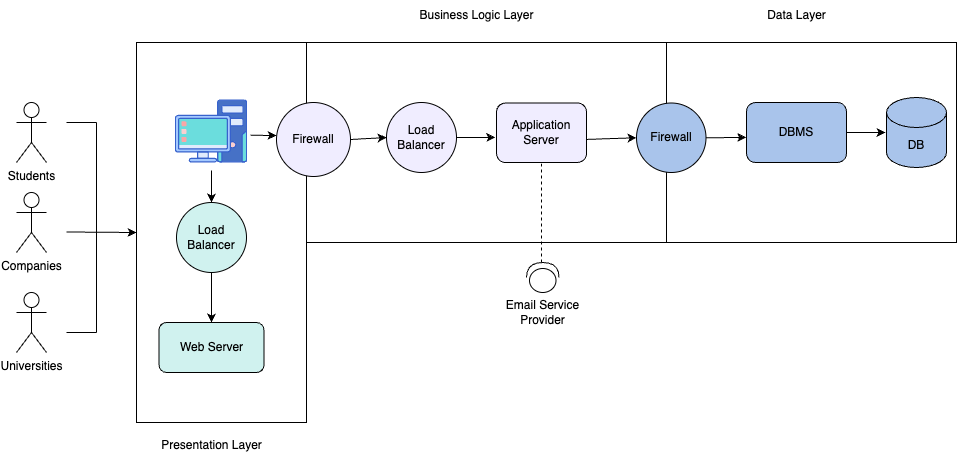
\includegraphics[width=0.8\textwidth]{Images/overview-component.png}
\caption{\label{fig:metamodel4}Presentation Layer, Business Logic Layer and Data Layer}
\end{figure}

\subsection{Component View}
In this section we show the components of the S\&C and their relationships. 

\textbf{Subsystems:}
\begin{enumerate}
    \item \textbf{User Interfaces:}
    \begin{itemize}
        \item \textbf{Student Portal, Company Portal, University Admin Portal:} Interfaces for respective users to interact with the system.
    \end{itemize}

    \item \textbf{Core Systems:}
    \begin{itemize}
        \item \textbf{Recommendation Engine:} Matches students and internships based on data.
        \item \textbf{Feedback and Analytics Module:} Improves recommendations using feedback.
        \item \textbf{Notification Service:} Sends messages/alerts to users.
        \item \textbf{Selection Management System:} Manages interviews and selection processes.
        \item \textbf{Monitoring and Complaints Module:} Tracks internships and manages complaints.
        \item \textbf{Security and Access Control:} Ensures authentication and secure access.
    \end{itemize}

    \item \textbf{Data Storage:}
    \begin{itemize}
        \item \textbf{Database:} Stores CVs, internship details, feedback, and complaints.
    \end{itemize}
\end{enumerate}

\textbf{Connection Types:}
\begin{itemize}
    \item \textbf{\texttt{--( Required Interface:}} Indicates a component requests services (e.g., portals requesting recommendations).
    \item \textbf{\texttt{-(0- Message Interface:}} Represents communication or event-driven messaging (e.g., notifications).
    \item \textbf{\texttt{-0)- Service Interface:}} Represents a request-response model (e.g., selection processes).
    \item \textbf{\texttt{..> Dependency:}} Highlights one component's dependency on another (e.g., feedback improving recommendations).
\end{itemize}

\begin{figure}[H]
\centering
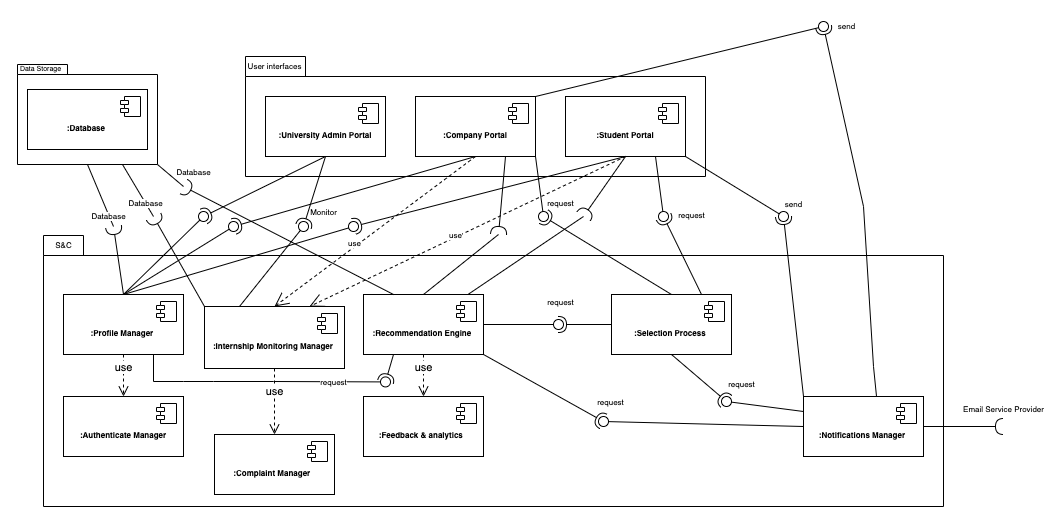
\includegraphics[width=0.8\textwidth]{Images/Component view Diagram.png}
\caption{\label{fig:metamodel4}UML Diagram for Students \& Companies System}
\end{figure}

\subsection{Deployment View}
The S\&C web application is deployed in cloud and uses the benefits that are offered by cloud deployment compared to traditional deployments which will be discussed later.

Client device and access the S\&C web page using any browser of choice. The web pages are loaded from the web server in cloud using HTTP calls. Firewall is used to provide security and allow trusted requests. Elastic load balancer is used to evenly distribute incoming traffic in web servers and application servers. Lastly, the required data are stored in the DB. A standby DB is also added to provide with data connection in case of failure of the main DB. \\ \\

\textbf{Advantages of Cloud - }
\begin{itemize}
\item \textbf{Scalability and Flexibility:} Cloud platforms provide the ability to scale resources up or down quickly based on demand. This is especially useful for businesses with fluctuating needs or growth. Cloud systems automatically scale resources to meet workload changes without manual intervention, optimizing resource utilization.
\item \textbf{Cost Efficiency:} Cloud services offers a pay-per-usage, thus paying only for the resources actually used. Cloud services offer reduced maintenance cost and low infrastructure costs.
\item \textbf{High Availability and Reliability:} Cloud providers usually have data centers in multiple locations, offering built-in redundancy. This ensures high availability and reduces the risk of system outages.
\end{itemize}


\begin{figure}[H]
\centering
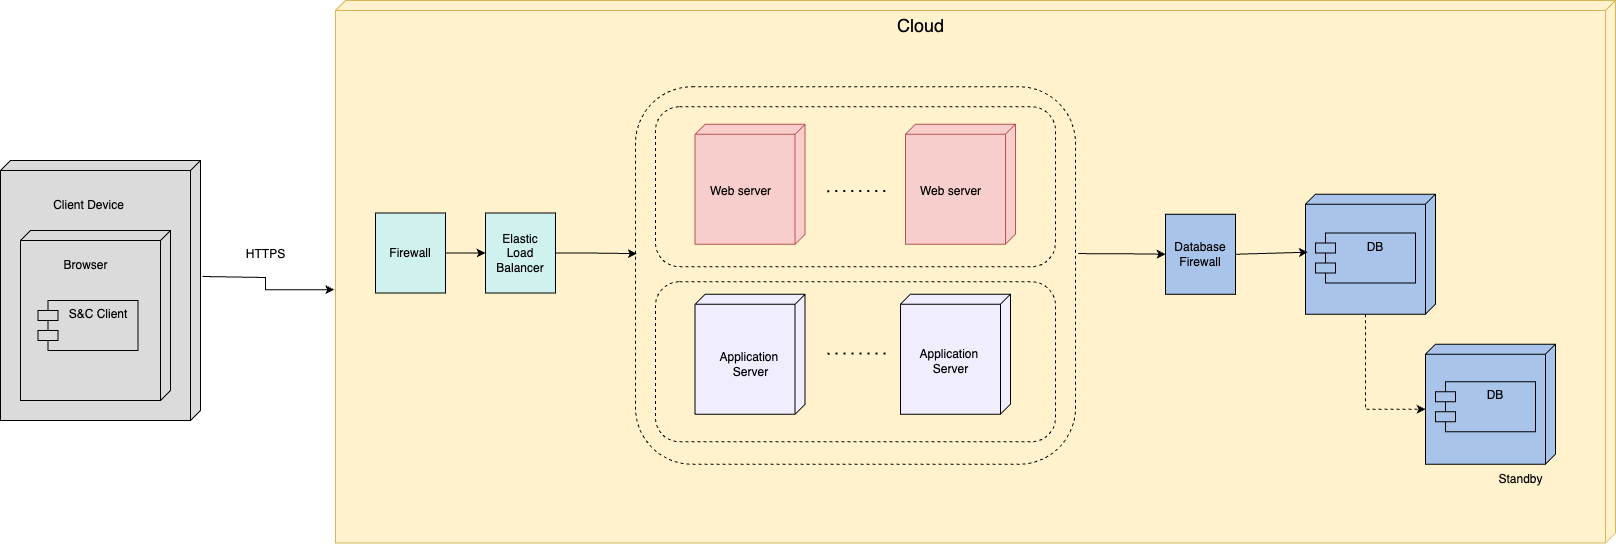
\includegraphics[width=0.8\textwidth]{Images/deployment-view1.png}
\caption{\label{fig:metamodel4}Deployment Diagram}
\end{figure}

\subsection{Runtime View}

\begin{itemize}
    \item \textbf{User Sign Up} \\ \\
    The following diagram is the sequence diagram for the User Sign Up use case depicting all the components engaged for the stated use case. First the User goes to website of S\&C in the browser and tries to Sign Up by giving all the required details. Using API calls the details of the user is sent to the Profile Manager component in the webs server. Profile Manager then sends the data to Entity Manager which connects the database to our server. Then finally data is added to the database. If saving of data is unsuccessful error message is shown to the user else success message is shown.
    \begin{figure}[H]
    \centering
    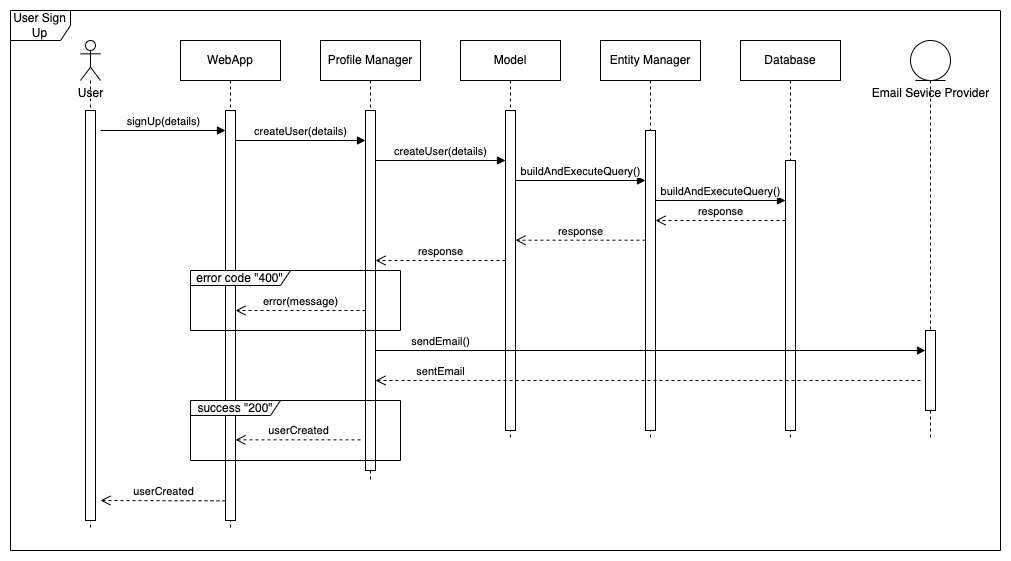
\includegraphics[width=0.8\textwidth]{Images/Sign_Up_Sequence_Diagram.png}
    \caption{\label{fig:metamodel9}[UC1] Sign Up Sequence Diagram.}
    \end{figure}
    \clearpage
    \item \textbf{User Log In} \\ \\
    The following diagram is the runtime sequence diagram for the User Log In use case. When a registered user tries a go on the S\&C WebApp and tries to log in an API request is sent from the client to the Profile Manager component in the web server along with the user entered credentials. These credentials are matched with the stored information in the database. If matched a token is generated by the Authenticate Manager and sent back to the client and the user's profile is visible.
    \begin{figure}[H]
    \centering
    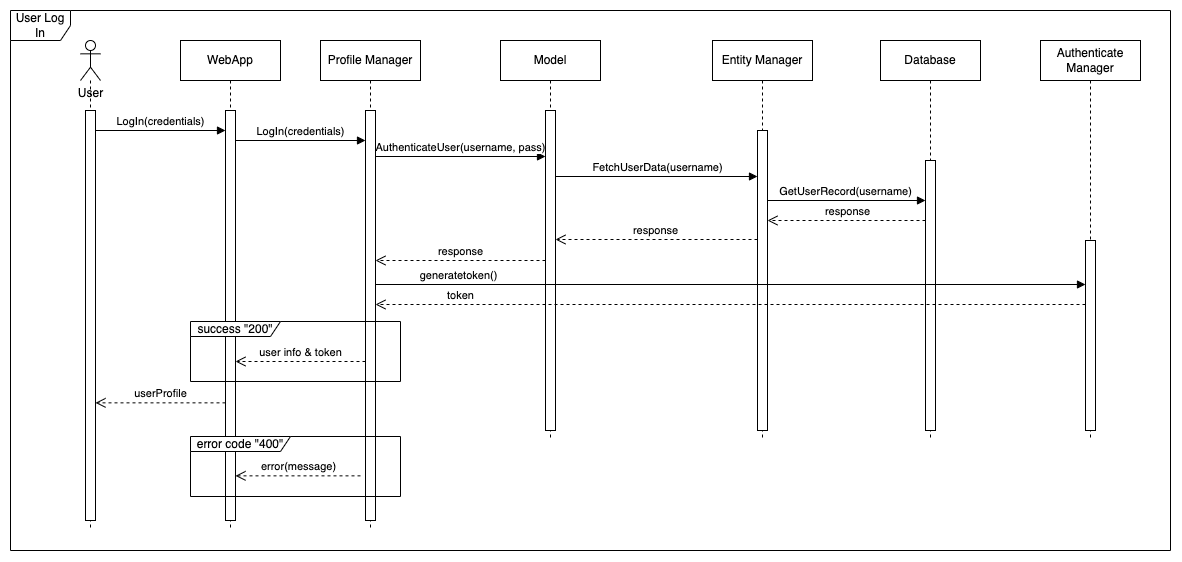
\includegraphics[width=0.8\textwidth]{Images/Log_In_Sequence_Diagram.png}
    \caption{\label{fig:metamodel9}[UC2] Log In Sequence Diagram.}
    \end{figure}
    \item \textbf{Creating CV} \\ \\
    The following diagram is the runtime sequence diagram for the Creating CV use case. A student user can create CV in the S\&C application which is used for applying for internship. For creation of CV the student fills out all the form present in the S\&C browser giving all details like education, skills, experiences etc. Once the user is satisfied the user can click on submit which calls the CreateCV API. The student's CV is ultimately saved in the database.
    \begin{figure}[H]
    \centering
    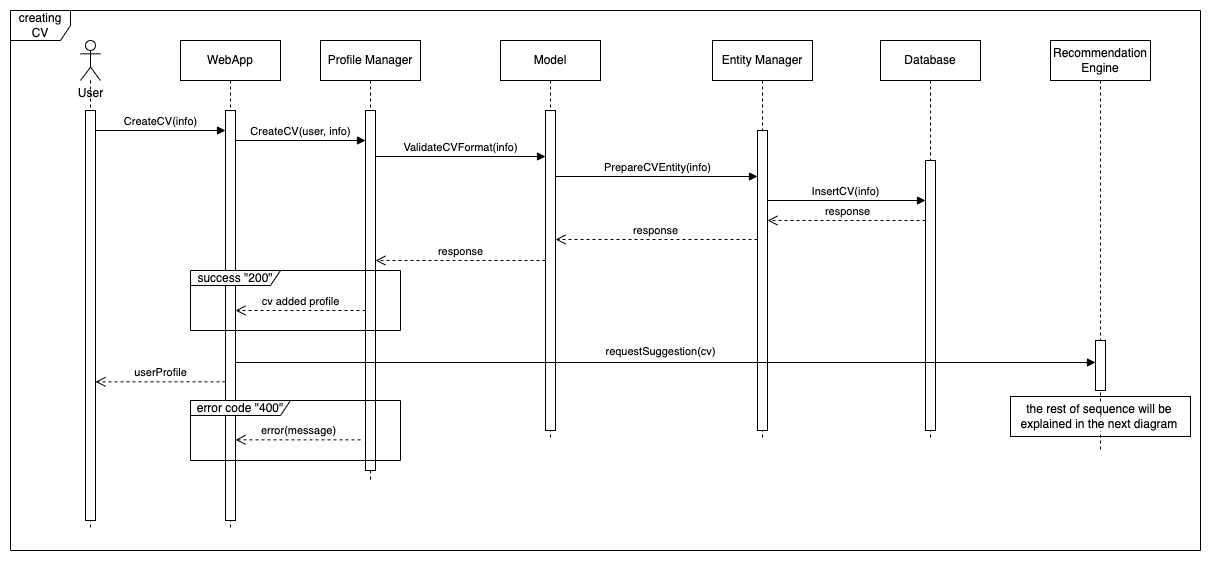
\includegraphics[width=0.8\textwidth]{Images/Creating_CV_Sequence_Diagram.png}
    \caption{\label{fig:metamodel9}[UC3] Creating CV Sequence Diagram.}
    \end{figure}
    \clearpage
    \item \textbf{Get Suggestions on CV} \\ \\
    While writing the CV, student can send requests to the Recommendation Engine in the application to get smart suggestions on the CV content. The Recommendation Engine analyzes the CV and provides tailored suggestions. These suggestions are displayed to the user, who can edit their CV based on the recommendations. Once the user finalizes and saves the edited CV, it is updated and stored in the system's database. The updated CV is reflected on the client-side. The following diagram illustrates the runtime sequence diagram for the Get Suggestions on CV use case.
    \begin{figure}[H]
    \centering
    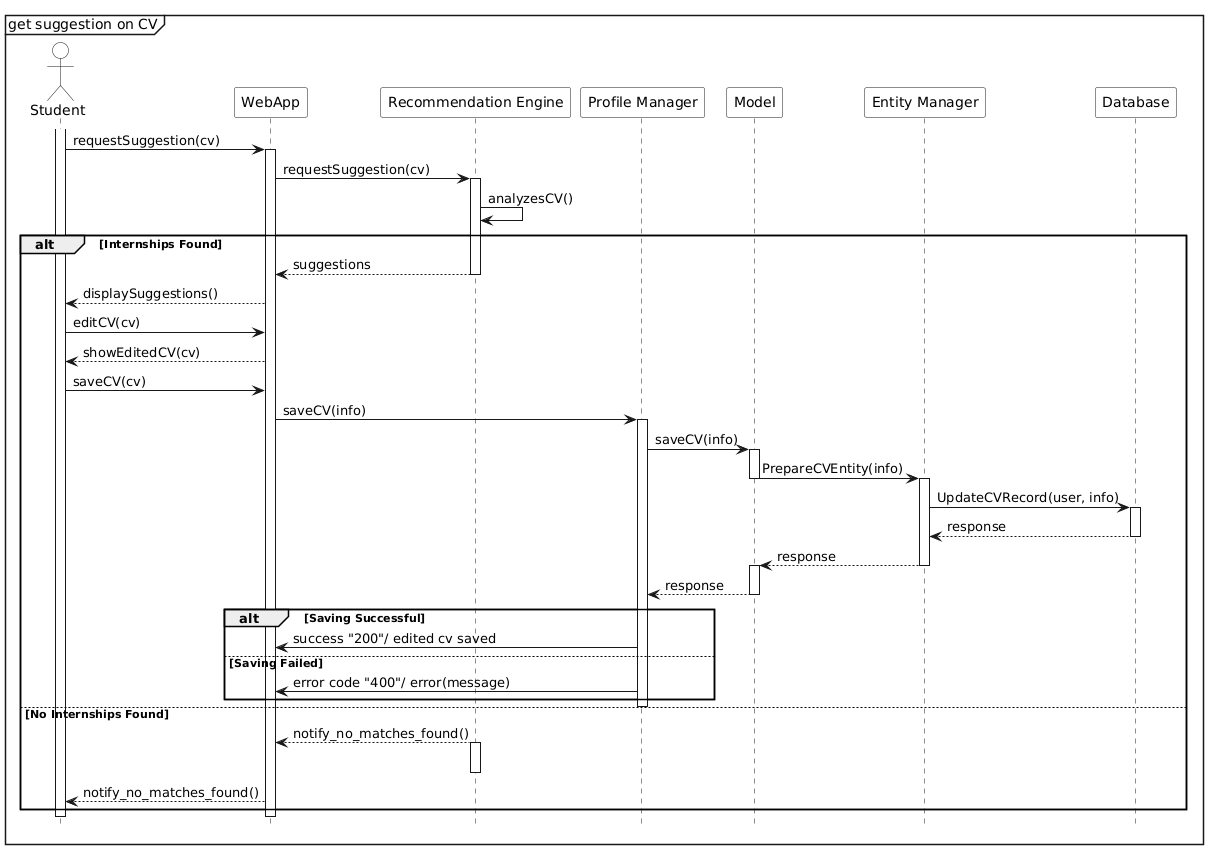
\includegraphics[width=0.8\textwidth]{Images/CV_Suggestion_Sequence_Diagram.png}
    \caption{\label{fig:metamodel9}[UC4] Get suggestion on CV Sequence Diagram.}
    \end{figure}
    \clearpage
    \item \textbf{Post Internship Advertisement} \\ \\
    After logging-in in the S\&C website a company recruiter can post internship advertisement. To post the user fills out all the necessary details related to the internship position like job description, skills required, compensation in the website and then clicks on "Post" button and all the details related to the job is then saved in the Database. The user is then returned to their profile where they can see the posted internship. The following diagram is the runtime sequence diagram for the Post Internship Advertisement use case.
    \begin{figure}[H]
    \centering
    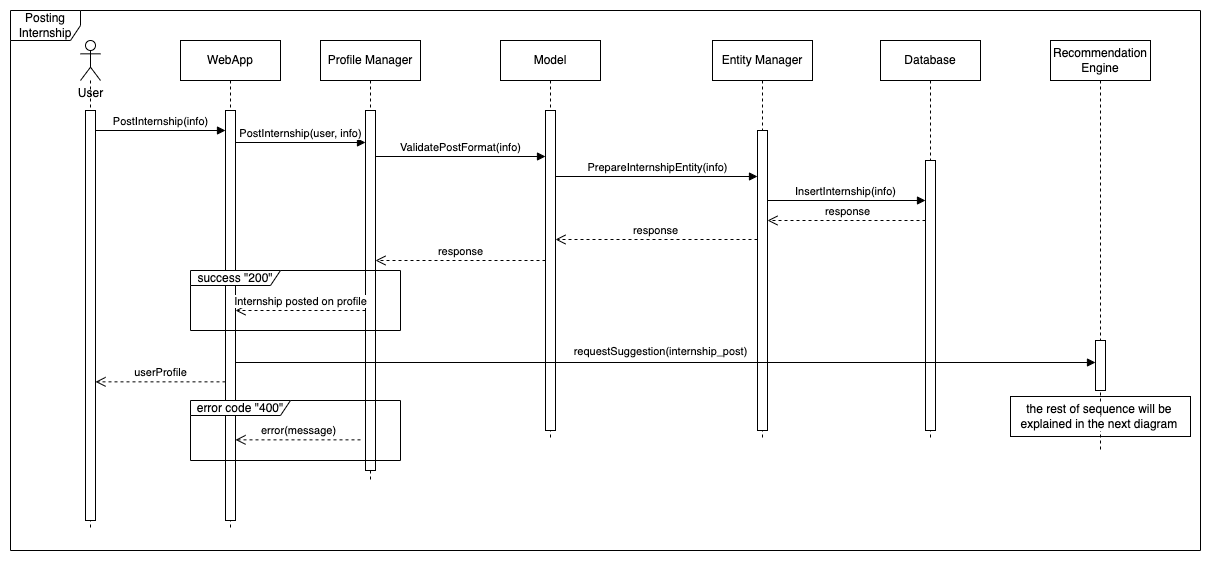
\includegraphics[width=0.8\textwidth]{Images/Posting_Internship_Sequence_Diagram.png}
    \caption{\label{fig:metamodel9}[UC5] Post Internship Sequence Diagram.}
    \end{figure}
    \clearpage
    \item \textbf{Get Suggestions on Ad} \\ \\
    During the writing of an internship advertisement, companies can request suggestions from the S\&C system to enhance the post. The content of the job post is sent to the Recommendation Engine, which analyzes the content and provides suggestions to improve the advertisement. These suggestions are displayed to the company user, who can either edit and finalize the ad or reject the suggestions. Once the edited advertisement is saved, it is updated in the system and reflected in the database. The following diagram illustrates the runtime sequence diagram for the Get Suggestions on Ad use case.
    \begin{figure}[H]
    \centering
    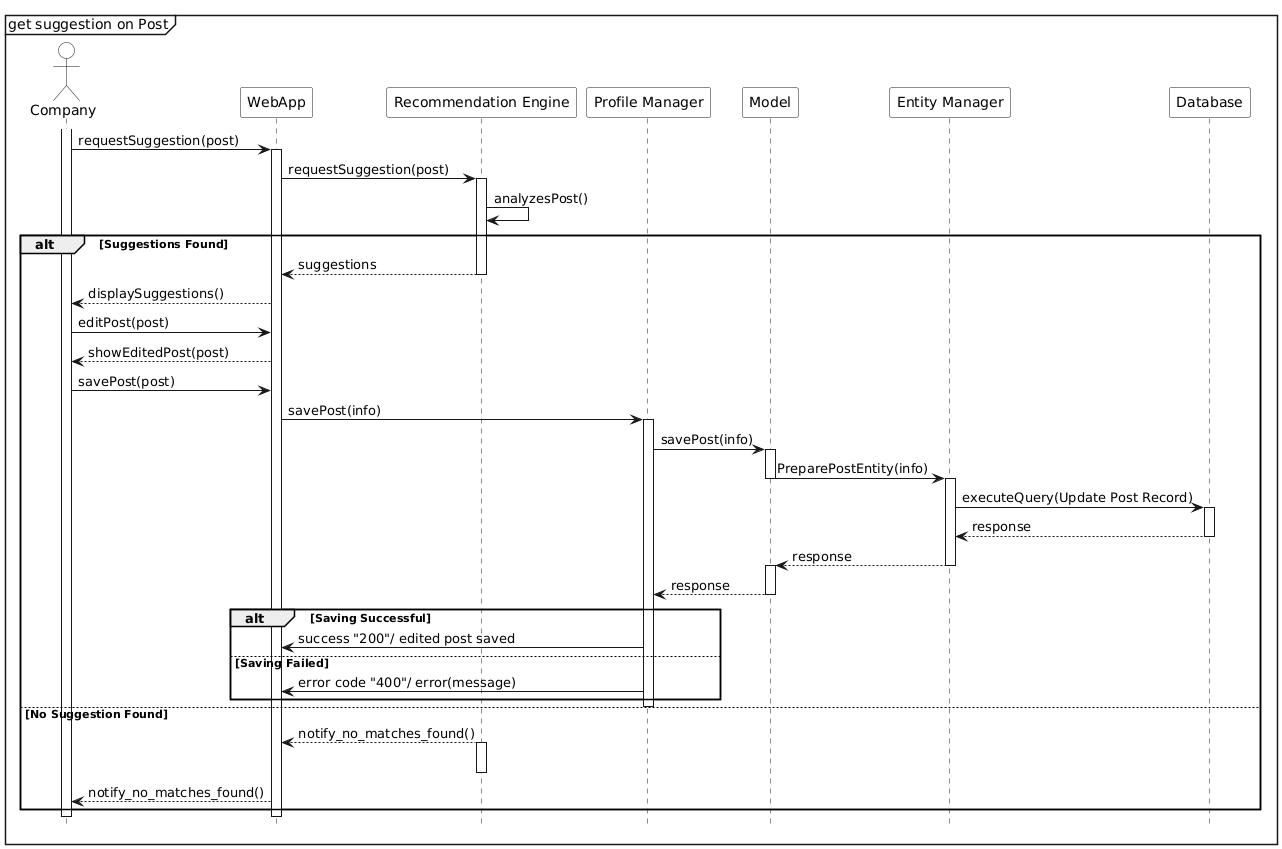
\includegraphics[width=0.8\textwidth]{Images/Internship_Suggestion_Sequence_Diagram.png}
    \caption{\label{fig:metamodel9}[UC6] Get suggestion on Internship Post Advertisement Sequence Diagram.}
    \end{figure}
    \item \textbf{Define a Questionnaire} \\ \\
    After posting an internship post the company personnel can create a Questionnaire to be sent to the students who are shortlisted for the next step. The company personnel can define the questionnaire for a particular internship offer by fetching details of the internship from the server. Once satisfied the user saves then questionnaire in the database for later use. The following diagram is the runtime sequence diagram for the Define a Questionnaire use case.
    \begin{figure}[H]
    \centering
    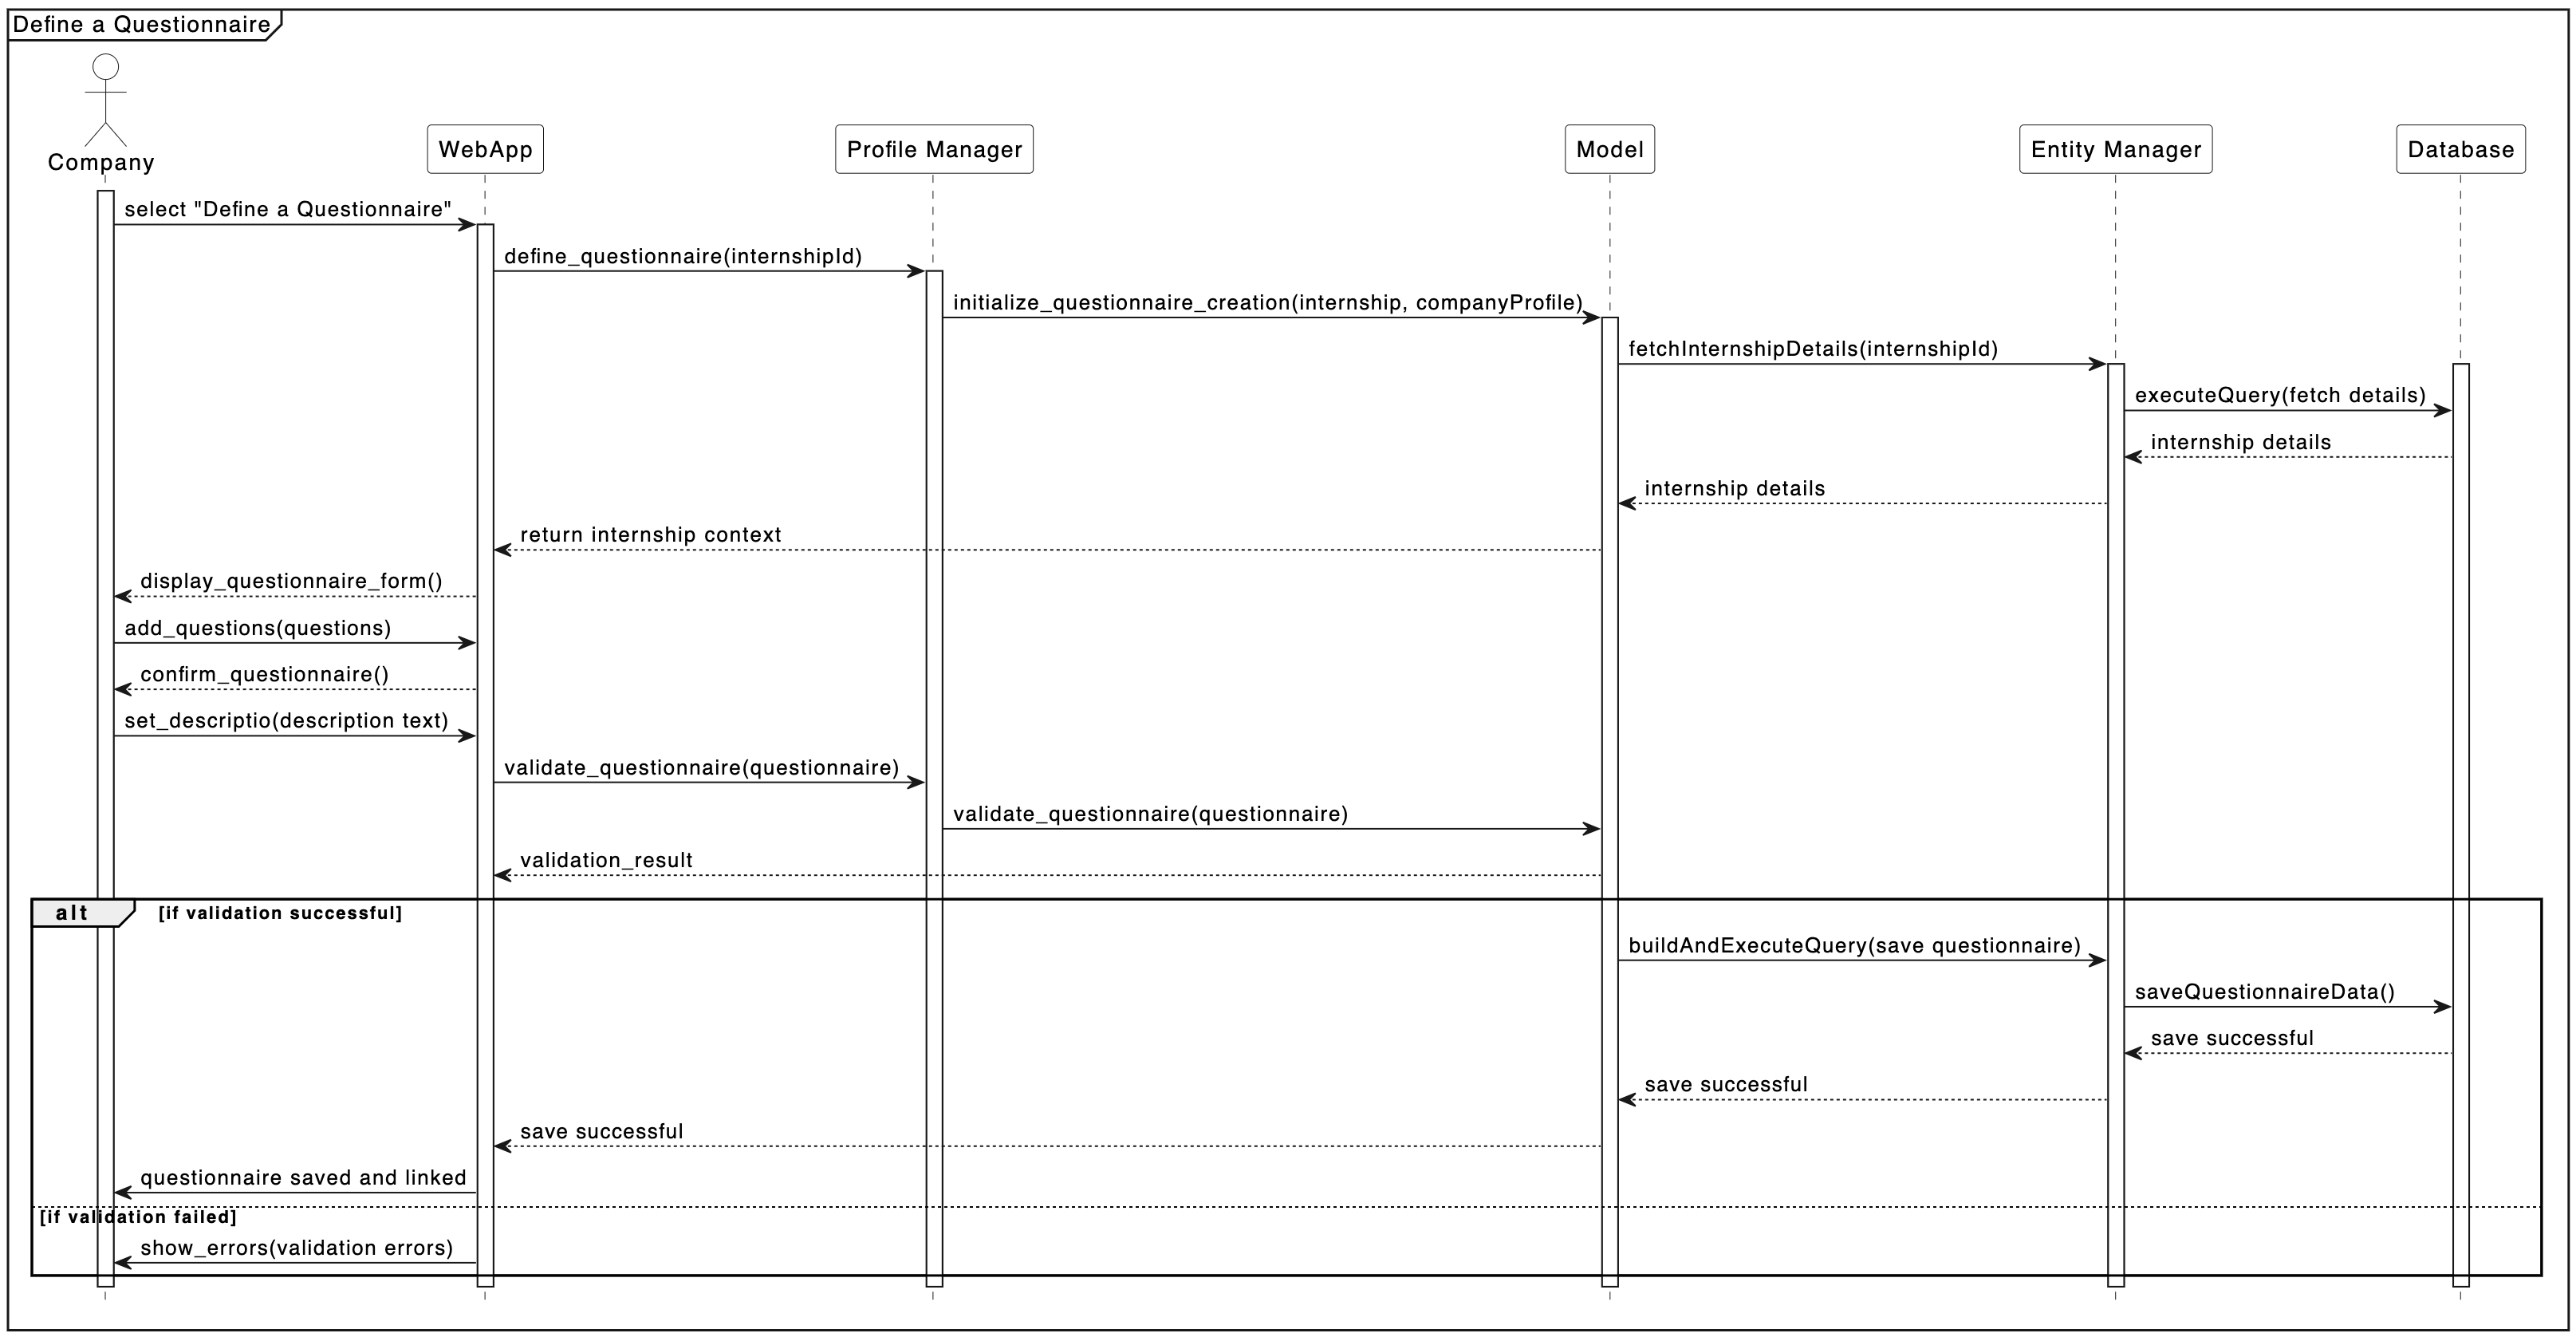
\includegraphics[width=0.8\textwidth]{Images/Define_Questionnaire_Sequnce_Diagram.png}
    \caption{\label{fig:metamodel9}[UC7] Define a Questionnaire for the Internship Post Sequence Diagram.}
    \end{figure}
    \item \textbf{Search Internship} \\ \\
    Students can search for internship by typing required keywords like job roles, position, location in the search internship tab of the S\&C website. ElasticSearch will be used for filtering and available internships are sent to the student. The student can then open each internship and view it's details. The following diagram is the runtime sequence diagram for the Search Internship use case.
    \begin{figure}[H]
    \centering
    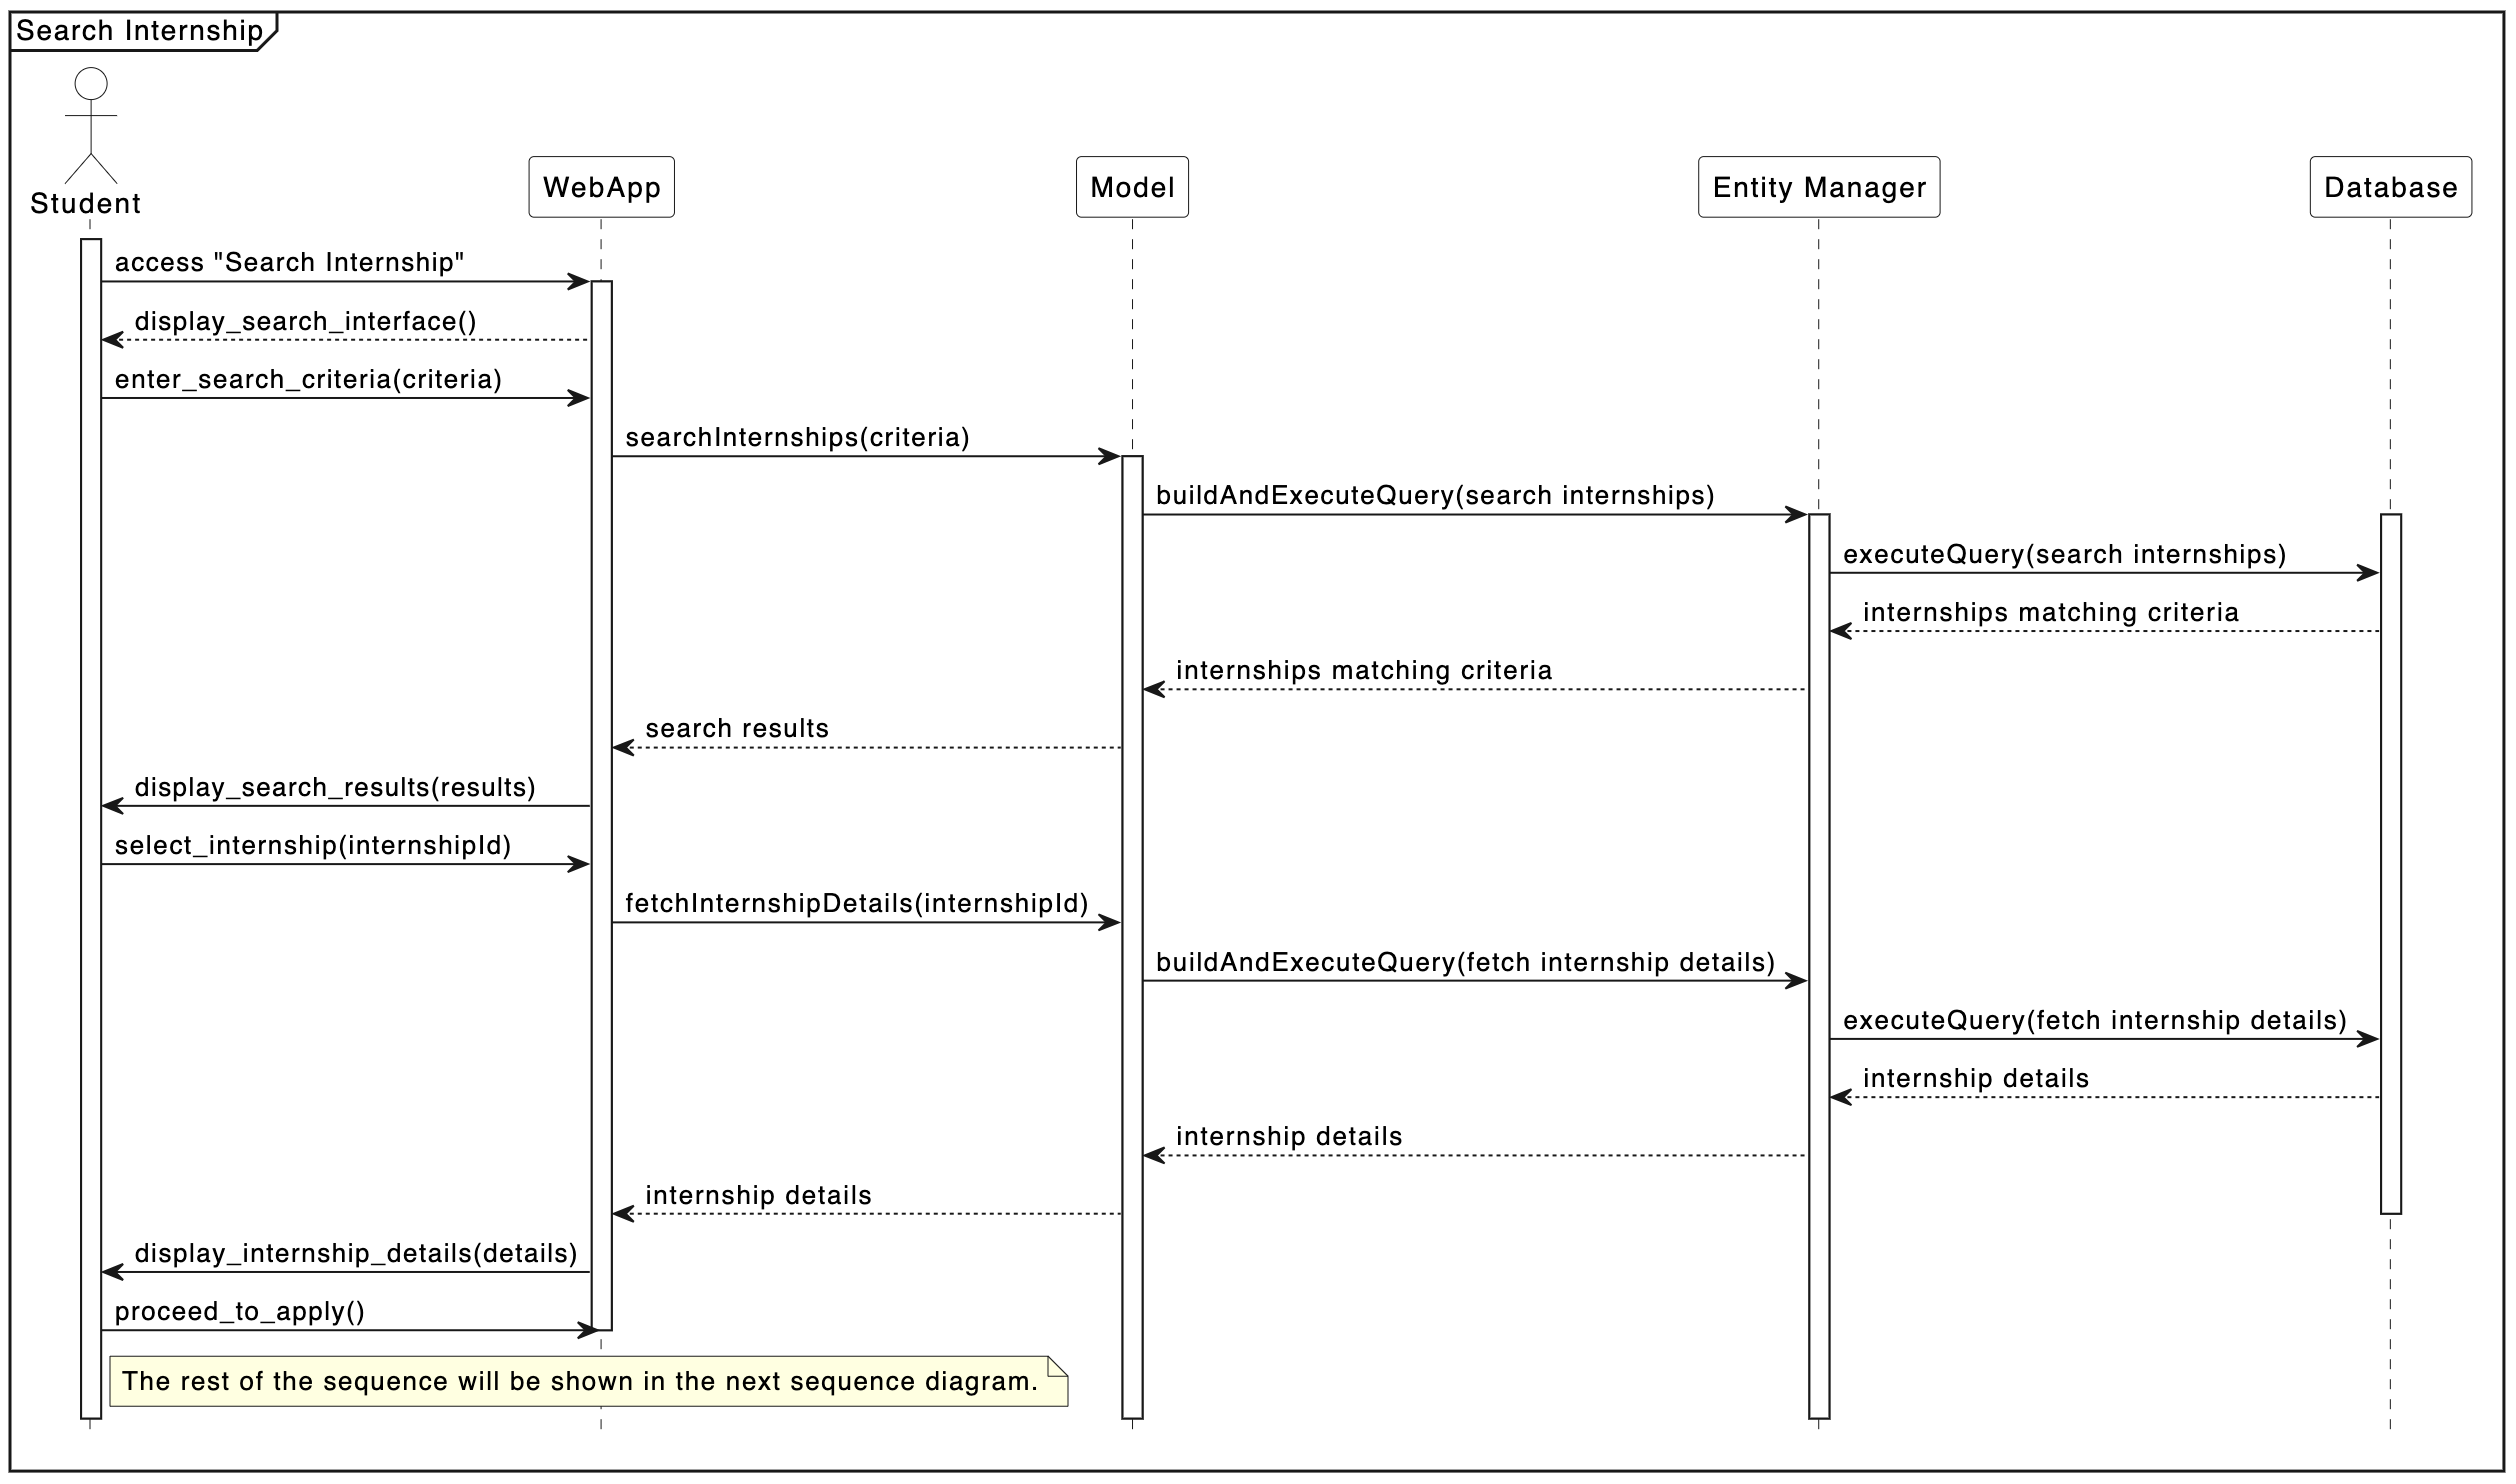
\includegraphics[width=0.8\textwidth]{Images/Search_Internship_Sequence_Diagram.png}
    \caption{\label{fig:metamodel9}[UC8] Search Internship Sequence Diagram.}
    \end{figure}
    \item \textbf{Apply Internship} \\ \\
    A student can apply to any desired internship post by clicking on the "Apply" button. Student will be prompted to select application materials like CV, cover letter. Once selected the students application for that internship will be saved in the database. Once applied is submitted Notification Manager will send notification to the company. The following diagram is the runtime sequence diagram for the Apply Internship use case.
    \begin{figure}[H]
    \centering
    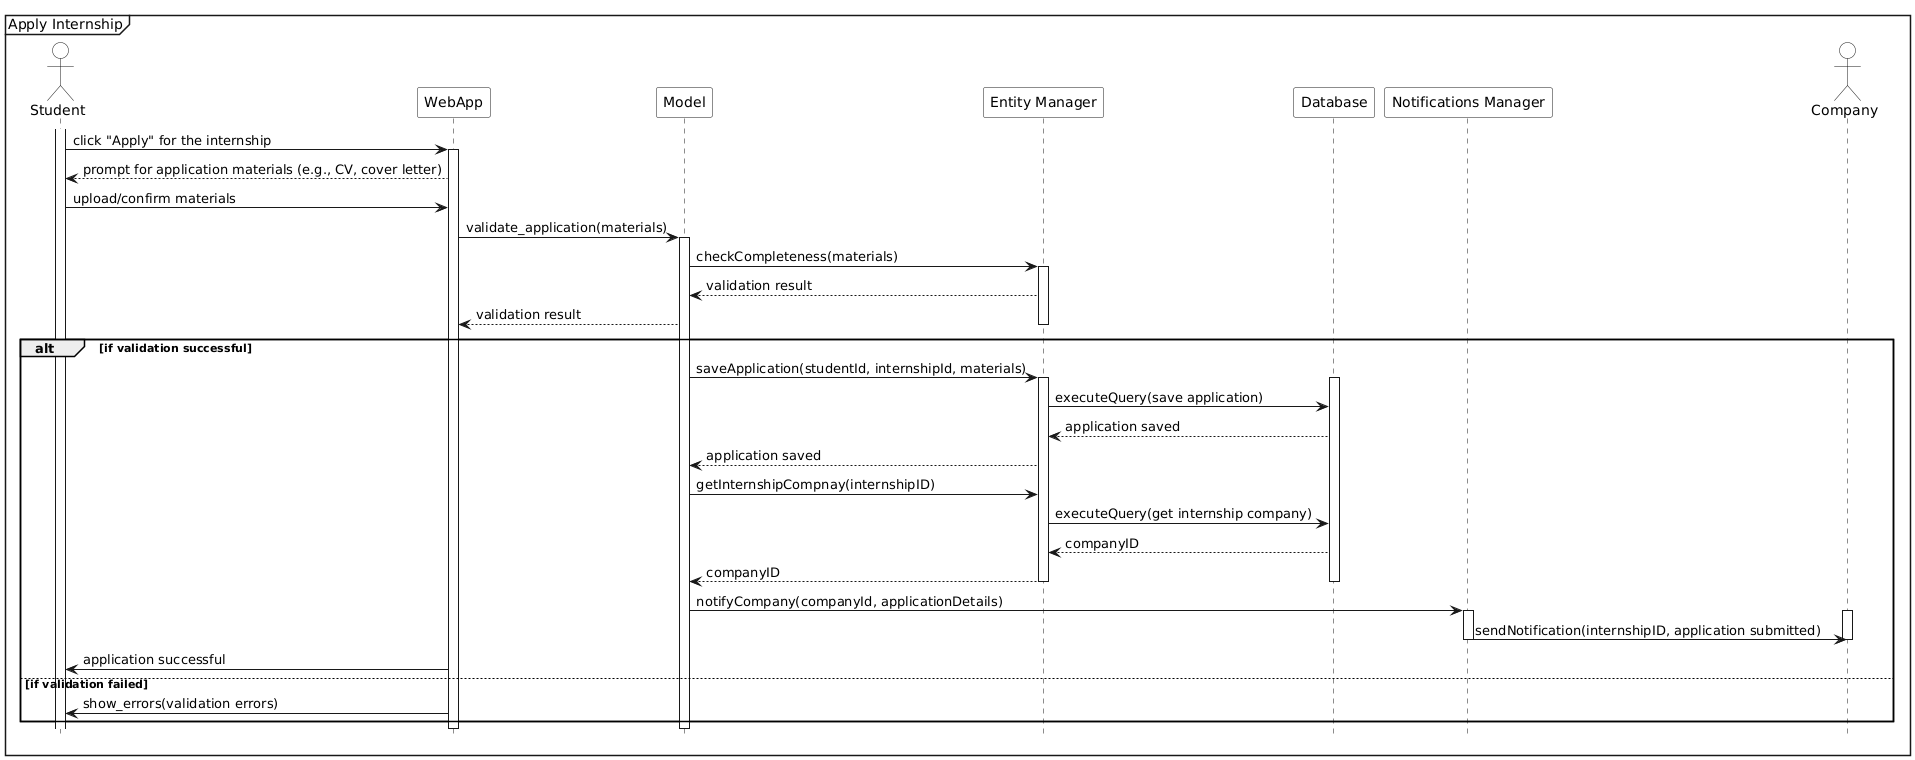
\includegraphics[width=0.8\textwidth]{Images/Apply_Internship_Sequence_Diagram.png}
    \caption{\label{fig:metamodel9}[UC9] Apply Internship Sequence Diagram.}
    \end{figure}
    \item \textbf{Accept/Reject Application} \\ \\
    A company recruiter can view the applications of students who have applied for their internship post. Company recruiter can fetch the the list of all applicants. Then user then clicks on "Accept" or "Reject" for all applications for the next step. The students are notified of the same. The application status of each application is then updated accordingly in the database. The following diagram is the runtime sequence diagram for the Accept/Reject Application use case.
    \begin{figure}[H]
    \centering
    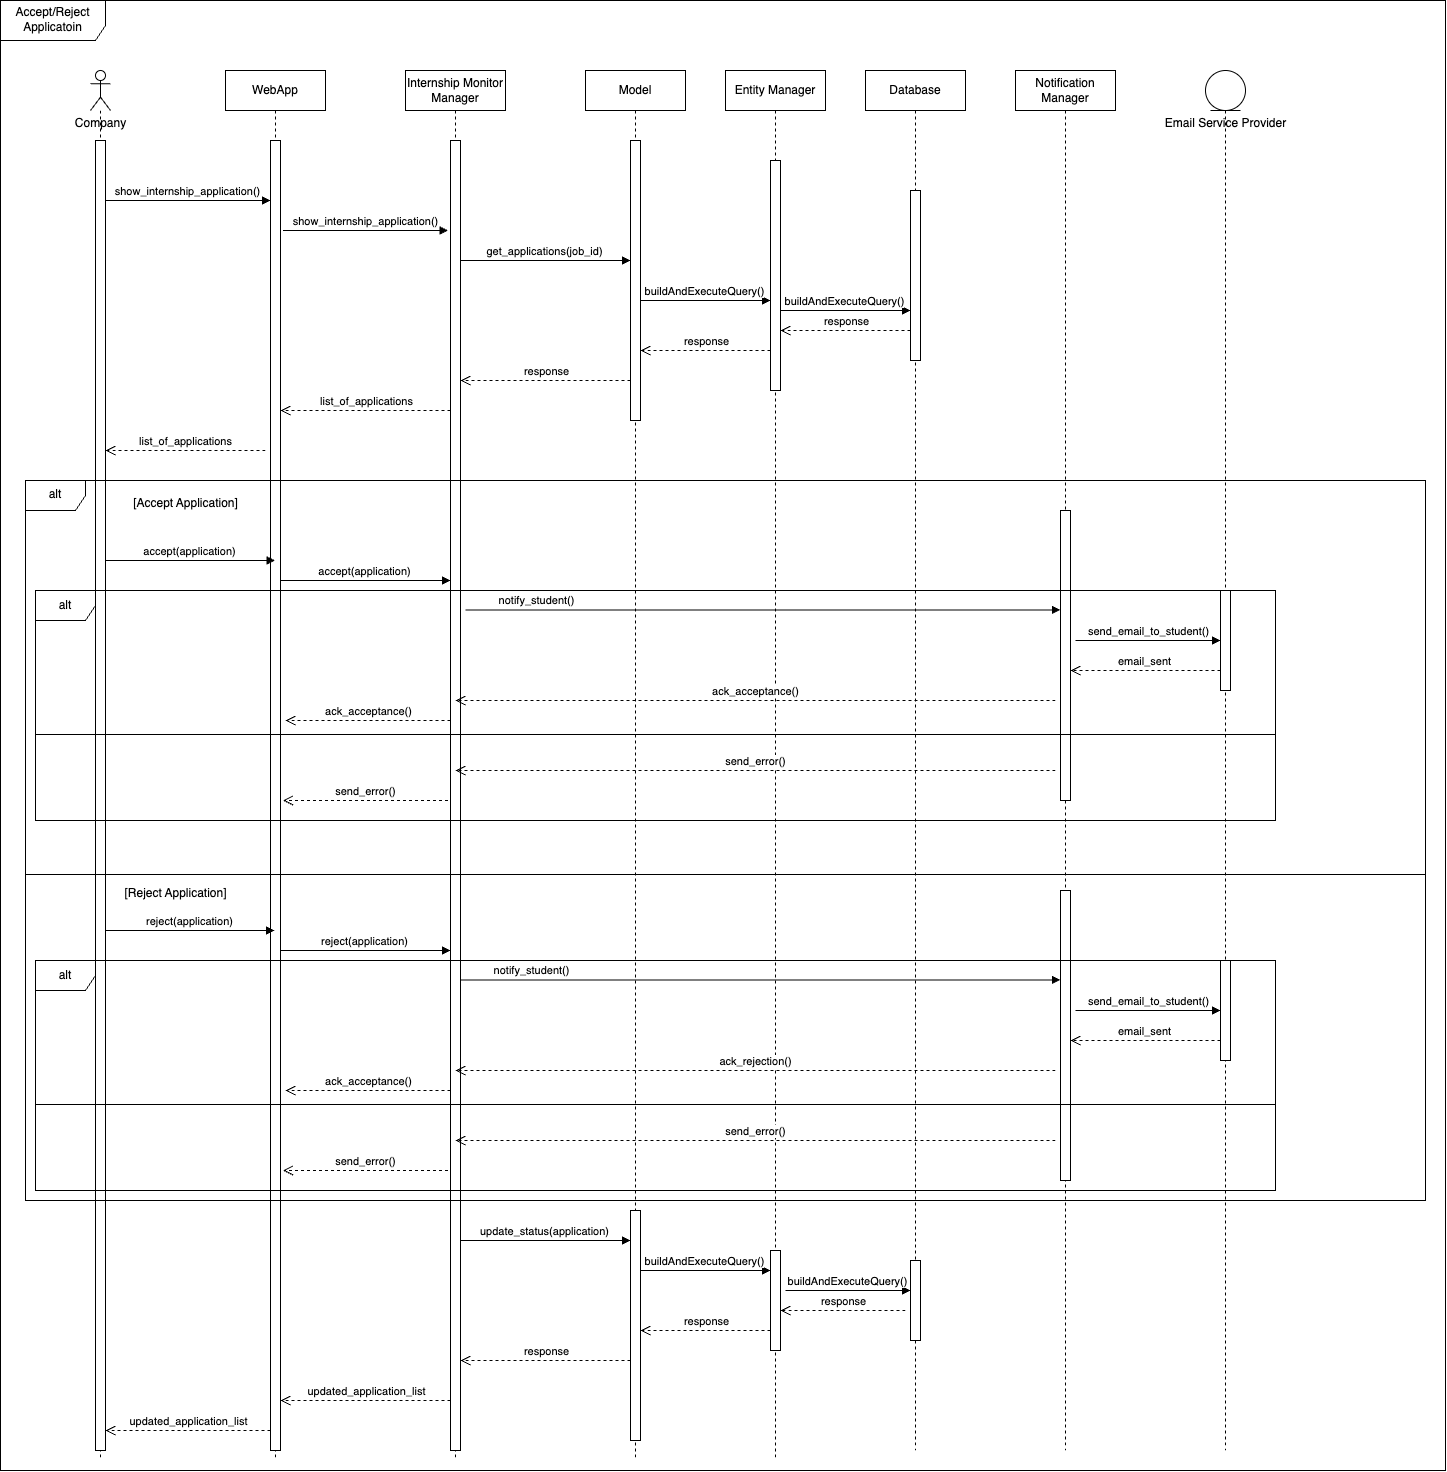
\includegraphics[width=0.8\textwidth]{Images/Accept_reject_sequence_diagram.png}
    \caption{\label{fig:metamodel9}[UC10] Accept/Reject Application Sequence Diagram}
    \end{figure}
    \item \textbf{Match Students and Internships} \\ \\
    In S\&C platform matchmaking system is there to notify students of available internship and notify companies and eligible students with required characteristics for an open internship are available. Recommendation Engine analyses CVs of students and descriptions of internships and for each student creates list of suitable companies and for each company creates list of suitable candidates and notifies each parties using email. This recommendation process is carried out at a periodic interval (for e.g. every 24 hours). The following diagram is the runtime sequence diagram for the Match Student and Internship Sequence Diagram use case.
    \begin{figure}[H]
    \centering
    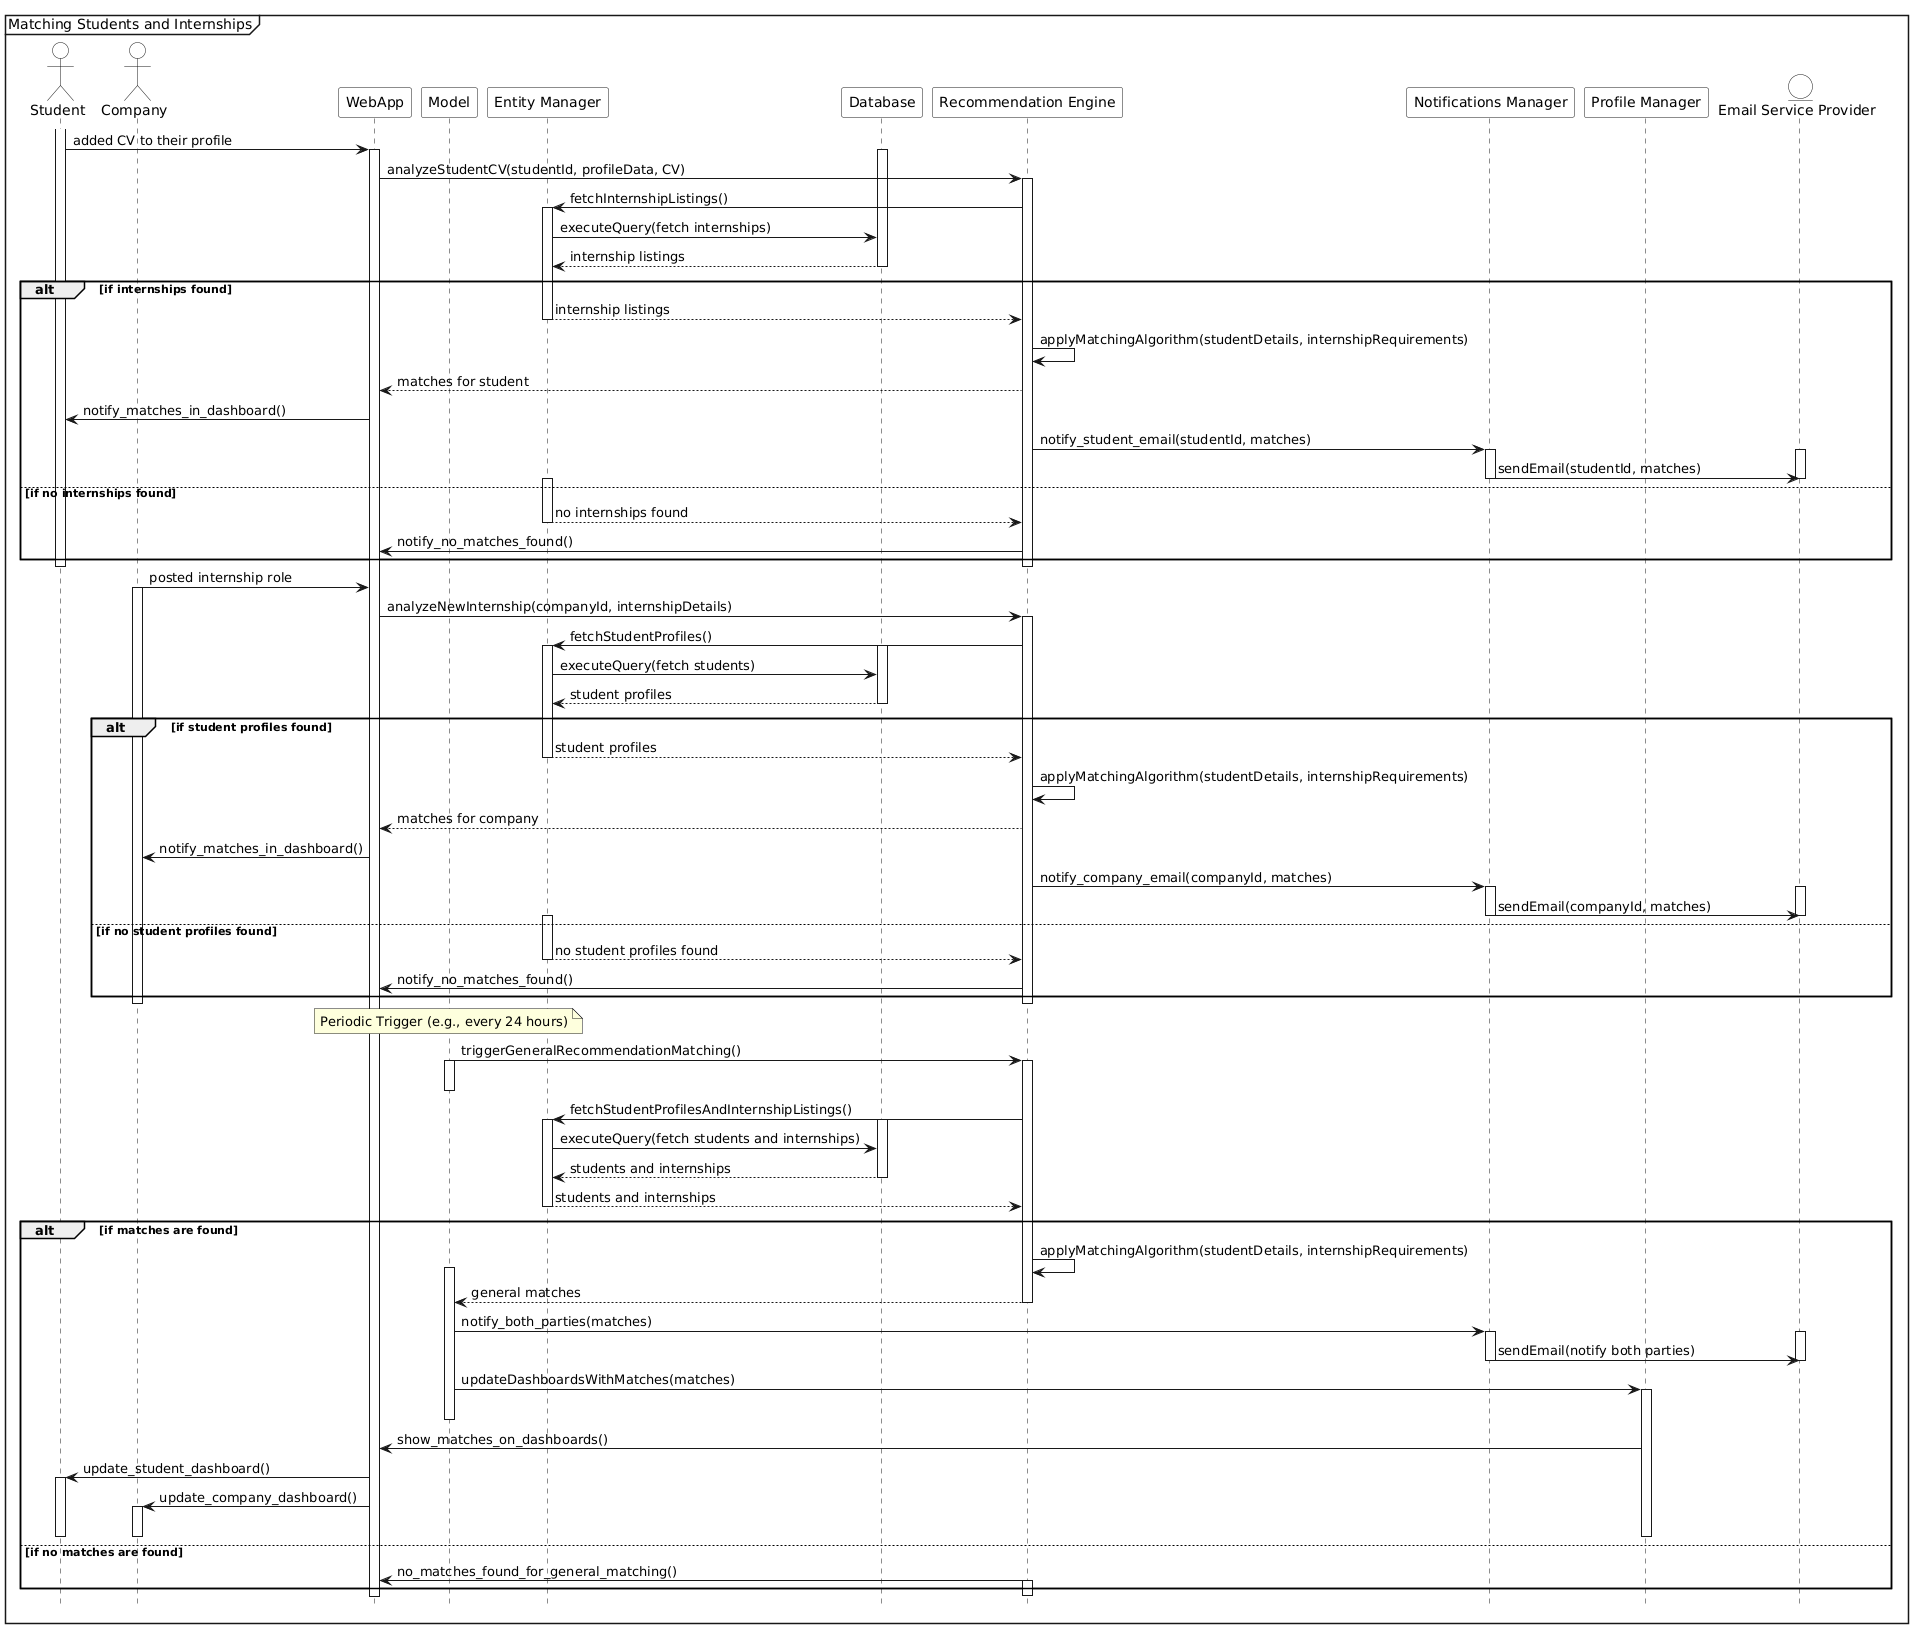
\includegraphics[width=0.8\textwidth]{Images/Match_Student_Internship_Sequence_diagram.png}
    \caption{\label{fig:metamodel9}[UC11] Match Student and Internship Sequence Diagram}
    
    \end{figure}
    \item \textbf{Selection Process} \\ \\
    Once a company accepts an application or a match-making recommendation is accepted by both the company and student the selection process starts. A communication channel is opened between the company and the student both the parties are notified. The previously defined questionnaire is forwarded to the student to be answered. The Student then fills up the questionnaire and submits it which is then can be read by the company. The company can then either select the student for the interview or reject them. In the both the cases the students will be notified and the selected student will be added to the interview shortlist. The following diagram is the runtime sequence diagram for the Selection Process Sequence Diagram use case.
    \begin{figure}[H]
    \centering
    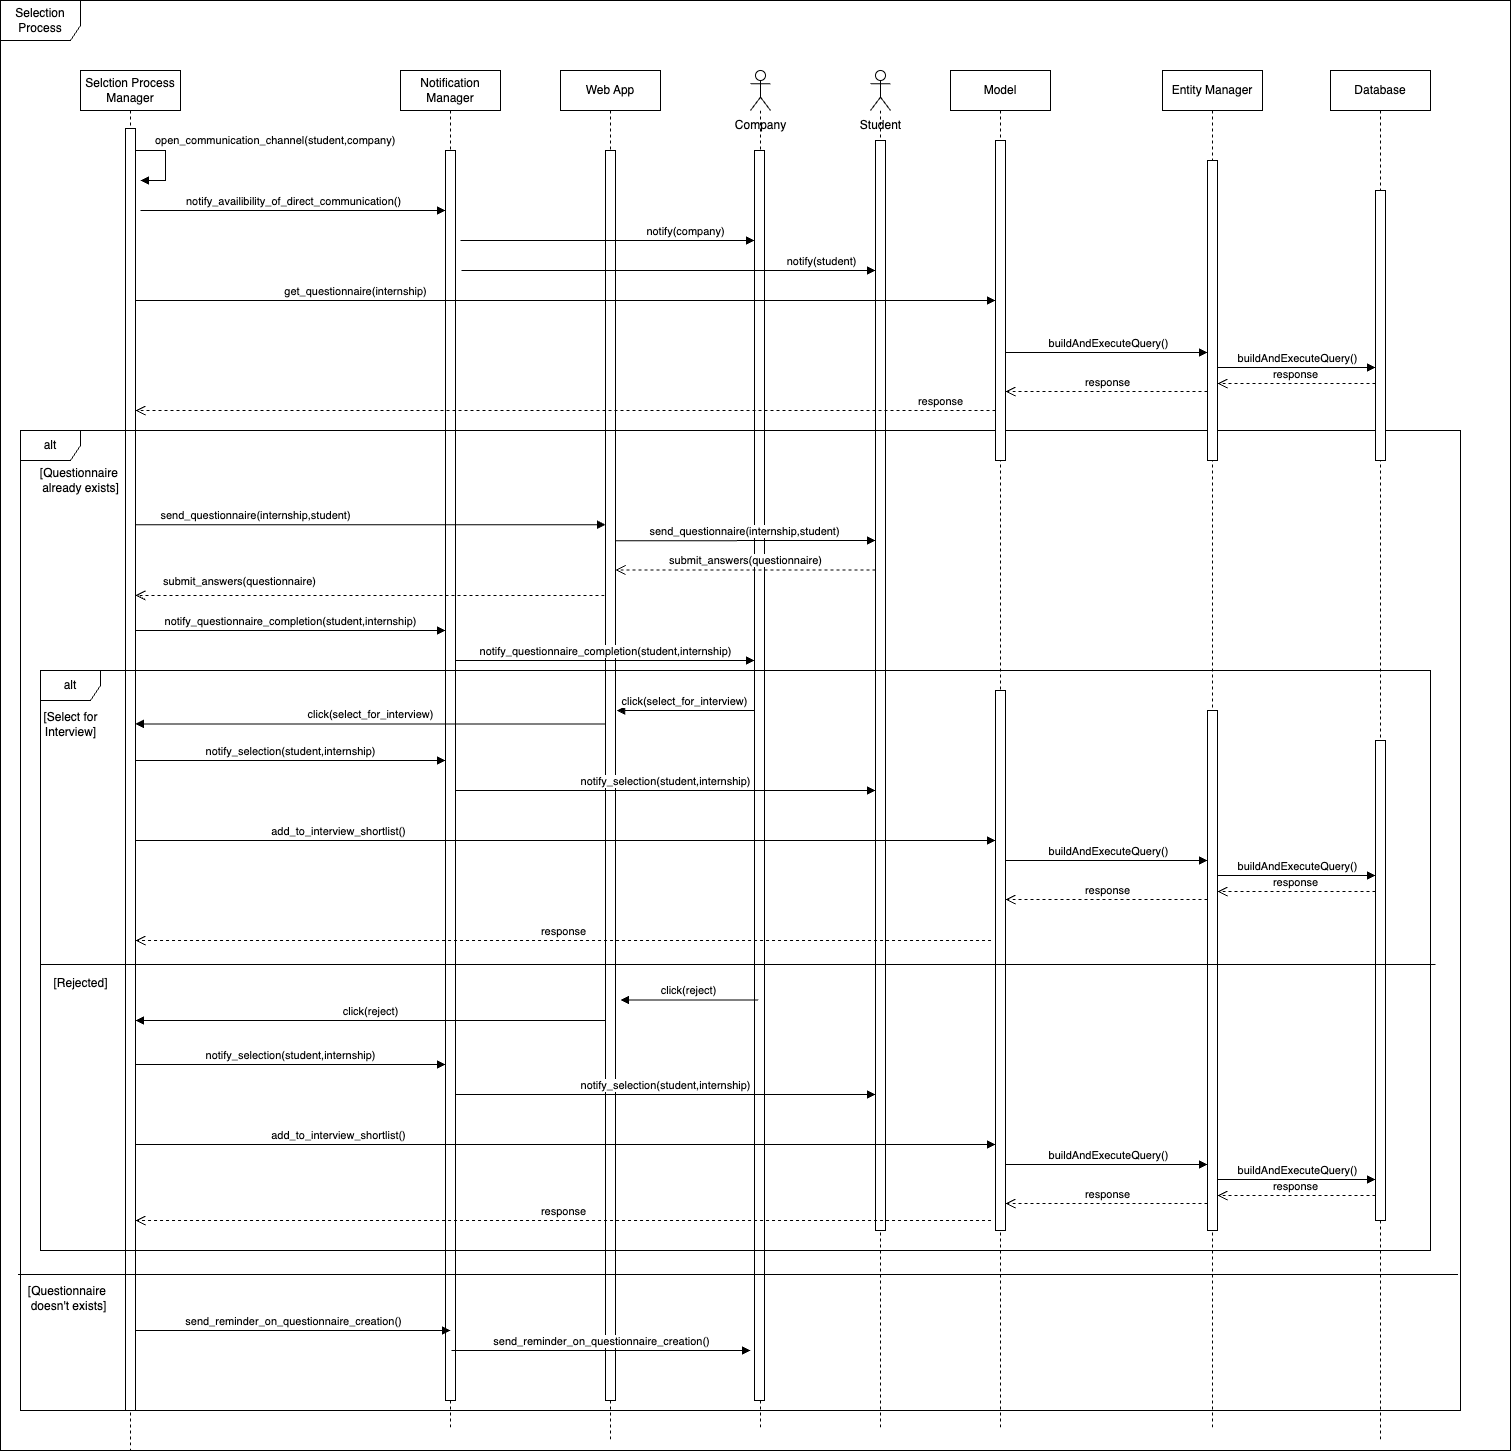
\includegraphics[width=0.8\textwidth]{Images/select_process_seq_diag.png}
    \caption{\label{fig:metamodel9}[UC12] Selection Process Sequence Diagram}
    \end{figure}
    
    \item \textbf{Set Up Interview (S\&C Platform Manage Interview Process)} \\ \\
    Once company selects a student for interview the Selection Process Manager will request both student and company to select range of available dates in the calender. Once dates are selected an interview date will be selected and interview details along with dates and location or interview link will be sent to both the student and company using Notification Manager and the data will be saved in the database. The following diagram is the runtime sequence diagram for the Set Up Interview (S\&C Platform Manage Interview Process) Sequence Diagram use case.
    \begin{figure}[H]
    \centering
    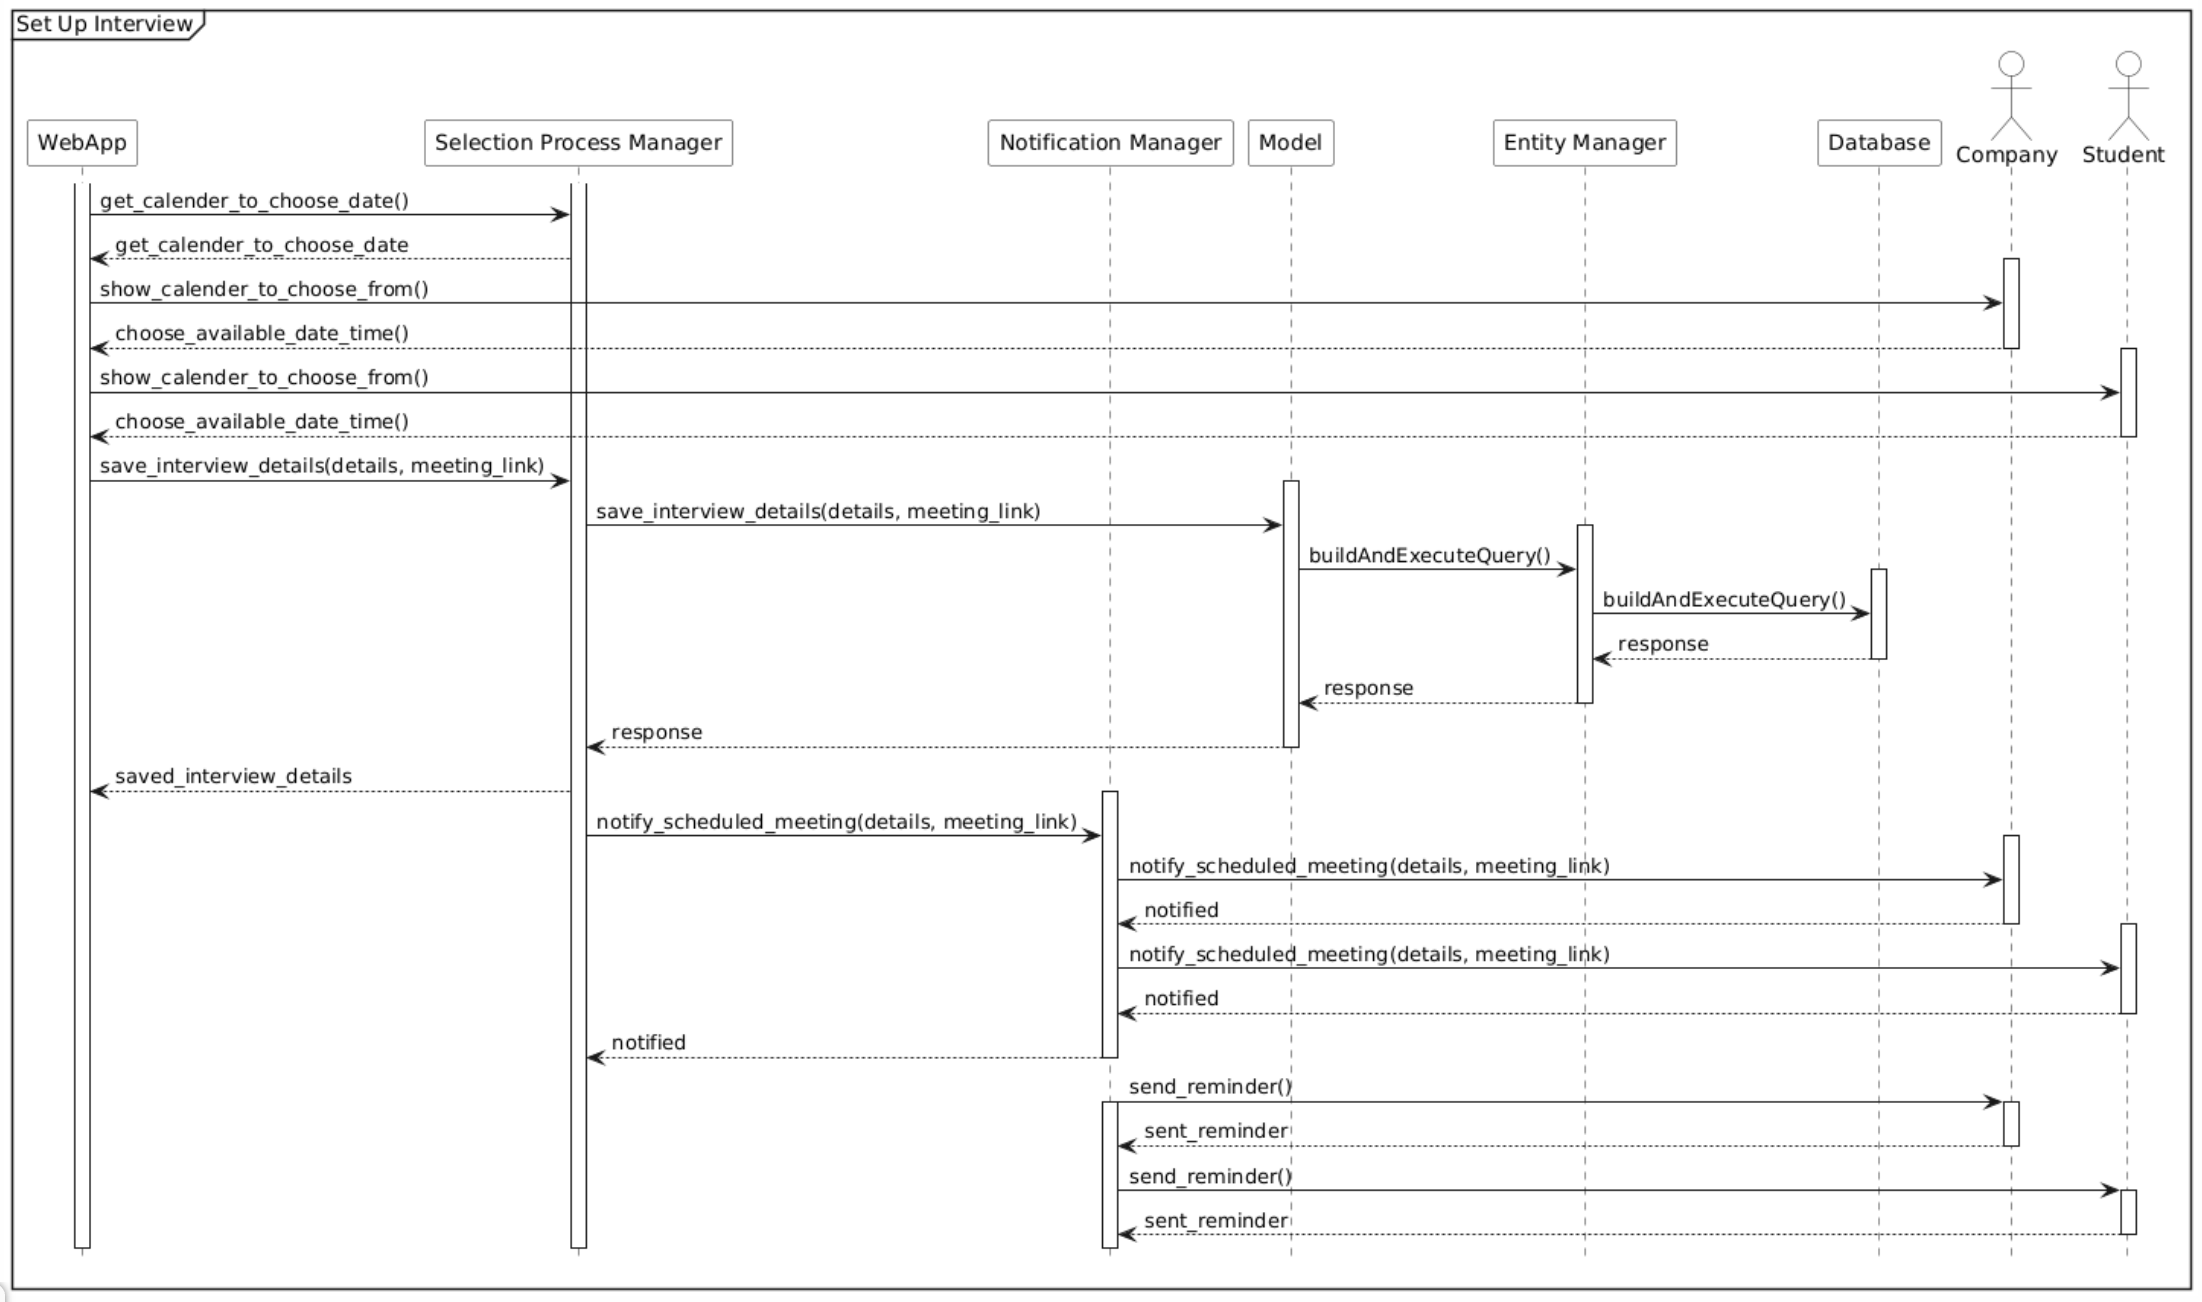
\includegraphics[width=0.8\textwidth]{Images/set_up_interview_sequence1.png}
    \caption{\label{fig:metamodel9}[UC13] Set Up Interview Sequence Diagram}
    \end{figure}
    \item \textbf{Finalize Decision (company finalize the decision for selection process)} \\ \\
    Company can see the lift of the interview students and from there hire or reject a student for that post. If the company decides to hire a student notification is sent to that student. If the company rejects then notification is sent to that student. The decisions are then updated in the databases. If no students have been interviewed yet it is reflected in the website. The following diagram is the runtime sequence diagram for the Finalize Decision Sequence Diagram use case.
    \begin{figure}[H]
    \centering
    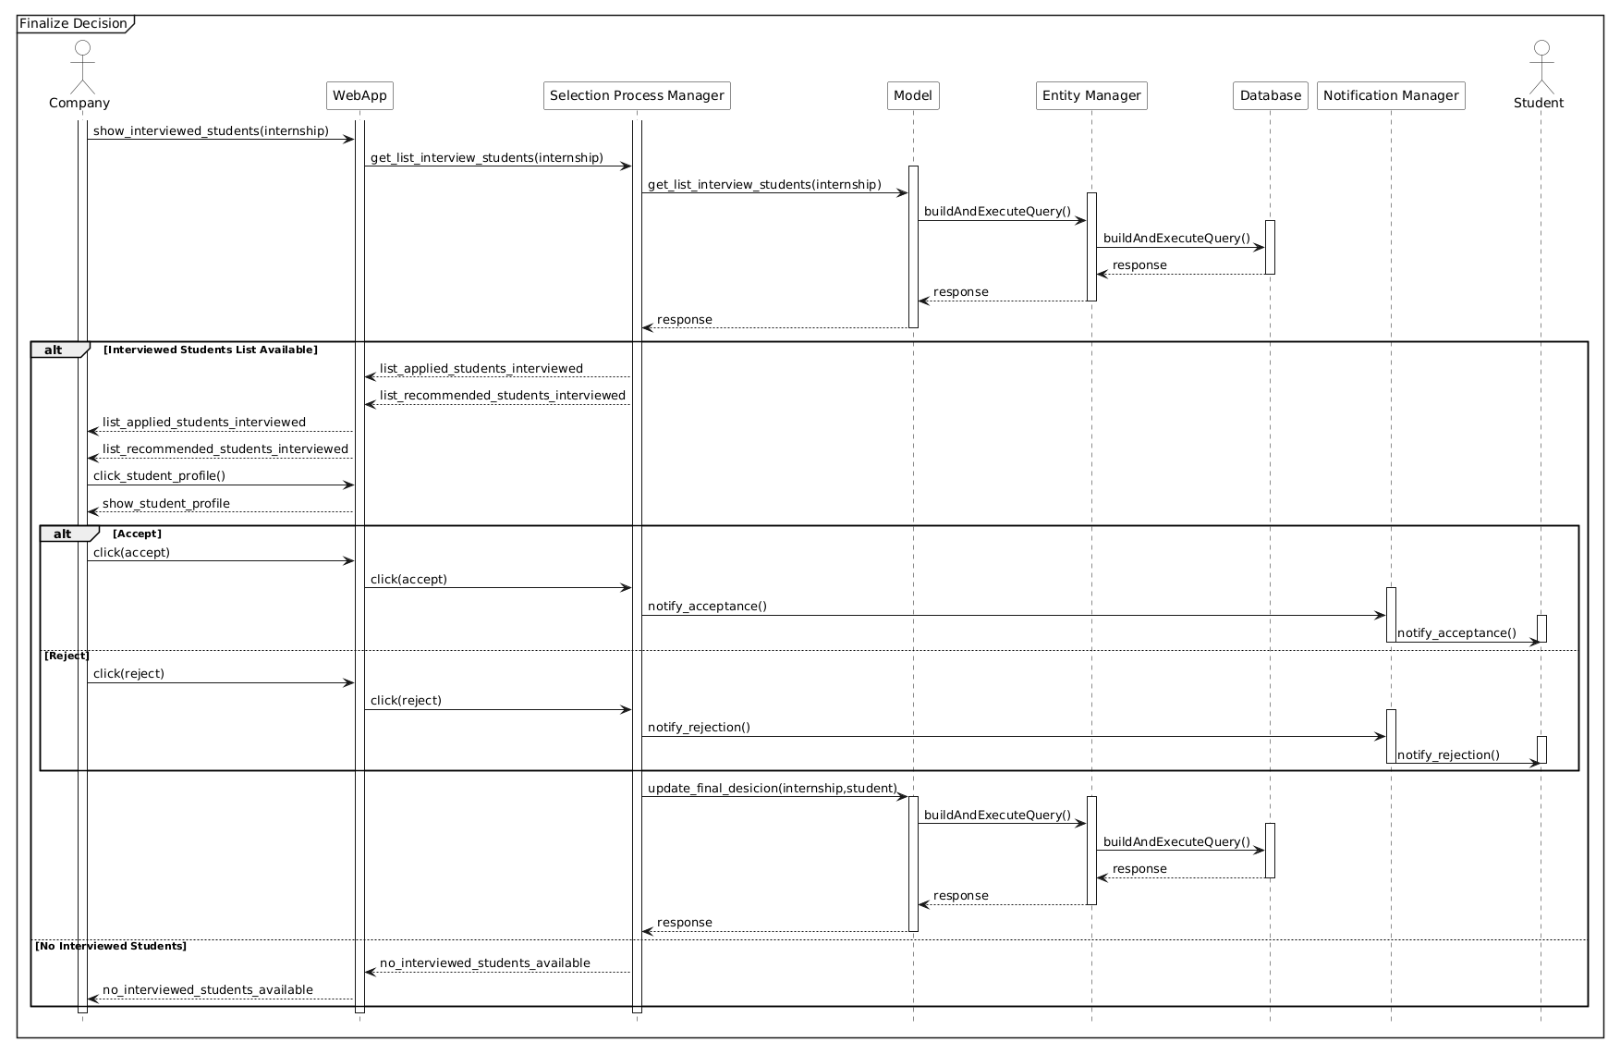
\includegraphics[width=0.8\textwidth]{Images/Finalize-decision-sequence-diagram.png}
    \caption{\label{fig:metamodel9}[UC14] Set Up Interview Sequence Diagram}
    \end{figure}
    \clearpage
    \item \textbf{Collect Feedback} \\ \\
    After completion of the interview or while using of the application the students and companies are requested by the Feedback and Analytics manager to give feedback on the website and it's applications. The feedback given by the users are send saved in the database. The feedback is then used by the developers of the system to improve the recommendation engine. After improvement the recommendation engine can suggest better and more accurate matches to students and companies. The following diagram is the runtime sequence diagram for the Collect Feedback Sequence Diagram use case.
    \begin{figure}[H]
    \centering
    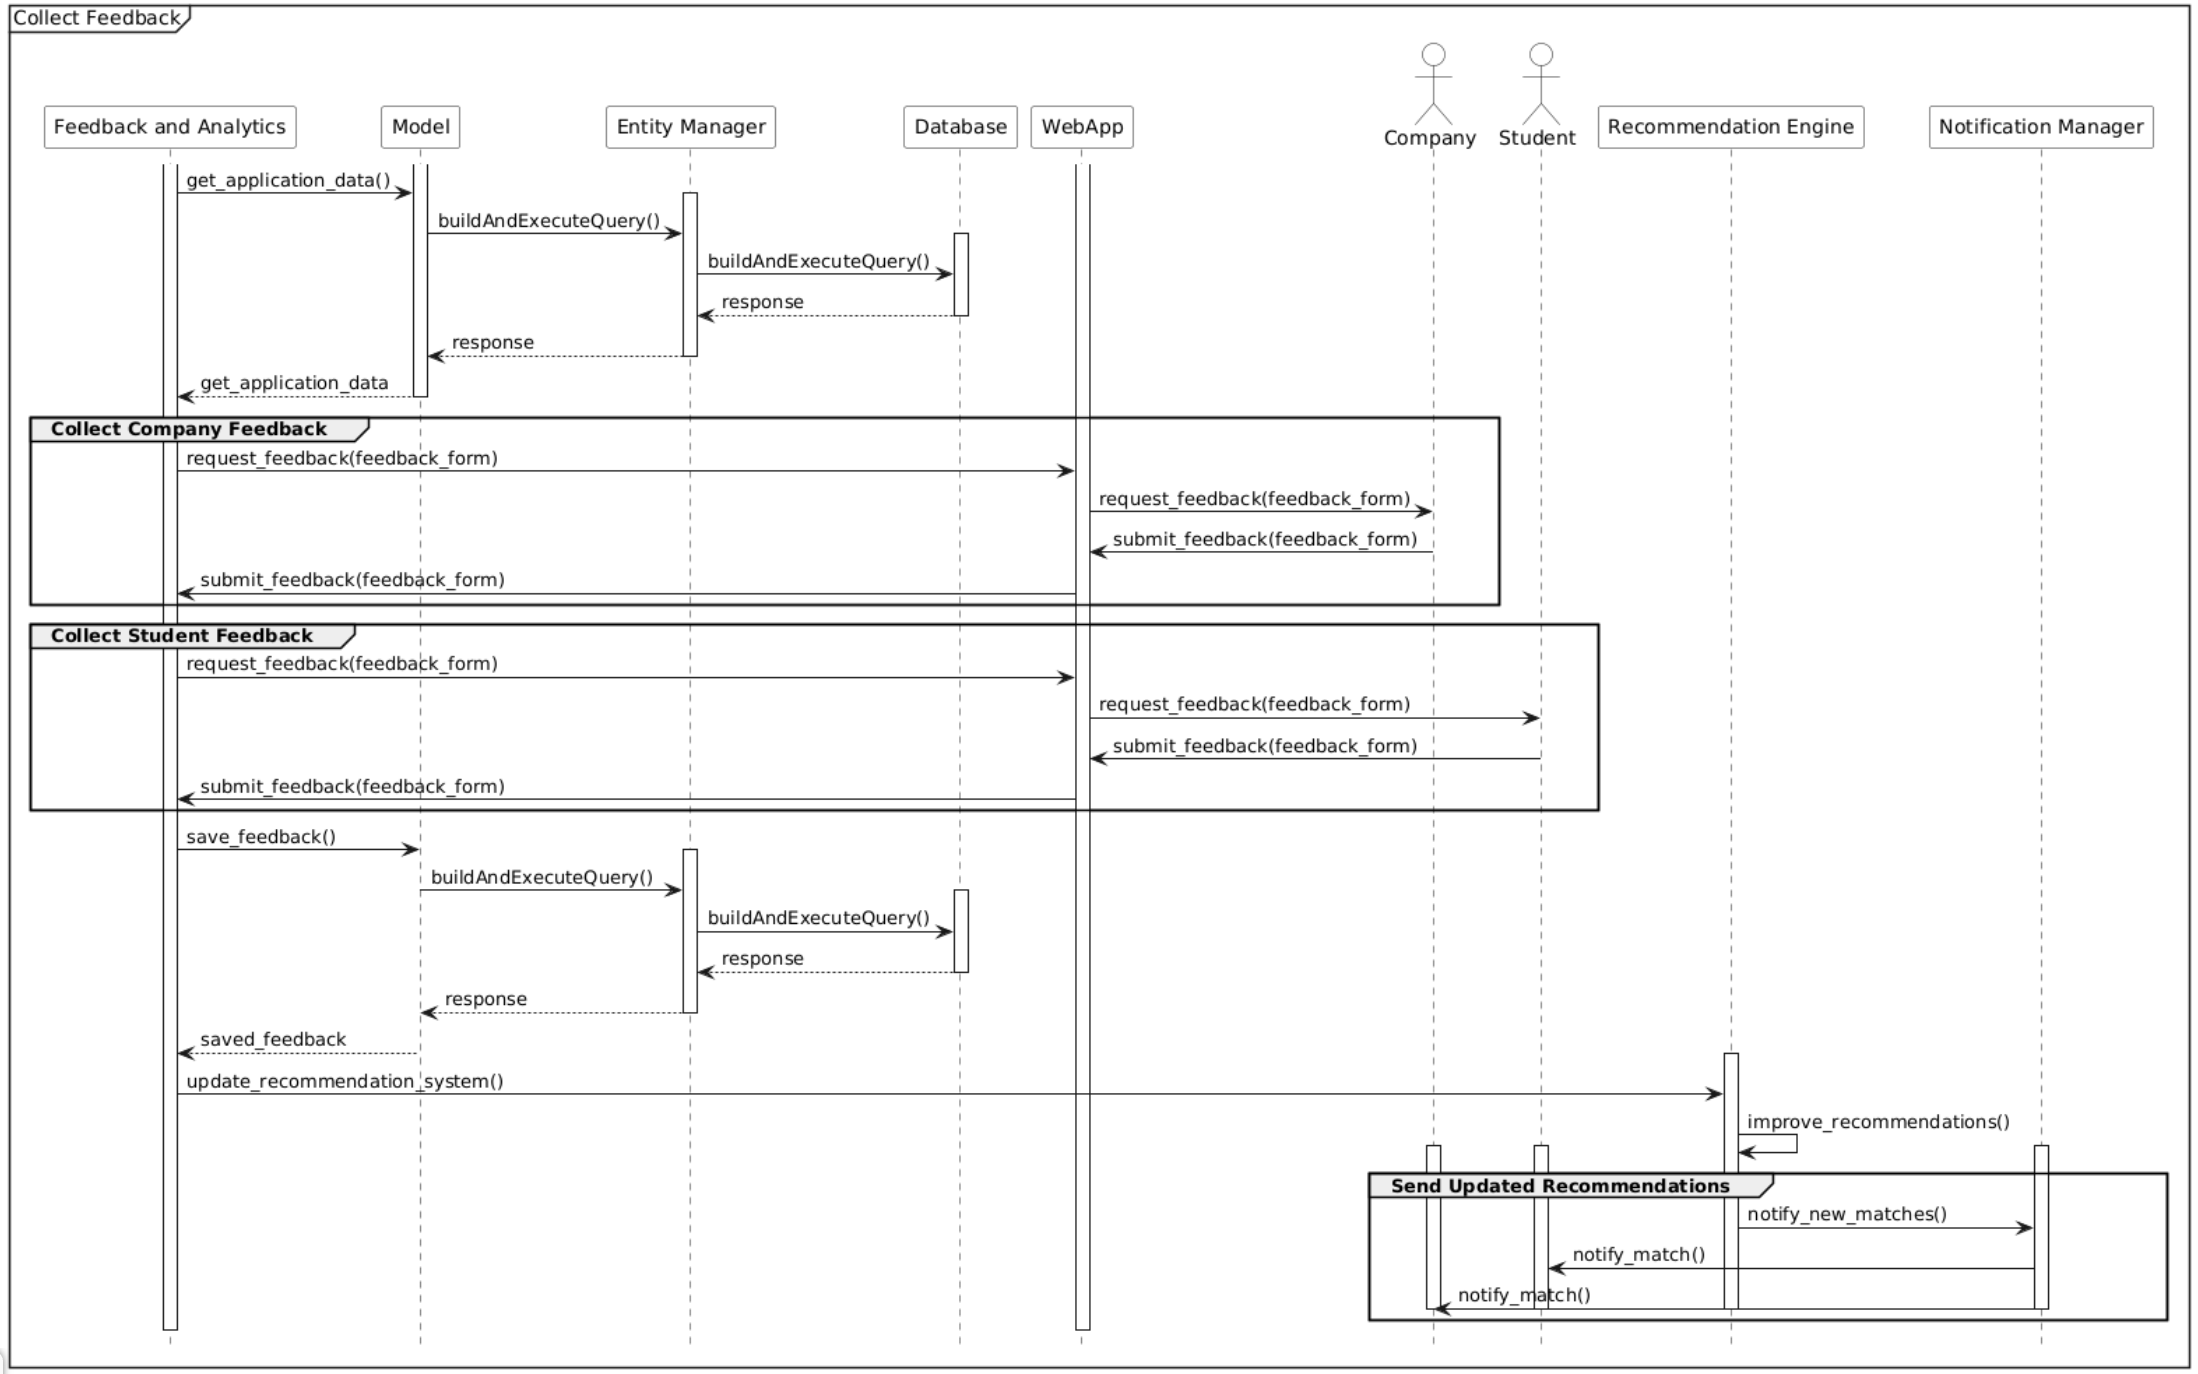
\includegraphics[width=0.8\textwidth]{Images/Collect Feedback sequence diagram.png}
    \caption{\label{fig:metamodel9}[UC15] Collect Feedback Sequence Diagram}
    \end{figure}
    \clearpage
    \item \textbf{Monitor Internship Status} \\ \\
    Users can monitor the internship status. University can monitor internships of it's students. After login university administrator can go to university's profile page and from there can see the list of their students. For each students university administrator can get the internship details and progress from database which is handled by Internship Monitor Manager. The following diagram is the runtime sequence diagram for the Internship Monitor Manage Sequence Diagram use case.
    \begin{figure}[H]
    \centering
    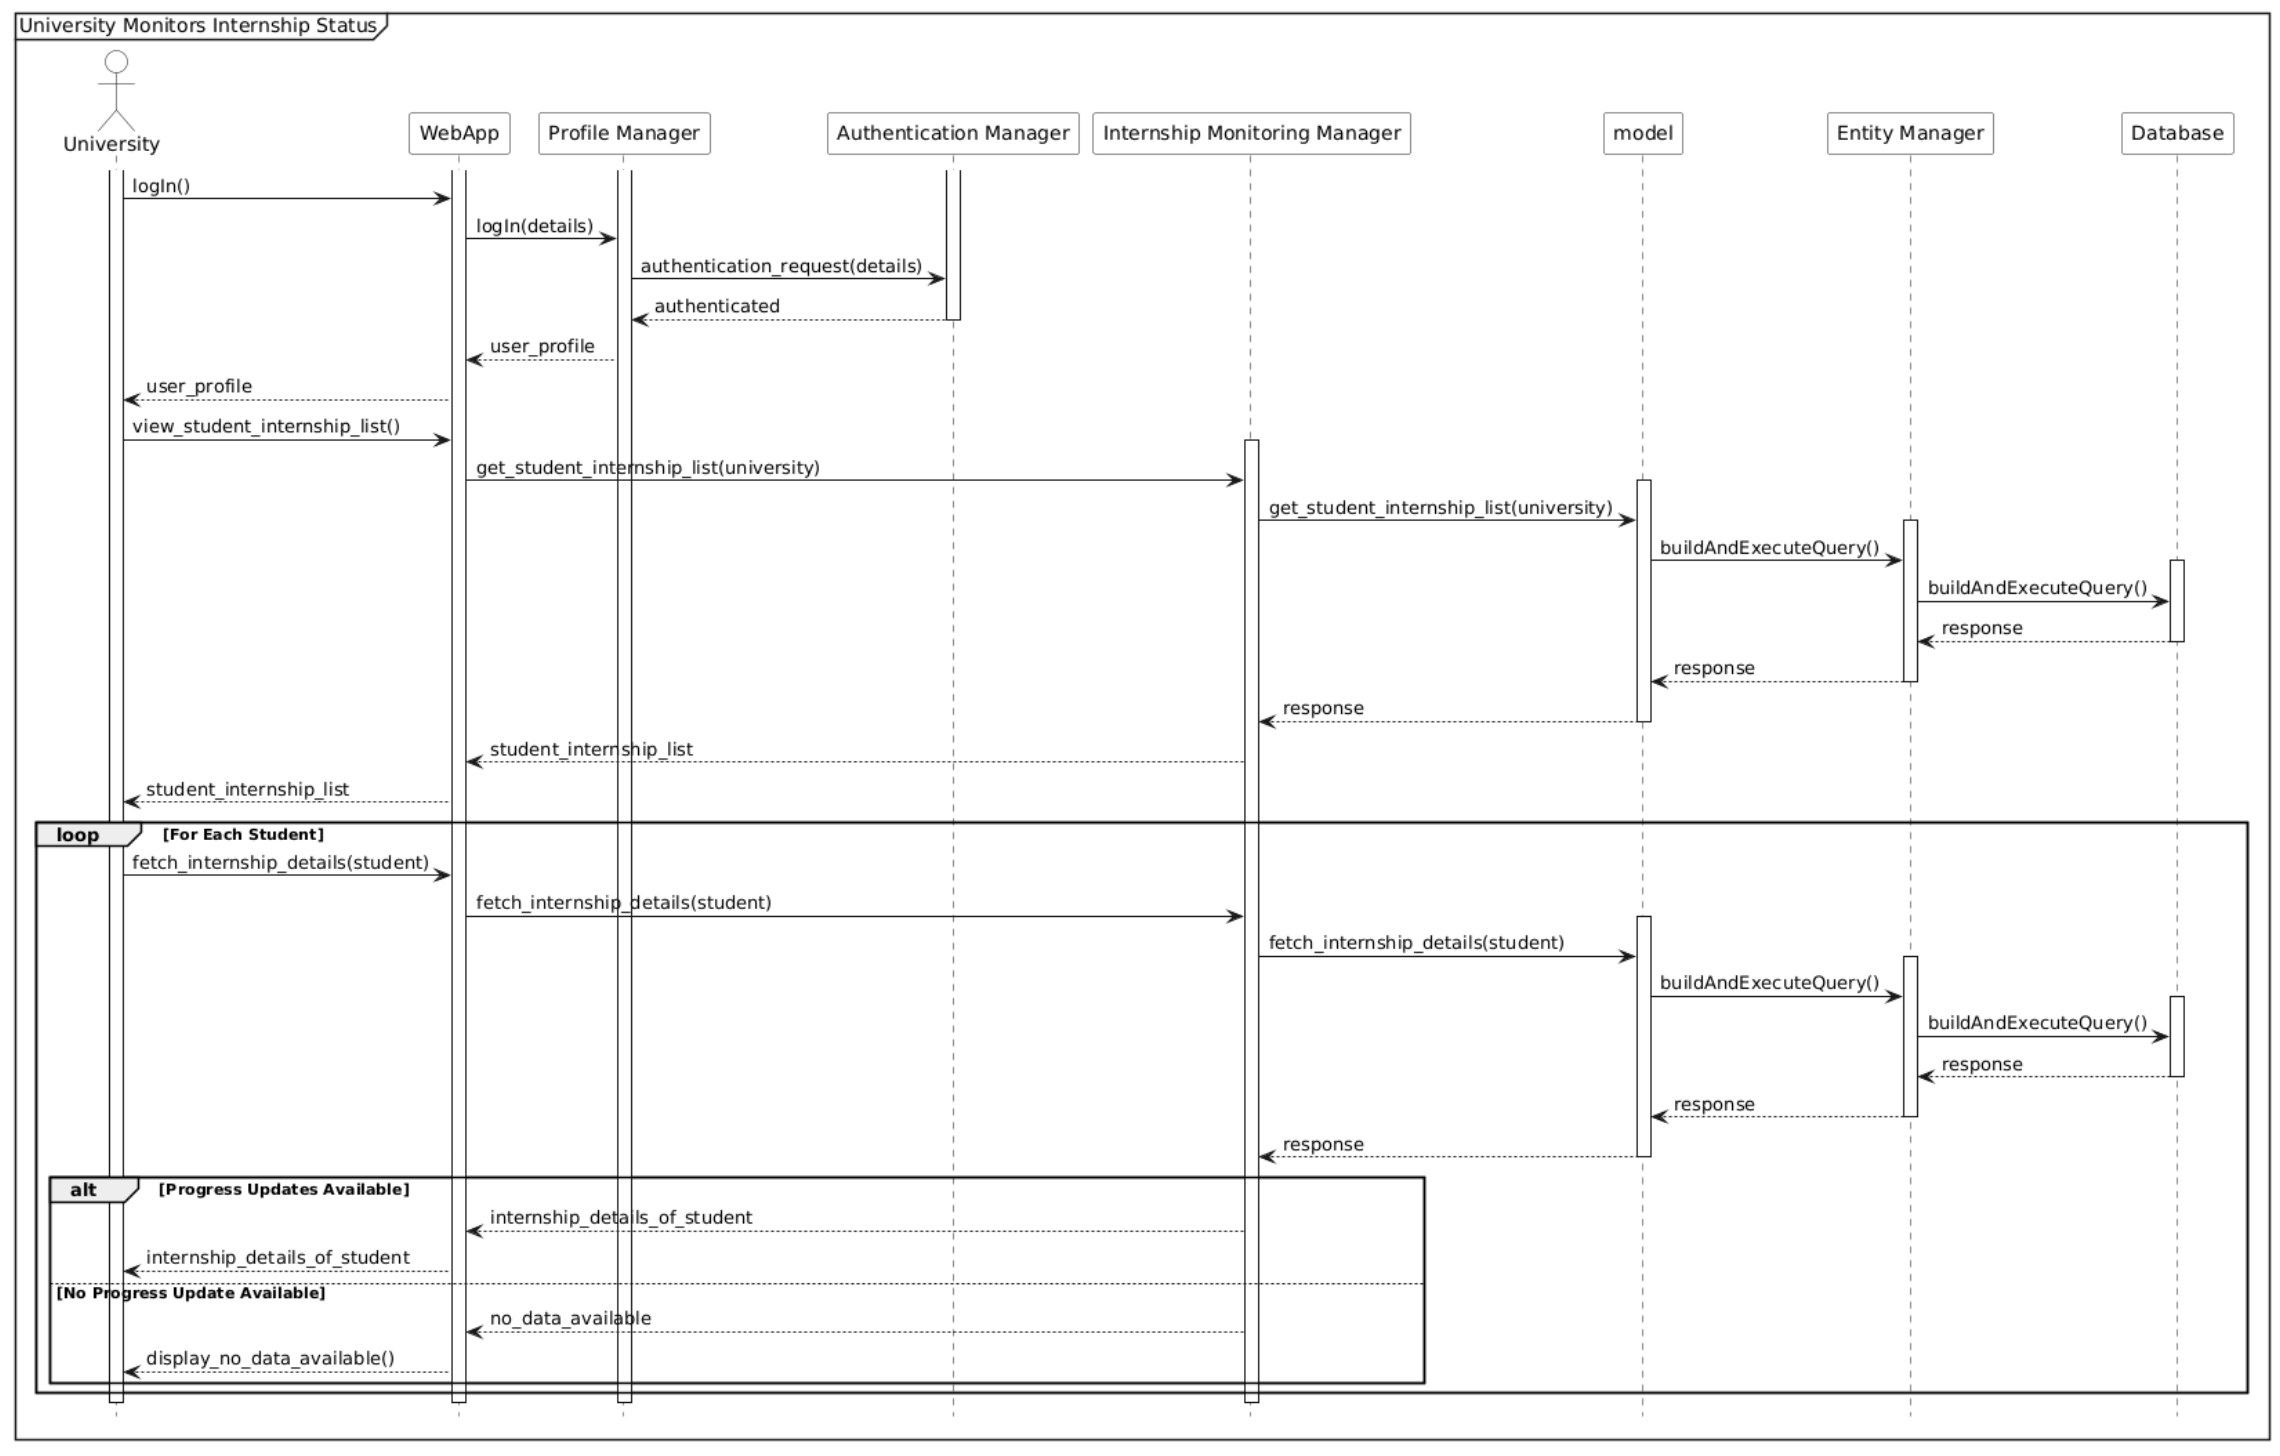
\includegraphics[width=0.8\textwidth]{Images/Uni_monitors_internship_status_sequence_diag.png}
    \caption{\label{fig:metamodel9}[UC16] Monitor Internship Status Sequence Diagram}
    \end{figure}
    \item \textbf{Handle Complaints and Issues} \\ \\
    University can login in to the S\&C web application then click on show complaints. It will fetch complaints through the Complaints Manager. If any complaints exist, university can take any decision which will be notified to the students and then mark the complaint as "Resolved" for flag for further actions required. In both the cases the complaint status and details will be updated in the database. The following diagram is the runtime sequence diagram for the Handle Complaints and Issues Sequence Diagram use case.
    \begin{figure}[H]
    \centering
    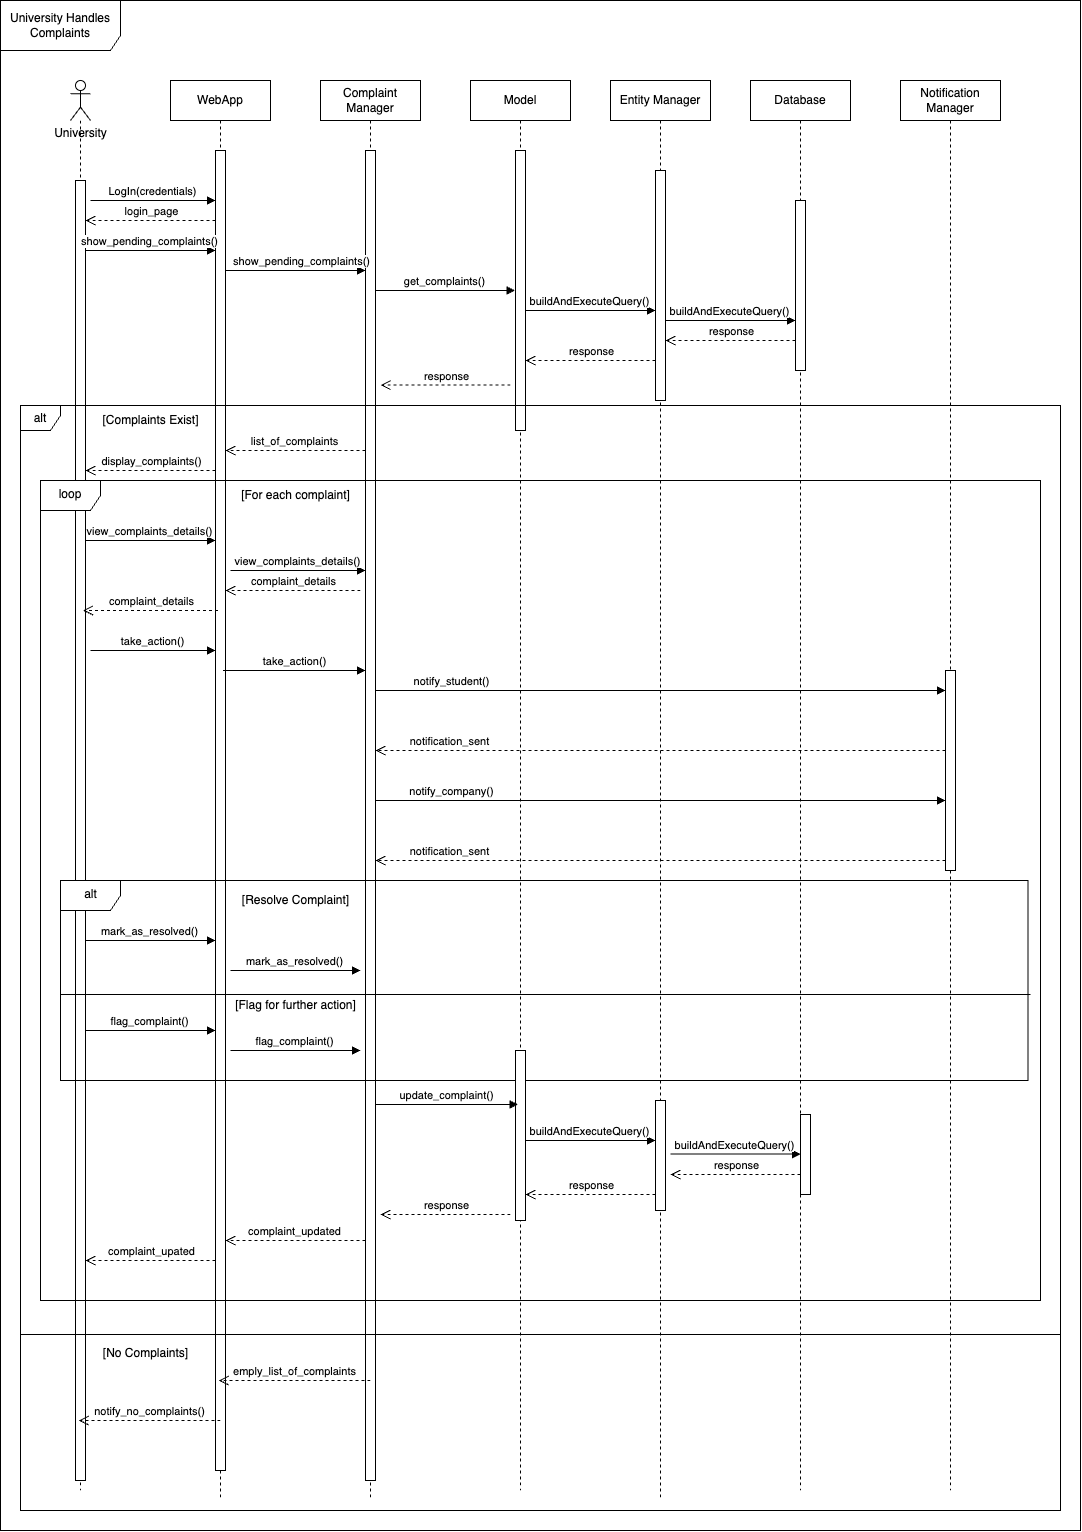
\includegraphics[width=0.8\textwidth]{Images/Uni_handles_complaints.png}
    \caption{\label{fig:metamodel9}[UC17] University Handles Complaints Sequence Diagram}
    \end{figure}
\end{itemize}

% 
\clearpage
\subsection{Component interfaces}

In this section as to represent Component interfaces we are representing API endpoints. The main focus is on the methods used, the
parameters required and on the responses.\\ 

\begin{figure}[H]
\centering
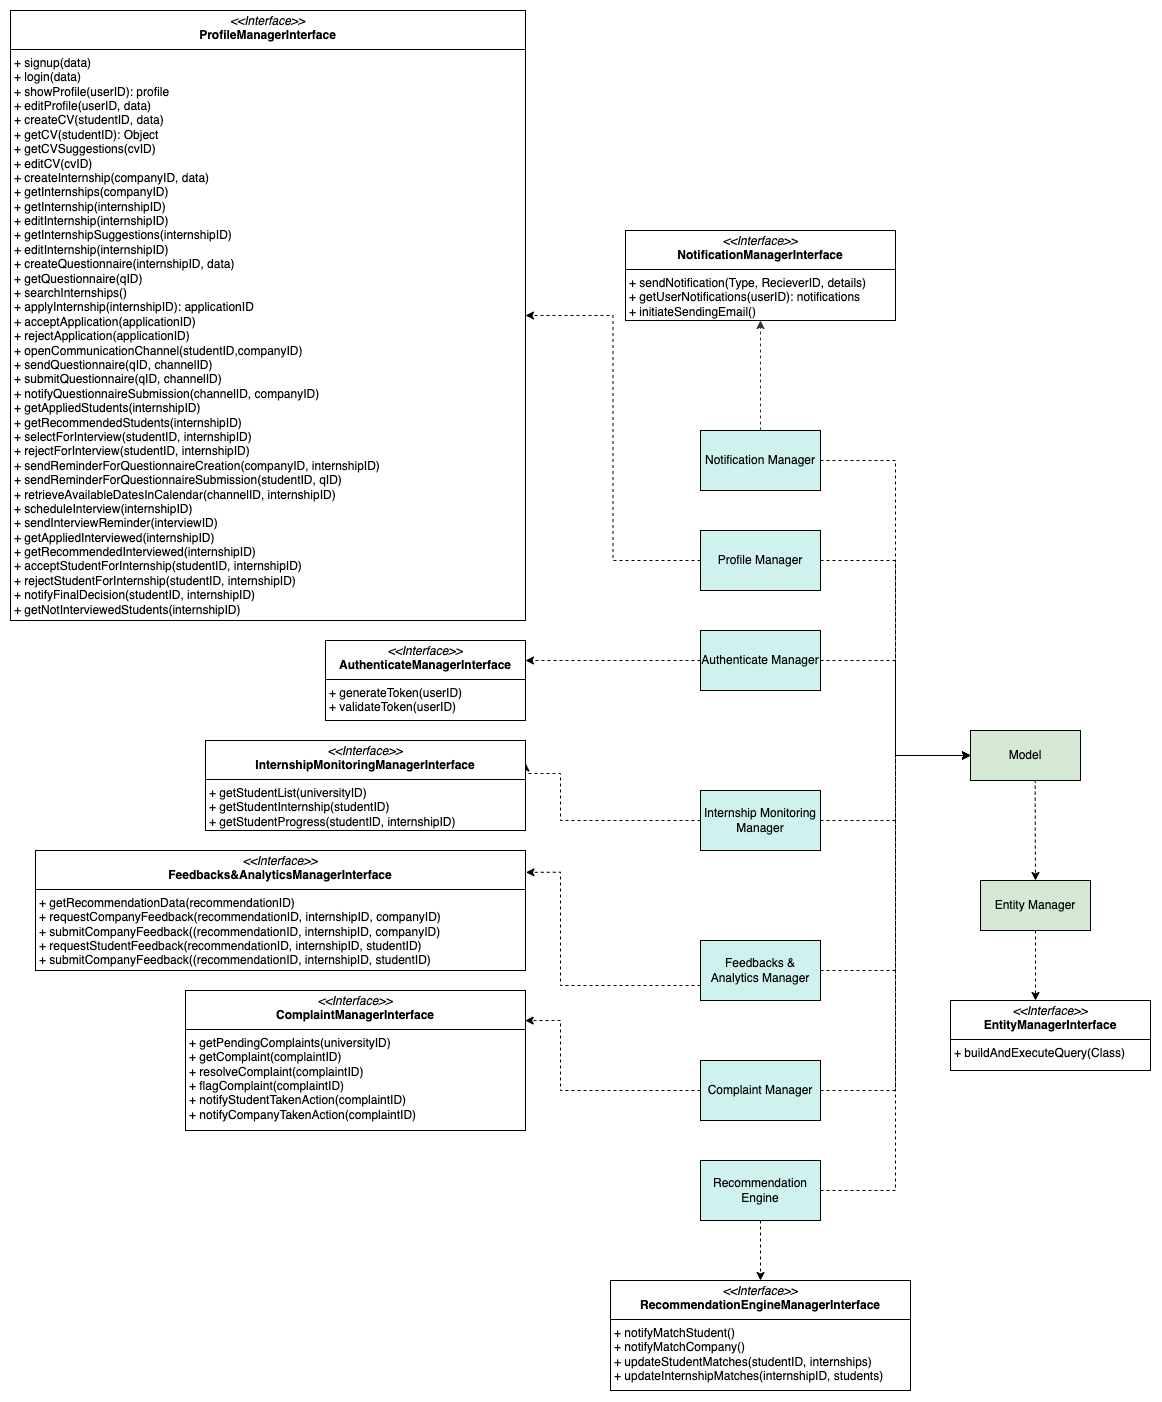
\includegraphics[width=0.8\textwidth]{Images/component_interfaces_class_diagram.png}
\caption{\label{fig:metamodel4} Component Interfaces Class Diagram}
\end{figure}

\subsubsection{API Endpoints}

\begin{itemize}
    \item \textbf{POST /api/users/signup}  
    \begin{itemize}
        \item \textbf{Description:} Registers a new user.
        \item \textbf{Request Body:} \texttt{\{ name, email, password, role, ...\}}
        \item \textbf{Response:}
        \begin{itemize}
            \item 201 Created: \texttt{\{ userId \}}
            \item 400 Bad Request: Validation errors.
        \end{itemize}
    \end{itemize}

    \item \textbf{POST /api/users/login}  
    \begin{itemize}
        \item \textbf{Description:} Logs in an existing user.
        \item \textbf{Request Body:} \texttt{\{ email, password \}}
        \item \textbf{Response:}
        \begin{itemize}
            \item 200 OK: \texttt{\{ token, userDetails \}}
            \item 401 Unauthorized: Invalid credentials.
        \end{itemize}
    \end{itemize}

    \item \textbf{GET /api/users/profile/\{userId\}}  
    \begin{itemize}
        \item \textbf{Description:} Fetches the profile of a user.
        \item \textbf{Path Parameters:} \texttt{userId}
        \item \textbf{Response:}
        \begin{itemize}
            \item 200 OK: \texttt{\{ userProfile \}}
            \item 404 Not Found: User does not exist.
        \end{itemize}
    \end{itemize}

    \item \textbf{PUT /api/users/editprofile/\{userId\}}  
    \begin{itemize}
        \item \textbf{Description:} Updates the profile of a user.
        \item \textbf{Request Body:} \texttt{\{ profileUpdates \}}
        \item \textbf{Response:}
        \begin{itemize}
            \item 200 OK: \texttt{\{ success: true \}}
            \item 400 Bad Request: Validation errors.
        \end{itemize}
    \end{itemize}

    \item \textbf{POST /api/cv/create}  
    \begin{itemize}
        \item \textbf{Description:} Creates a CV for a student.
        \item \textbf{Request Body:} \texttt{\{ studentId, cvDetails \}}
        \item \textbf{Response:}
        \begin{itemize}
            \item 201 Created: \texttt{\{ cvId \}}
            \item 400 Bad Request: Validation errors.
        \end{itemize}
    \end{itemize}
    
    \item \textbf{GET /api/cv/getcv/\{studentId\}}  
    \begin{itemize}
        \item \textbf{Description:} Retrieves the CV of a specific student.
        \item \textbf{Path Parameters:} \texttt{studentId}
        \item \textbf{Response:}
        \begin{itemize}
            \item 200 OK: \texttt{\{ cvDetails \}}
            \item 404 Not Found: No CV found for the specified student.
        \end{itemize}
    \end{itemize}

    \item \textbf{POST /api/cv/suggestions/\{studentId\}}  
    \begin{itemize}
        \item \textbf{Description:} Requests suggestions for improving a specific student's CV.
        \item \textbf{Path Parameters:} \texttt{studentId}
        \item \textbf{Request Body:} \texttt{\{ details: [...] \}}
        \item \textbf{Response:}
        \begin{itemize}
            \item 200 OK: \texttt{\{ suggestions: [...] \}}
            \item 404 Not Found: CV not found for the specified student.
            \item 400 Bad Request: Validation errors.
        \end{itemize}
    \end{itemize}

    \item \textbf{POST /api/cv/edit/\{cvId\}}  
    \begin{itemize}
        \item \textbf{Description:} Allows a student to edit an existing CV.
        \item \textbf{Path Parameters:} \texttt{cvId}
        \item \textbf{Request Body:} \texttt{\{ updatedCvDetails \}}
        \item \textbf{Response:}
        \begin{itemize}
            \item 200 OK: \texttt{\{ success: true, message: "CV updated successfully." \}}
            \item 404 Not Found: No CV found with the specified \texttt{cvId}.
            \item 400 Bad Request: Validation errors in the provided CV details.
        \end{itemize}
    \end{itemize}


    \item \textbf{POST /api/companies/internships/create/\{companyId\}}  
    \begin{itemize}
        \item \textbf{Description:} Creates a new internship posting for a specific company.
        \item \textbf{Path Parameters:} \texttt{companyId}
        \item \textbf{Request Body:} \texttt{\{ title, description, requirements \}}
        \item \textbf{Response:}
        \begin{itemize}
            \item 201 Created: \texttt{\{ internshipId \}}
            \item 400 Bad Request: Validation errors.
        \end{itemize}
    \end{itemize}
    
    \item \textbf{GET /api/companies/internships/\{companyId\}}  
    \begin{itemize}
        \item \textbf{Description:} Retrieves a list of internships for a specific company.
        \item \textbf{Path Parameters:} \texttt{companyId}
        \item \textbf{Query Parameters:} \texttt{\{ filterOptions \}}
        \item \textbf{Response:}
        \begin{itemize}
            \item 200 OK: \texttt{\{ internships: [...] \}}
            \item 401 Unauthorized: Access denied.
        \end{itemize}
    \end{itemize}

    \item \textbf{GET /api/internships/details/\{internshipId\}}  
    \begin{itemize}
        \item \textbf{Description:} Retrieves detailed information about a specific internship.
        \item \textbf{Path Parameters:} \texttt{internshipId}
        \item \textbf{Response:}
        \begin{itemize}
            \item 200 OK: \texttt{\{ internshipDetails: { ... } \}}
            \item 404 Not Found: No internship found with the specified \texttt{internshipId}.
            \item 400 Bad Request: Invalid internship ID.
        \end{itemize}
    \end{itemize}


    \item \textbf{POST /api/companies/internships/suggestions/\{companyId\}/\{internshipId\}} 
    \begin{itemize}
        \item \textbf{Description:} Requests suggestions for improving a specific internship post created by a specific company.
        \item \textbf{Path Parameters:} \texttt{companyId}, \texttt{internshipId}
        \item \textbf{Request Body:} \texttt{\{ details: [...] \}}
        \item \textbf{Response:}
        \begin{itemize}
            \item 200 OK: \texttt{\{ suggestions: [...] \}}
            \item 404 Not Found: Internship not found for the specified company.
            \item 400 Bad Request: Validation errors.
        \end{itemize}
    \end{itemize}


    \item \textbf{POST /api/internships/edit/\{internshipId\}}  
    \begin{itemize}
        \item \textbf{Description:} Allows a company to edit an existing internship posting.
        \item \textbf{Path Parameters:} \texttt{internshipId}
        \item \textbf{Request Body:} \texttt{\{ updatedInternshipDetails \}}
        \item \textbf{Response:}
        \begin{itemize}
            \item 200 OK: \texttt{\{ success: true, message: "Internship updated successfully." \}}
            \item 404 Not Found: No internship found with the specified \texttt{internshipId}.
            \item 400 Bad Request: Validation errors in the provided internship details.
        \end{itemize}
    \end{itemize}


    
    \item \textbf{POST /api/internships/questionnaire/\{internshipId\}}  
    \begin{itemize}
        \item \textbf{Description:} Creates a questionnaire for an internship.
        \item \textbf{Request Body:} \texttt{\{ questions: [...], internshipId \}}
        \item \textbf{Response:}
        \begin{itemize}
            \item 201 Created: \texttt{\{ questionnaireId \}}
            \item 400 Bad Request: Validation errors.
        \end{itemize}
    \end{itemize}
    
    \item \textbf{GET /api/internships/questionnaire/\{internshipId\}}  
    \begin{itemize}
        \item \textbf{Description:} Retrieves the questionnaire for an internship.
        \item \textbf{Path Parameters:} \texttt{internshipId}
        \item \textbf{Response:}
        \begin{itemize}
            \item 200 OK: \texttt{\{ questionnaireDetails \}}
            \item 404 Not Found: Questionnaire not found.
        \end{itemize}
    \end{itemize}

    \item \textbf{POST /api/notifications/student/matches/\{studentId\}}  
    \begin{itemize}
        \item \textbf{Description:} Sends a notification to a student about matching internships found.
        \item \textbf{Path Parameters:} studentId  
        \item \textbf{Request Body:} 
        \texttt{\{ 
            "matches": [...] 
        \}}
        \item \textbf{Response:}
        \begin{itemize}
            \item 200 OK: \texttt{\{ success: true, message: "Notification sent to student." \}}
            \item 404 Not Found: Student not found.
            \item 500 Internal Server Error: Notification sending failed.
        \end{itemize}
    \end{itemize}


    \item \textbf{POST /api/notifications/company/matches/\{companyId\}}  
    \begin{itemize}
        \item \textbf{Description:} Sends a notification to a company about matching students found for an internship.
        \item \textbf{Path Parameters:} companyId  
        \item \textbf{Request Body:} 
        \texttt{\{ 
            "matches": [...] 
        \}}
        \item \textbf{Response:}
        \begin{itemize}
            \item 200 OK: \texttt{\{ success: true, message: "Notification sent to company." \}}
            \item 404 Not Found: Company not found.
            \item 500 Internal Server Error: Notification sending failed.
        \end{itemize}
    \end{itemize}

    \item \textbf{POST /api/dashboards/student/update-matches\{studentId\}}  
    \begin{itemize}
        \item \textbf{Description:} Updates a student's dashboard with the latest matches found by the recommendation engine.
        \item \textbf{Path Parameters:} studentId  
        \item \textbf{Request Body:} 
        \texttt{\{ 
            "matches": [...] 
        \}}
        \item \textbf{Response:}
        \begin{itemize}
            \item 200 OK: \texttt{\{ success: true, message: "Dashboard updated successfully." \}}
            \item 404 Not Found: Student not found.
            \item 500 Internal Server Error: Dashboard update failed.
        \end{itemize}
    \end{itemize}

    \item \textbf{POST /api/dashboards/company/update-matches/\{companyId\}}  
    \begin{itemize}
        \item \textbf{Description:} Updates a company's dashboard with the latest matches found by the recommendation engine.
        \item \textbf{Path Parameters:} companyId  
        \item \textbf{Request Body:} 
        \texttt{\{ 
            "matches": [...] 
        \}}
        \item \textbf{Response:}
        \begin{itemize}
            \item 200 OK: \texttt{\{ success: true, message: "Dashboard updated successfully." \}}
            \item 404 Not Found: Company not found.
            \item 500 Internal Server Error: Dashboard update failed.
        \end{itemize}
    \end{itemize}

    \item \textbf{GET /api/internships/search}  
    \begin{itemize}
        \item \textbf{Description:} Allows a student to search for internships based on specified criterias.
        \item \textbf{Request Body:} A JSON object containing the search criteria.
        \item \textbf{Response:}
        \begin{itemize}
            \item 200 OK: \texttt{\{ internships: [...] \}}
            \begin{itemize}
                \item Returns a list of internships that match the given criteria.
            \end{itemize}
            \item 400 Bad Request: Validation errors in the provided criteria.
            \item 401 Unauthorized: User is not authenticated.
        \end{itemize}
    \end{itemize}


    \item \textbf{POST /api/internships/apply/\{internshipId\}}  
    \begin{itemize}
        \item \textbf{Description:} Allows a student to apply to a specific internship.
        \item \textbf{Request Body:} A JSON object containing the application details.
        \item \textbf{Path Parameters:}  
        \begin{itemize}
            \item \texttt{internshipId}: The ID of the internship the student is applying to.
        \end{itemize}
        \item \textbf{Response:}
        \begin{itemize}
            \item 200 OK: \texttt{\{ success: true, message: "Application submitted successfully." \}}
            \item 400 Bad Request: Validation errors in the application details.
            \item 401 Unauthorized: User is not authenticated.
            \item 404 Not Found: Internship not found.
        \end{itemize}
    \end{itemize}


    \item \textbf{POST /api/internships/applications/accept/\{internshipId\}/\{applicationId\}}  
    \begin{itemize}
        \item \textbf{Description:} Allows a company to accept a student's application for a specific internship.
        \item \textbf{Path Parameters:}  
        \begin{itemize}
            \item \texttt{internshipId}: The ID of the internship the application belongs to.
            \item \texttt{applicationId}: The ID of the student's application.
        \end{itemize}
        \item \textbf{Response:}
        \begin{itemize}
            \item 200 OK: \texttt{\{ success: true, message: "Application accepted successfully." \}}
            \item 400 Bad Request: Validation errors or missing data.
            \item 401 Unauthorized: User is not authenticated or authorized.
            \item 404 Not Found: Internship or application not found.
        \end{itemize}
    \end{itemize}

    \item \textbf{POST /api/internships/applications/reject/\{internshipId\}/\{applicationId\}}  
    \begin{itemize}
        \item \textbf{Description:} Allows a company to reject a student's application for a specific internship.
        \item \textbf{Path Parameters:} internshipId, applicationId  
        \item \textbf{Response:}
        \begin{itemize}
            \item 200 OK: \texttt{\{ success: true, message: "Application rejected successfully." \}}
            \item 400 Bad Request: Validation errors or missing data.
            \item 401 Unauthorized: User is not authenticated or authorized.
            \item 404 Not Found: Internship or application not found.
        \end{itemize}
    \end{itemize}


    \item \textbf{POST /api/communication/open/\{studentId\}/\{companyId\}}  
    \begin{itemize}
        \item \textbf{Description:} Opens a communication channel between a student and a company during the selection process.
        \item \textbf{Path Parameters:} studentId, companyId  
        \item \textbf{Response:}
        \begin{itemize}
            \item 200 OK: \texttt{\{ success: true, message: "Communication channel opened successfully." \}}
            \item 400 Bad Request: Validation errors in the request.
            \item 401 Unauthorized: User is not authenticated.
        \end{itemize}
    \end{itemize}


    \item \textbf{POST /api/questionnaire/send/\{qId\}/\{studentId\}/\{internshipId\}/\{channelId\}}  
    \begin{itemize}
        \item \textbf{Description:} Sends a questionnaire from the company to a student as part of the selection process.
        \item \textbf{Path Parameters:} studentId, internshipId, channelId, qId  
        \item \textbf{Request Body:} 
        \texttt{\{ 
            "questions": ["string", "string", ...]
        \}}
        \item \textbf{Response:}
        \begin{itemize}
            \item 200 OK: \texttt{\{ success: true, message: "Questionnaire sent successfully." \}}
            \item 404 Not Found: Internship or student not found.
            \item 400 Bad Request: Validation errors in the request body.
        \end{itemize}
    \end{itemize}

    \item \textbf{POST /api/questionnaire/submit//\{qId\}\{studentId\}/\{internshipId\}/\{channelId\}}  
    \begin{itemize}
        \item \textbf{Description:} Allows a student to submit answers to a received questionnaire.
        \item \textbf{Path Parameters:} studentId, internshipId, channelId, qId 
        \item \textbf{Request Body:} 
        \texttt{\{ 
            "answers": ["string", "string", ...] 
        \}}
        \item \textbf{Response:}
        \begin{itemize}
            \item 200 OK: \texttt{\{ success: true, message: "Answers submitted successfully." \}}
            \item 404 Not Found: Questionnaire not found.
            \item 400 Bad Request: Validation errors in the answers.
        \end{itemize}
    \end{itemize}

    \item \textbf{POST /api/questionnaire/notify/\{channelId\}/\{companyId\}/\{internshipId\}}  
    \begin{itemize}
        \item \textbf{Description:} Notifies the company when a questionnaire has been submitted by the student.
        \item \textbf{Path Parameters:} channelId, companyId, internshipId  
        \item \textbf{Response:}
        \begin{itemize}
            \item 200 OK: \texttt{\{ success: true, message: "Notification sent successfully." \}}
            \item 500 Internal Server Error: Failed to send the notification.
        \end{itemize}
    \end{itemize}

    \item \textbf{GET /api/internships/applied-students/\{internshipId\}}  
    \begin{itemize}
        \item \textbf{Description:} Retrieves a list of students who applied for a specific internship.
        \item \textbf{Path Parameters:} \texttt{internshipId}
        \item \textbf{Response:}
        \begin{itemize}
            \item 200 OK: \texttt{\{ students: [...] \}}
            \item 404 Not Found: No internship found with the specified \texttt{internshipId}, or no students applied.
            \item 400 Bad Request: Invalid internship ID.
        \end{itemize}
    \end{itemize}


    \item \textbf{GET /api/internships/recommended-students/\{internshipId\}}  
    \begin{itemize}
        \item \textbf{Description:} Retrieves a list of students recommended by the system for a specific internship.
        \item \textbf{Path Parameters:} \texttt{internshipId}
        \item \textbf{Response:}
        \begin{itemize}
            \item 200 OK: \texttt{\{ recommendedStudents: [...] \}}
            \item 404 Not Found: No internship found with the specified \texttt{internshipId}, or no recommended students available.
            \item 400 Bad Request: Invalid internship ID.
        \end{itemize}
    \end{itemize}



    \item \textbf{POST /api/interviews/select/\{studentId\}/\{internshipId\}}  
    \begin{itemize}
        \item \textbf{Description:} Adds a student to the interview shortlist for a specific internship.
        \item \textbf{Path Parameters:} studentId, internshipId  
        \item \textbf{Response:}
        \begin{itemize}
            \item 200 OK: \texttt{\{ success: true, message: "Student added to interview shortlist." \}}
            \item 404 Not Found: Internship or student not found.
            \item 400 Bad Request: Validation errors in the request.
        \end{itemize}
    \end{itemize}



    \item \textbf{POST /api/interviews/reject/\{studentId\}/\{internshipId\}}  
    \begin{itemize}
        \item \textbf{Description:} Rejects a student for a specific internship and removes them from the selection process.
        \item \textbf{Path Parameters:} studentId, internshipId  
        \item \textbf{Response:}
        \begin{itemize}
            \item 200 OK: \texttt{\{ success: true, message: "Student rejected successfully." \}}
            \item 404 Not Found: Internship or student not found.
            \item 400 Bad Request: Validation errors in the request.
        \end{itemize}
    \end{itemize}

    \item \textbf{POST /api/questionnaire/reminder/\{studentId\}/\{internshipId\}}  
    \begin{itemize}
        \item \textbf{Description:} Sends a reminder to the student about an incomplete questionnaire.
        \item \textbf{Path Parameters:} studentId, internshipId  
        \item \textbf{Response:}
        \begin{itemize}
            \item 200 OK: \texttt{\{ success: true, message: "Reminder sent successfully." \}}
            \item 404 Not Found: Questionnaire not found.
            \item 500 Internal Server Error: Failed to send the reminder.
        \end{itemize}
    \end{itemize}

    \item \textbf{POST /api/questionnaire/reminder/\{studentId\}/\{qId\}}  
    \begin{itemize}
        \item \textbf{Description:} Sends a reminder to a student to complete and submit a specific questionnaire.
        \item \textbf{Path Parameters:} \texttt{studentId}, \texttt{qId}
        \item \textbf{Response:}
        \begin{itemize}
            \item 200 OK: \texttt{\{ success: true, message: "Reminder sent successfully." \}}
            \item 404 Not Found: Student or questionnaire not found with the specified IDs.
            \item 400 Bad Request: Invalid student ID or questionnaire ID.
            \item 500 Internal Server Error: Failed to send the reminder.
        \end{itemize}
    \end{itemize}


    \item \textbf{GET /api/interviews/calendar/\{internshipId\}/\{channelId\}}  
    \begin{itemize}
        \item \textbf{Description:} Retrieves available dates and times for scheduling an interview.
        \item \textbf{Path Parameters:} internshipId, channelId
        \item \textbf{Response:}
        \begin{itemize}
            \item 200 OK: \texttt{\{ availableDates: [ "YYYY-MM-DD HH:mm", ... ] \}}
            \item 400 Bad Request: Invalid internship ID or unavailable calendar data.
            \item 401 Unauthorized: User is not authenticated.
        \end{itemize}
    \end{itemize}

    \item \textbf{POST /api/interviews/schedule/\{internshipId\}}  
    \begin{itemize}
        \item \textbf{Description:} Schedules an interview for a specific internship by providing date, time, and meeting link details in the student's and company's dashboard.
        \item \textbf{Path Parameters:} 
        \begin{itemize}
            \item \texttt{internshipId}: The ID of the internship for which the interview is being scheduled.
        \end{itemize}
        \item \textbf{Request Body:} 
        \texttt{\{ 
            "date": "YYYY-MM-DD", 
            "time": "HH:mm", 
            "meetingLink": "string" 
        \}}
        \item \textbf{Response:}
        \begin{itemize}
            \item 200 OK: \texttt{\{ success: true, message: "Interview scheduled successfully." \}}
            \item 400 Bad Request: Invalid date, time, or missing meeting link.
            \item 404 Not Found: Internship not found.
            \item 401 Unauthorized: User is not authenticated.
        \end{itemize}
    \end{itemize}


    \item \textbf{POST /api/interviews/notify/\{interviewId\}}  
    \begin{itemize}
        \item \textbf{Description:} Sends notifications to the student and the company about the scheduled interview.
        \item \textbf{Path Parameters:} interviewId
        \item \textbf{Request Body:} 
        \texttt{\{ 
            "message": "string"
        \}}
        \item \textbf{Response:}
        \begin{itemize}
            \item 200 OK: \texttt{\{ success: true, message: "Notifications sent successfully." \}}
            \item 404 Not Found: Interview ID not found.
            \item 500 Internal Server Error: Failed to send notifications.
        \end{itemize}
    \end{itemize}


    \item \textbf{POST /api/interviews/reminder/\{interviewId\}}  
    \begin{itemize}
        \item \textbf{Description:} Sends reminders to both the student and company before the interview.
        \item \textbf{Path Parameters:} 
        \begin{itemize}
            \item \texttt{interviewId}: The ID of the interview for which reminders will be sent.
        \end{itemize}
        \item \textbf{Response:}
        \begin{itemize}
            \item 200 OK: \texttt{\{ success: true, message: "Reminders sent successfully." \}}
            \item 404 Not Found: Interview ID not found.
            \item 500 Internal Server Error: Failed to send reminders.
        \end{itemize}
    \end{itemize}

    \item \textbf{GET /api/internships/interviewed-applied-students/\{internshipId\}}  
    \begin{itemize}
        \item \textbf{Description:} Retrieves a list of students who were interviewed and had applied for a specific internship.
        \item \textbf{Path Parameters:} internshipId  
        \item \textbf{Response:}
        \begin{itemize}
            \item 200 OK: \texttt{\{ students: [...] \}}
            \item 404 Not Found: Internship not found.
            \item 400 Bad Request: Invalid internship ID.
        \end{itemize}
    \end{itemize}

    \item \textbf{GET /api/internships/interviewed-recommended-students/\{internshipId\}}  
    \begin{itemize}
        \item \textbf{Description:} Retrieves a list of students who were interviewed based on the system's recommendations for a specific internship.
        \item \textbf{Path Parameters:} internshipId  
        \item \textbf{Response:}
        \begin{itemize}
            \item 200 OK: \texttt{\{ students: [...] \}}
            \item 404 Not Found: Internship not found.
            \item 400 Bad Request: Invalid internship ID.
        \end{itemize}
    \end{itemize}

    \item \textbf{POST /api/internships/accept/\{internshipId\}/\{studentId\}}  
    \begin{itemize}
        \item \textbf{Description:} Accepts a student for a specific internship and notifies them.
        \item \textbf{Path Parameters:} internshipId, studentId  
        \item \textbf{Response:}
        \begin{itemize}
            \item 200 OK: \texttt{\{ success: true, message: "Student accepted and notified." \}}
            \item 404 Not Found: Internship or student not found.
            \item 400 Bad Request: Invalid parameters.
        \end{itemize}
    \end{itemize}

    \item \textbf{POST /api/internships/reject/\{internshipId\}/\{studentId\}}  
    \begin{itemize}
        \item \textbf{Description:} Rejects a student for a specific internship and notifies them.
        \item \textbf{Path Parameters:} internshipId, studentId  
        \item \textbf{Response:}
        \begin{itemize}
            \item 200 OK: \texttt{\{ success: true, message: "Student rejected and notified." \}}
            \item 404 Not Found: Internship or student not found.
            \item 400 Bad Request: Invalid parameters.
        \end{itemize}
    \end{itemize}

    \item \textbf{POST /api/internships/notify/\{internshipId\}/\{studentId\}}  
    \begin{itemize}
        \item \textbf{Description:} notifies the student of the final decision for a specific student in the context of an internship (either accept or reject).
        \item \textbf{Path Parameters:} internshipId, studentId  
        \item \textbf{Request Body:} 
        \texttt{\{ 
            "message": "string"
        \}}
        \item \textbf{Response:}
        \begin{itemize}
            \item 200 OK: \texttt{\{ success: true, message: "Final decision notified." \}}
            \item 404 Not Found: Internship or student not found.
            \item 400 Bad Request: Invalid decision or parameters.
        \end{itemize}
    \end{itemize}

    \item \textbf{GET /api/internships/no-interviewed-students/\{internshipId\}}  
    \begin{itemize}
        \item \textbf{Description:} Checks if there are no interviewed students left for finalization in a specific internship.
        \item \textbf{Path Parameters:} internshipId  
        \item \textbf{Response:}
        \begin{itemize}
            \item 200 OK: \texttt{\{ noStudents: true | false \}}
            \item 404 Not Found: Internship not found.
            \item 400 Bad Request: Invalid internship ID.
        \end{itemize}
    \end{itemize}


    \item \textbf{GET /api/recommendations/data/\{recommendationId\}}  
    \begin{itemize}
        \item \textbf{Description:} Retrieves detailed data about a specific recommendation.
        \item \textbf{Path Parameters:} recommendationId  
        \item \textbf{Response:}
        \begin{itemize}
            \item 200 OK: \texttt{\{ recommendationData: { ... } \}}
            \item 404 Not Found: Recommendation not found.
            \item 400 Bad Request: Invalid recommendation ID.
        \end{itemize}
    \end{itemize}

    \item \textbf{POST /api/feedback/request/company/\{internshipId\}/\{companyId\}/\{recommendationId\}}  
    \begin{itemize}
        \item \textbf{Description:} Sends a request to the company for feedback on a specific recommendation.
        \item \textbf{Path Parameters:} internshipId, companyId, recommendationId  
        \item \textbf{Response:}
        \begin{itemize}
            \item 200 OK: \texttt{\{ success: true, message: "Feedback request sent to the company." \}}
            \item 404 Not Found: Internship, company, or recommendation not found.
            \item 400 Bad Request: Invalid recommendation ID.
        \end{itemize}
    \end{itemize}

    \item \textbf{POST /api/feedback/submit/company/\{internshipId\}/\{companyId\}/\{recommendationId\}}  
    \begin{itemize}
        \item \textbf{Description:} Allows a company to submit feedback on a specific recommendation.
        \item \textbf{Path Parameters:} internshipId, companyId, recommendationId  
        \item \textbf{Request Body:} 
        \texttt{\{ 
            "feedback": Object
        \}}
        \item \textbf{Response:}
        \begin{itemize}
            \item 200 OK: \texttt{\{ success: true, message: "Feedback submitted successfully." \}}
            \item 404 Not Found: Internship, company, or recommendation not found.
            \item 400 Bad Request: Validation errors in the feedback.
        \end{itemize}
    \end{itemize}

    \item \textbf{POST /api/feedback/request/student/\{internshipId\}/\{studentId\}/\{recommendationId\}}  
    \begin{itemize}
        \item \textbf{Description:} Sends a request to a student for feedback on a specific recommendation.
        \item \textbf{Path Parameters:} internshipId, studentId, recommendationId  
        \item \textbf{Response:}
        \begin{itemize}
            \item 200 OK: \texttt{\{ success: true, message: "Feedback request sent to the student." \}}
            \item 404 Not Found: Internship, student, or recommendation not found.
            \item 400 Bad Request: Invalid recommendation ID.
        \end{itemize}
    \end{itemize}


    \item \textbf{POST /api/feedback/submit/student/\{internshipId\}/\{studentId\}/\{recommendationId\}}  
    \begin{itemize}
        \item \textbf{Description:} Allows a student to submit feedback on a specific recommendation.
        \item \textbf{Path Parameters:} internshipId, studentId, recommendationId  
        \item \textbf{Request Body:} 
        \texttt{\{ 
            "feedback": Object
        \}}
        \item \textbf{Response:}
        \begin{itemize}
            \item 200 OK: \texttt{\{ success: true, message: "Feedback submitted successfully." \}}
            \item 404 Not Found: Internship, student, or recommendation not found.
            \item 400 Bad Request: Validation errors in the feedback.
        \end{itemize}
    \end{itemize}

    \item \textbf{POST /api/feedback/save/\{recommendationId\}}  
    \begin{itemize}
        \item \textbf{Description:} Saves feedback provided by a student or company for a specific recommendation to the database.
        \item \textbf{Path Parameters:} recommendationId  
        \item \textbf{Request Body:} 
        \texttt{\{ 
            "feedback": Object
        \}}
        \item \textbf{Response:}
        \begin{itemize}
            \item 200 OK: \texttt{\{ success: true, message: "Feedback saved successfully." \}}
            \item 404 Not Found: Recommendation not found.
            \item 400 Bad Request: Validation errors in the feedback.
        \end{itemize}
    \end{itemize}

    \item \textbf{GET /api/internships/student-list/university/\{universityId\}}  
    \begin{itemize}
        \item \textbf{Description:} Retrieves a list of students and their internships associated with a specific university.
        \item \textbf{Path Parameters:} universityId  
        \item \textbf{Response:}
        \begin{itemize}
            \item 200 OK: \texttt{\{ students: [...] \}}
            \item 404 Not Found: University not found or no students associated.
            \item 400 Bad Request: Invalid university ID.
        \end{itemize}
    \end{itemize}

    \item \textbf{GET /api/internships/details/student/\{studentId\}}  
    \begin{itemize}
        \item \textbf{Description:} Retrieves detailed internship information for a specific student.
        \item \textbf{Path Parameters:} studentId  
        \item \textbf{Response:}
        \begin{itemize}
            \item 200 OK: \texttt{\{ internshipDetails: { ... } \}}
            \item 404 Not Found: Student or internship details not found.
            \item 400 Bad Request: Invalid student ID.
        \end{itemize}
    \end{itemize}

    \item \textbf{GET /api/internships/progress/student/\{studentId\}/\{internshipId\}}  
    \begin{itemize}
        \item \textbf{Description:} Retrieves progress updates for a student's internship.
        \item \textbf{Path Parameters:} studentId, internshipId
        \item \textbf{Response:}
        \begin{itemize}
            \item 200 OK: \texttt{\{ progressUpdates: [...] \}}
            \item 404 Not Found: No progress updates available for the student.
            \item 400 Bad Request: Invalid student ID.
        \end{itemize}
    \end{itemize}
    
    \item \textbf{GET /api/complaints/pending/university/\{universityId\}}  
    \begin{itemize}
        \item \textbf{Description:} Retrieves a list of pending complaints for the university.
        \item \textbf{Path Parameters:} universityId  
        \item \textbf{Response:}
        \begin{itemize}
            \item 200 OK: \texttt{\{ complaints: [...] \}}
            \item 404 Not Found: University or complaints not found.
            \item 400 Bad Request: Invalid university ID.
        \end{itemize}
    \end{itemize}

    \item \textbf{GET /api/complaints/details/\{complaintId\}}  
    \begin{itemize}
        \item \textbf{Description:} Retrieves the details of a specific complaint.
        \item \textbf{Path Parameters:} complaintId  
        \item \textbf{Response:}
        \begin{itemize}
            \item 200 OK: \texttt{\{ complaintDetails: { ... } \}}
            \item 404 Not Found: Complaint not found.
            \item 400 Bad Request: Invalid complaint ID.
        \end{itemize}
    \end{itemize}

    \item \textbf{POST /api/notifications/student/complaint/\{studentId\}/\{complaintId\}}  
    \begin{itemize}
        \item \textbf{Description:} Sends a notification to a student regarding the action taken on their complaint.
        \item \textbf{Path Parameters:} studentId, complaintId  
        \item \textbf{Response:}
        \begin{itemize}
            \item 200 OK: \texttt{\{ success: true, message: "Notification sent to student." \}}
            \item 404 Not Found: Student or complaint not found.
            \item 500 Internal Server Error: Failed to send notification.
        \end{itemize}
    \end{itemize}


    \item \textbf{POST /api/notifications/company/complaint/\{companyId\}/\{complaintId\}}  
    \begin{itemize}
        \item \textbf{Description:} Sends a notification to a company regarding the action taken on a complaint involving them.
        \item \textbf{Path Parameters:} companyId, complaintId  
        \item \textbf{Response:}
        \begin{itemize}
            \item 200 OK: \texttt{\{ success: true, message: "Notification sent to company." \}}
            \item 404 Not Found: Company or complaint not found.
            \item 500 Internal Server Error: Failed to send notification.
        \end{itemize}
    \end{itemize}

    \item \textbf{POST /api/complaints/resolve/\{complaintId\}}  
    \begin{itemize}
        \item \textbf{Description:} Marks a specific complaint as resolved.
        \item \textbf{Path Parameters:} complaintId  
        \item \textbf{Response:}
        \begin{itemize}
            \item 200 OK: \texttt{\{ success: true, message: "Complaint marked as resolved." \}}
            \item 404 Not Found: Complaint not found.
            \item 400 Bad Request: Invalid complaint ID.
        \end{itemize}
    \end{itemize}

    \item \textbf{POST /api/complaints/flag/\{complaintId\}}  
    \begin{itemize}
        \item \textbf{Description:} Flags a specific complaint for further action or investigation.
        \item \textbf{Path Parameters:} complaintId  
        \item \textbf{Response:}
        \begin{itemize}
            \item 200 OK: \texttt{\{ success: true, message: "Complaint flagged for further action." \}}
            \item 404 Not Found: Complaint not found.
            \item 400 Bad Request: Invalid complaint ID.
        \end{itemize}
    \end{itemize}

    \item \textbf{GET /api/notifications/\{userId\}}  
    \begin{itemize}
        \item \textbf{Description:} Retrieves notifications for a user.
        \item \textbf{Path Parameters:} \texttt{userId}
        \item \textbf{Response:}
        \begin{itemize}
            \item 200 OK: \texttt{\{ notifications: [...] \}}
            \item 401 Unauthorized: Access denied.
        \end{itemize}
    \end{itemize}

\end{itemize}
\subsection{Selected Architectural Styles and Patterns}

\subsubsection{Three-Tier Architecture}
The Three-Tier architecture divides the system into three logical layers: 
\begin{itemize}
    \item \textbf{Presentation Tier (Web Server):} This layer provides the user interface, typically through web pages or web applications. It is implemented using technologies like HTML, CSS, and JavaScript. This tier allows interaction between the user and the system.
    \item \textbf{Business Logic Tier (Application Server):} This layer acts as the intermediary, processing and implementing the business logic. It ensures the rules and workflows of the system are correctly executed. It is often responsible for making decisions and handling API requests.
    \item \textbf{Data Storage Tier (Database Server):} This is the backend layer responsible for managing and storing data. It runs on a Database Management System (DBMS), ensuring data persistence and security.
\end{itemize}
The Three-Tier architecture offers modularization, scalability, and separation of concerns, which simplifies maintenance and enhances control and security in the system.

\subsubsection{Model-View-Controller (MVC) Pattern}
The Model-View-Controller (MVC) pattern is adopted for its modular and maintainable software architecture. It is particularly well-suited for web applications:
\begin{itemize}
    \item \textbf{Model:} Manages the data, application logic, and rules of the system. It encapsulates the core functionality and ensures consistency in data handling.
    \item \textbf{View:} Represents the data visually to the users, such as charts, tables, or forms. Multiple views can exist for the same data, catering to different user needs.
    \item \textbf{Controller:} Acts as the intermediary between the Model and the View. It processes user inputs, communicates with the Model to fetch or manipulate data, and updates the View accordingly.
\end{itemize}
This pattern provides strong decoupling between the components, enhancing reliability, reusability, and clarity of the codebase. The distributed nature of this pattern supports scalable applications by efficiently handling user interfaces and data processing.

\subsubsection{RESTful APIs}
RESTful APIs (Representational State Transfer) are implemented to ensure seamless communication between the client and server. These APIs:
\begin{itemize}
    \item Use standard HTTP methods: GET, POST, PUT, DELETE, etc., for data exchange.
    \item Are stateless, ensuring each request is self-contained and independent of previous ones.
\end{itemize}
RESTful APIs are simple to implement, lightweight, and reduce server load, making them an ideal choice for scalable systems requiring smooth communication and data exchange.

\subsubsection{Cloud Hosted}
The S\&W is hosted on cloud and used third party cloud service providers for to manage and deliver services and applications. Some advantages of cloud deployment other than the already mentioned are as follows:
\begin{itemize}
    \item \textbf{High Availability:} Cloud providers offer uptime guarantees and data is often replicated across multiple data centers to ensure availability.
    \item \textbf{Security:} Cloud providers often implement strict security policies and invest heavily in infrastructure to protect data.
\end{itemize}
% \begin{itemize}
%     \item \textbf{High Availability: Cloud providers offer uptime guarantees and data is often replicated across multiple data centers to ensure availability.
%     \item \textbf{Security:} Cloud providers often implement strict security policies and invest heavily in infrastructure to protect data.
% \end{itemize}



\subsection{Other Design Decisions}

\subsubsection{Token-Based Authentication and Authorization}
The system employs a token-based authentication and authorization mechanism to secure access and maintain user sessions. Key features include:
\begin{itemize}
    \item \textbf{Token Generation:} Upon login, the server generates a unique token, such as a JWT (JSON Web Token), which is shared with the client.
    \item \textbf{Token Usage:} The token must be included in the header of every subsequent request requiring authentication or authorization.
    \item \textbf{Security Features:} Tokens are used for secure operations, such as identifying users, validating their roles, and safely sending sensitive data like email invitations.
\end{itemize}
This approach enhances security by ensuring only authenticated users can access restricted resources, while the stateless nature of tokens reduces the load on the server.

\subsubsection{Relational Database}
The system uses relational database for storing and querying of data. In relational database data is stored in a structured format using tables (called relations). This structure allows for easy querying, retrieval, and manipulation of data using a specialized query language, most commonly SQL. There are several upsides of using relational database, some of which are as follows:
\begin{itemize}
\item \textbf{Structured Data Storage:} Data is stored in a highly organized and logical manner, which makes it easy to access, manage, and update.
\item \textbf{Scalability:} Relational databases can handle large volumes of data and can scale horizontally or vertically to accommodate more records or users.
\item \textbf{Flexible Queries:} It provides powerful querying capabilities, allowing retrieval and manipulation of data in complex ways. 

\end{itemize}







%------------------------------------------------------------------------------------------------------------------------------------------------
\clearpage
{\color{Blue}{\section{User Interface Design}}}
\label{sect:userinterface}

\begin{figure}[!htb]
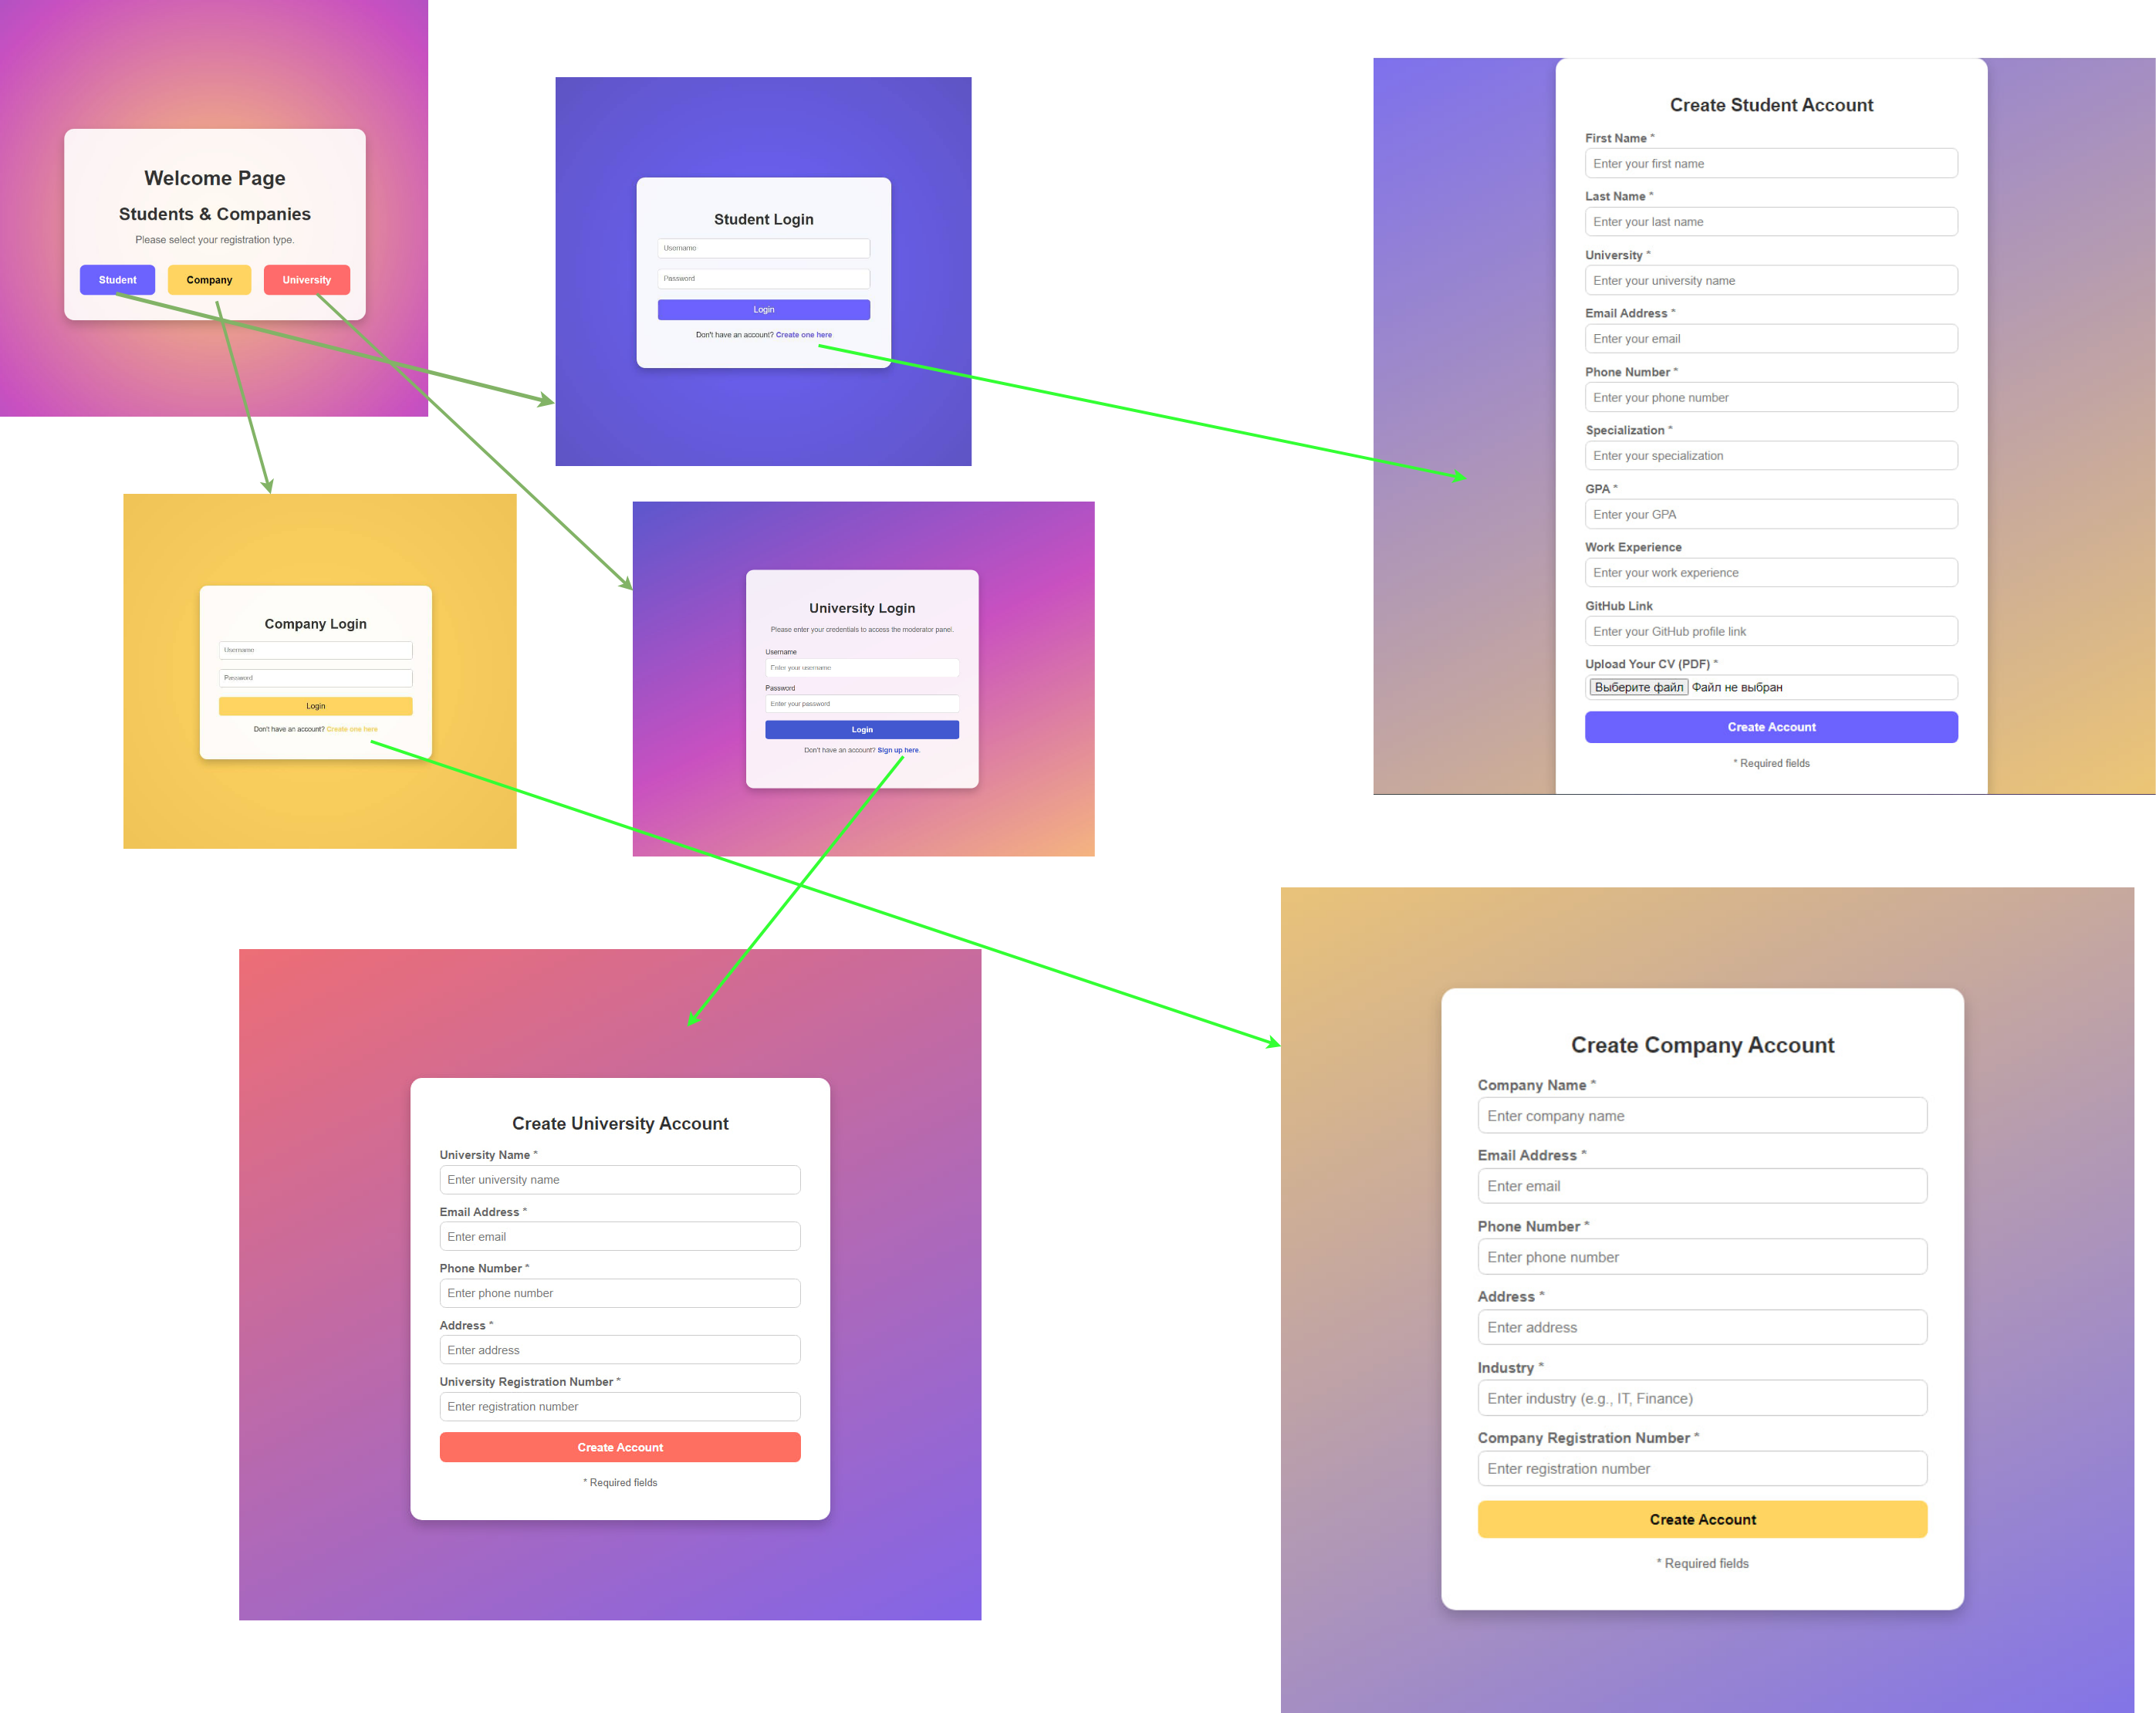
\includegraphics[width=\textwidth, angle=0]{Images/Main1.png}
\caption{\label{fig:metamodel}User Journey from starting page and Navigation Flow for Students, Companies, and Universities on the Platform.}
\end{figure}

\begin{figure}[!h]
\centering
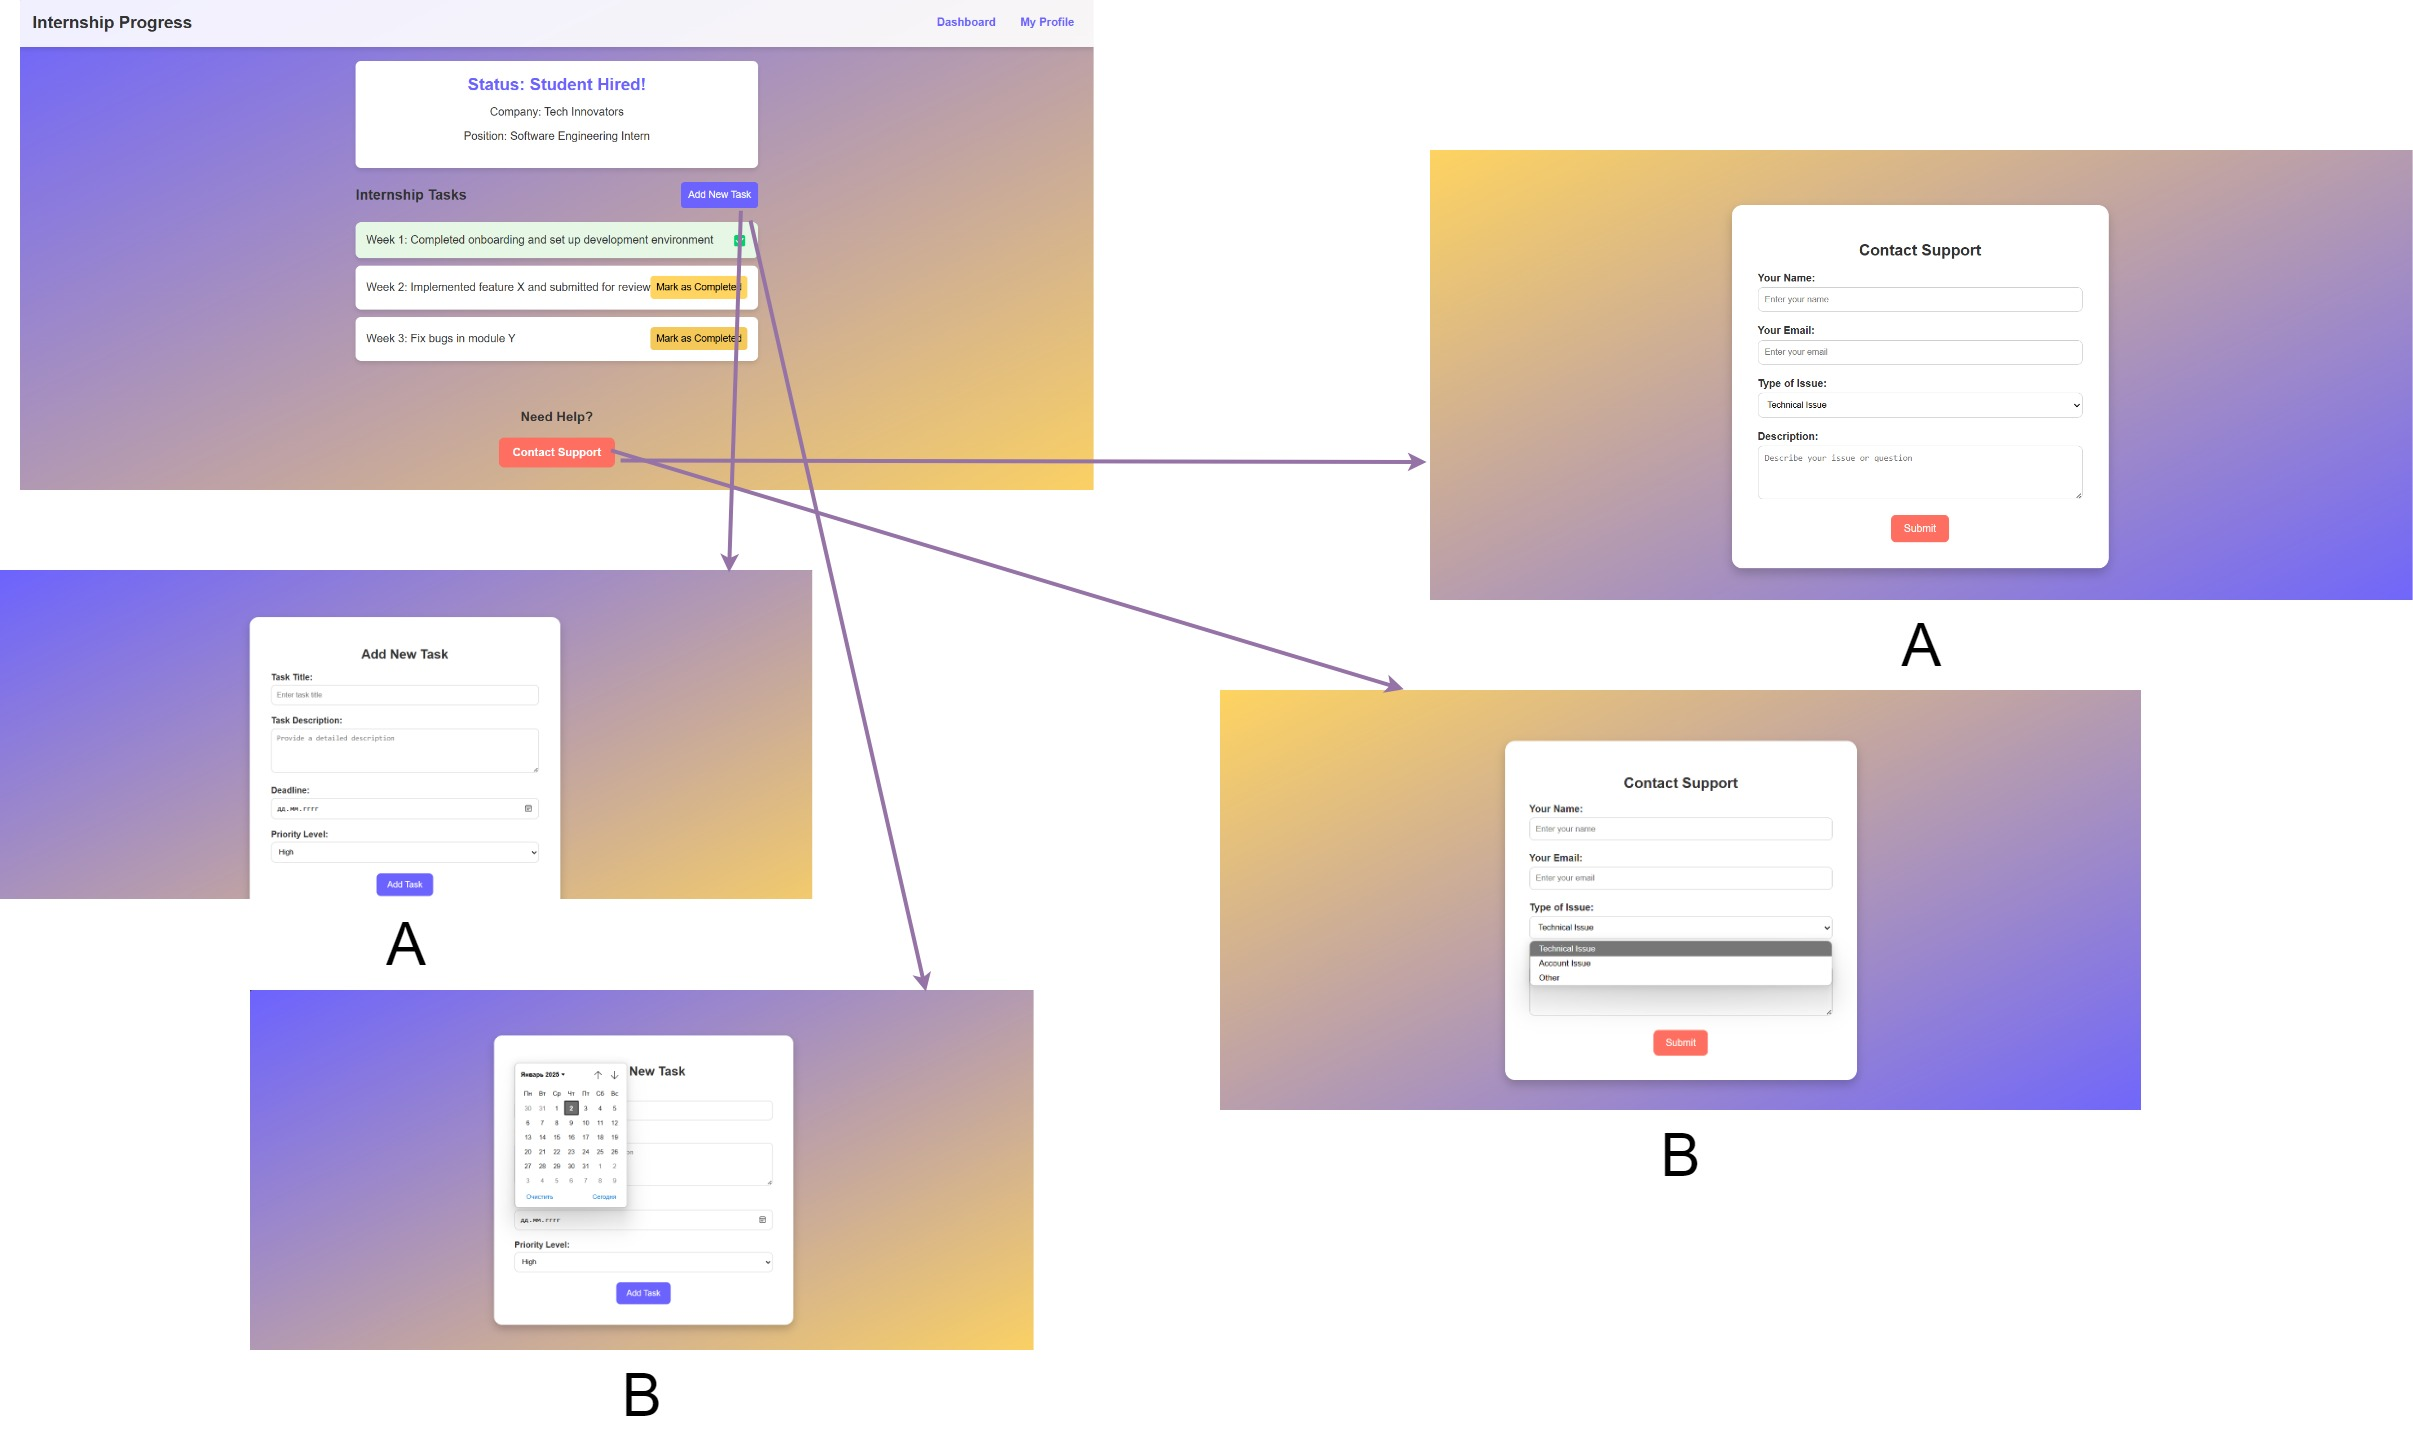
\includegraphics[width=0.9\textwidth, angle=0]{Images/Main2.jpg}
\caption{\label{fig:metamodel}Internship Progress and Task Management Flow: Users can track their internship progress, add new tasks (A), and contact support (B) for assistance with various issues.}
\end{figure}

\begin{figure}[!h]
\centering
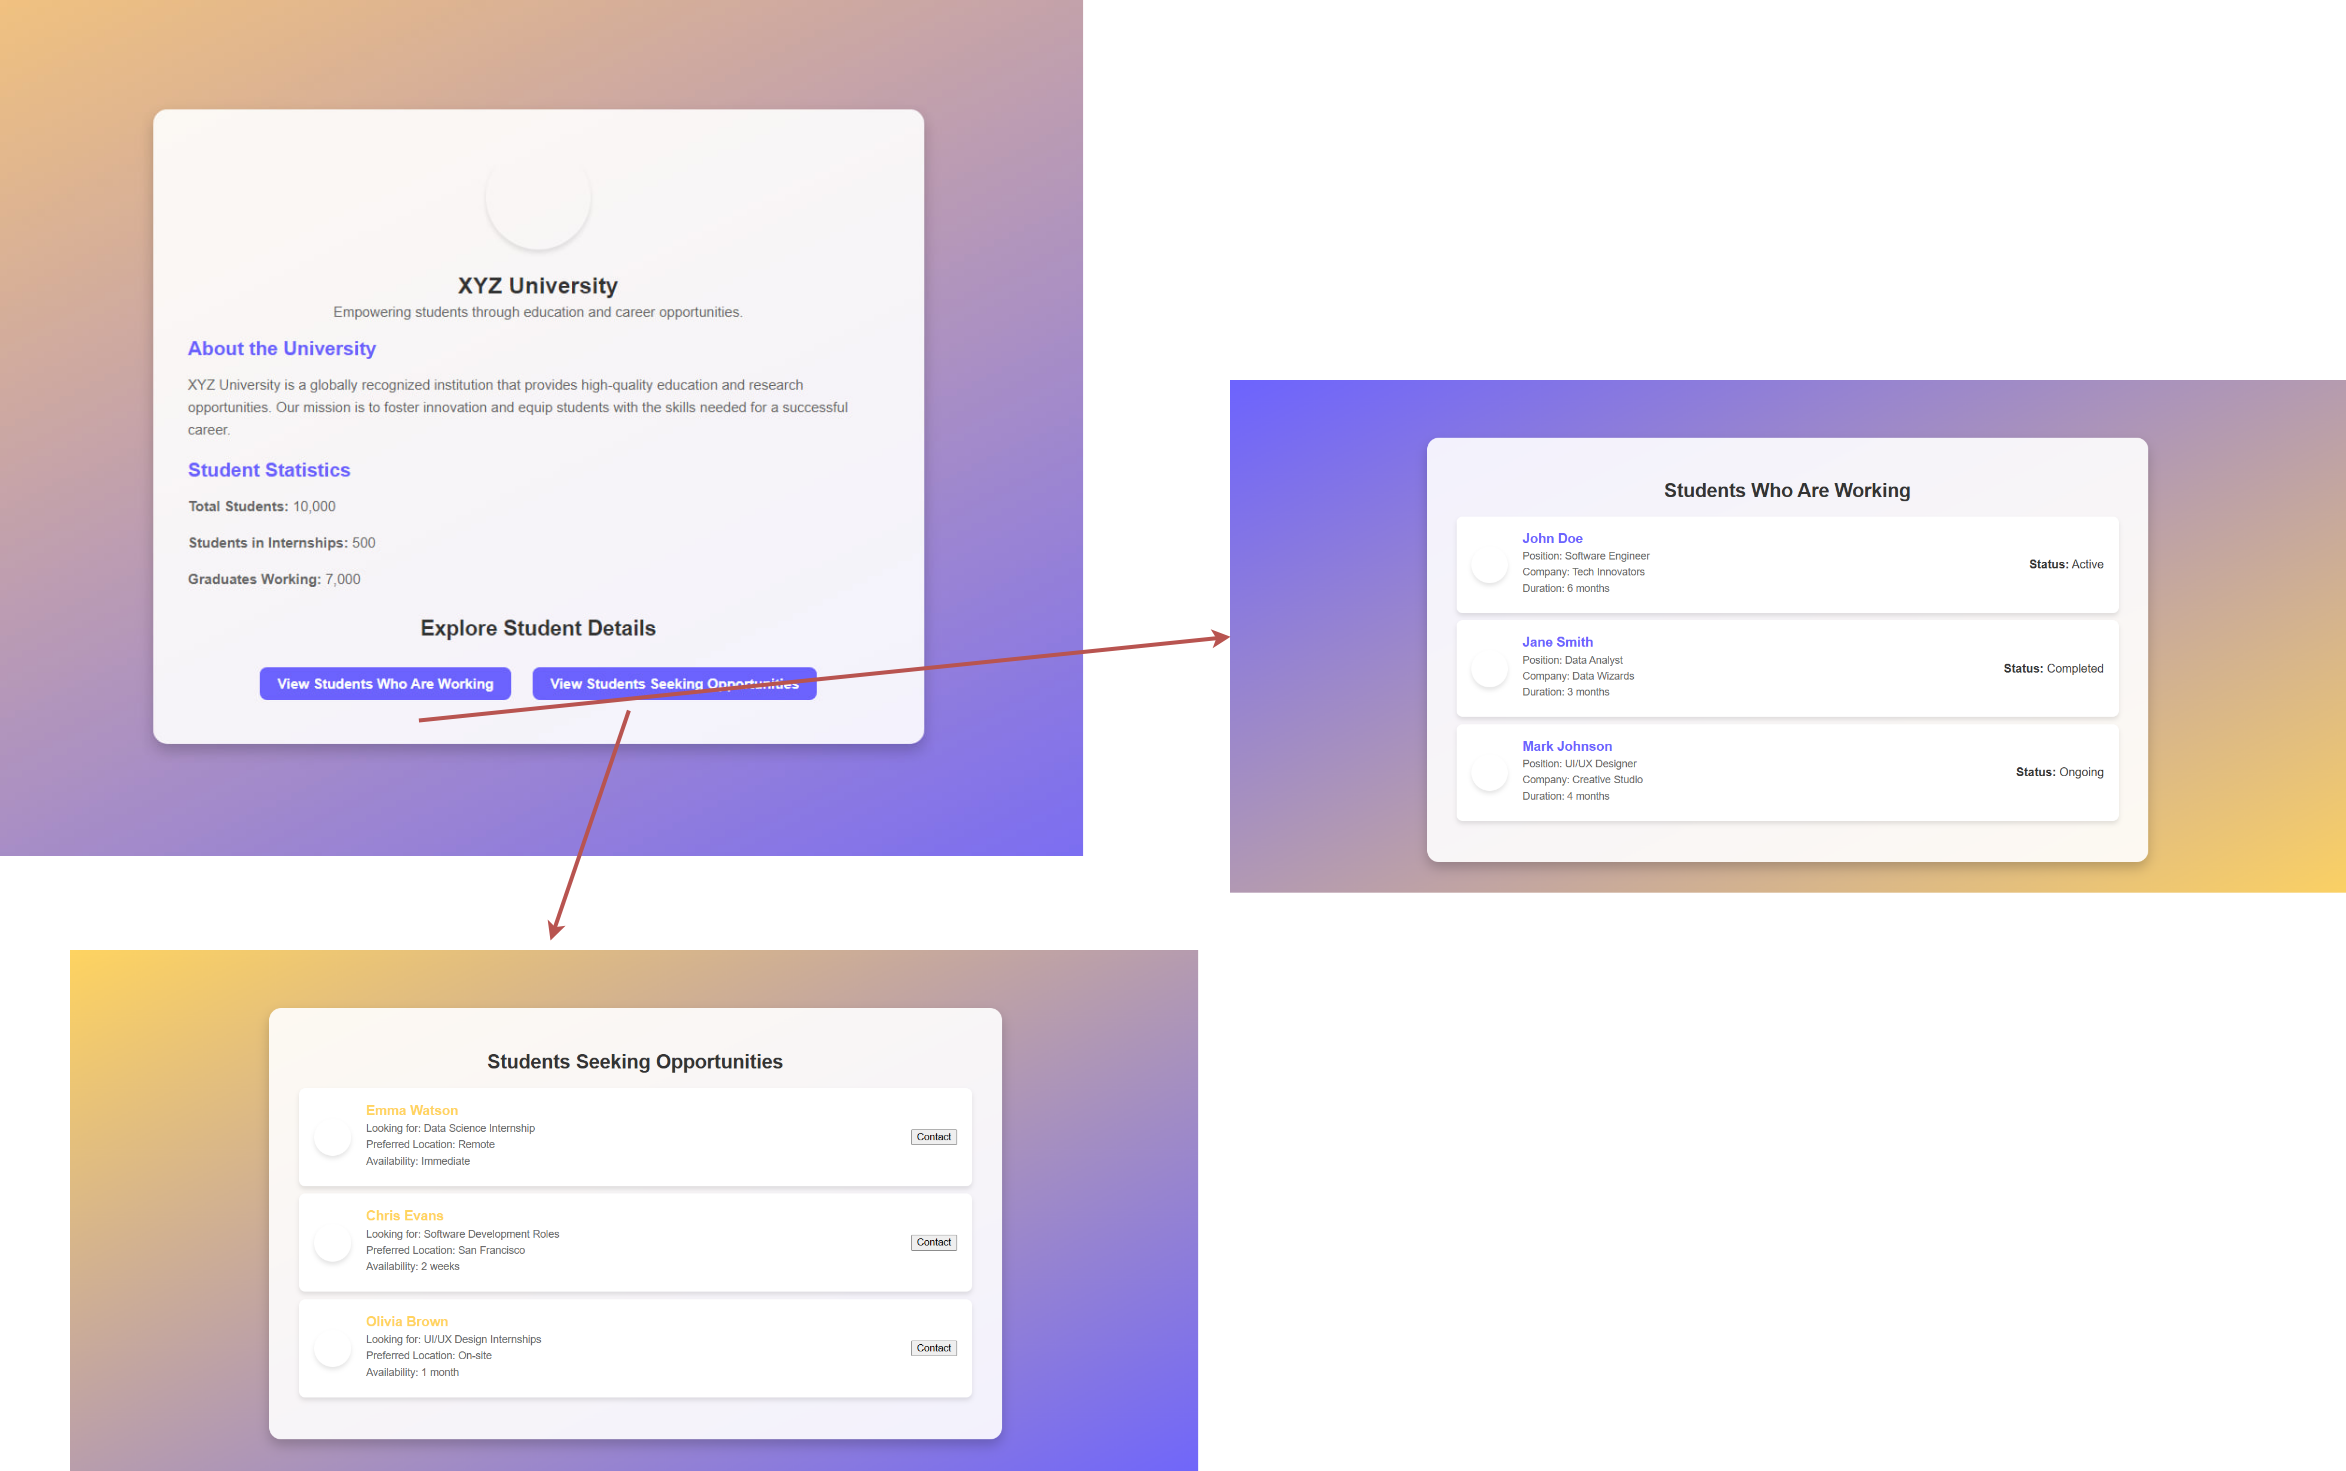
\includegraphics[width=0.9\textwidth, angle=0]{Images/Main3.png}
\caption{\label{fig:metamodel}University Dashboard Navigation: The interface allows universities to view statistics and access detailed lists of students who are currently working or seeking opportunities, helping administrators manage student engagement efficiently.}
\end{figure}

\begin{figure}[!h]
\centering
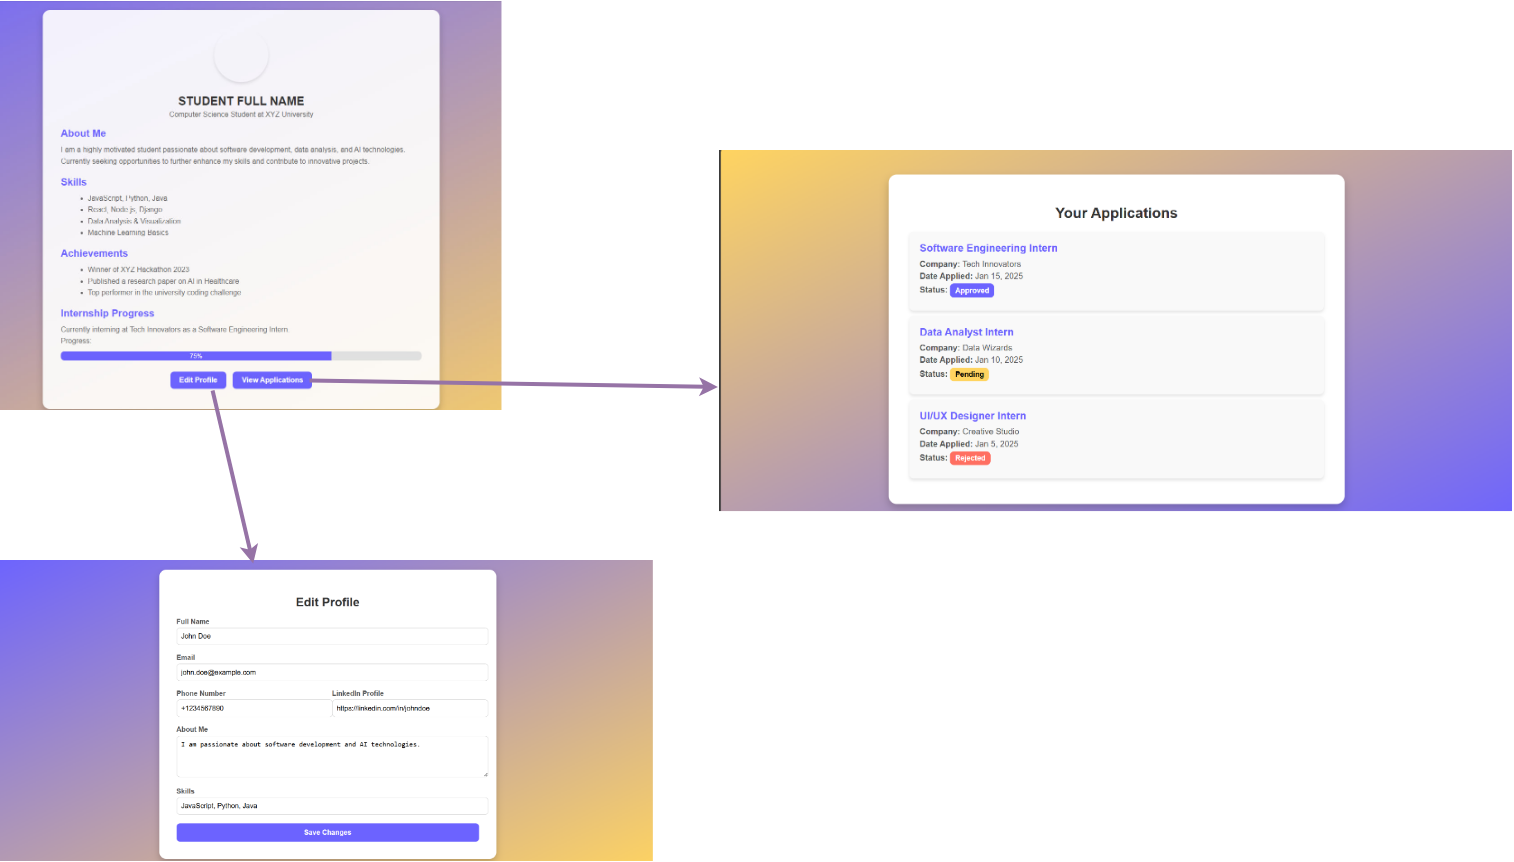
\includegraphics[width=0.9\textwidth, angle=0]{Images/Main4.png}
\caption{\label{fig:metamodel}Student Profile and Actions: A comprehensive student profile dashboard displaying skills, achievements, and internship progress. The navigation includes options to edit personal information and view detailed application statuses.}
\end{figure}

\begin{figure}[!h]
\centering
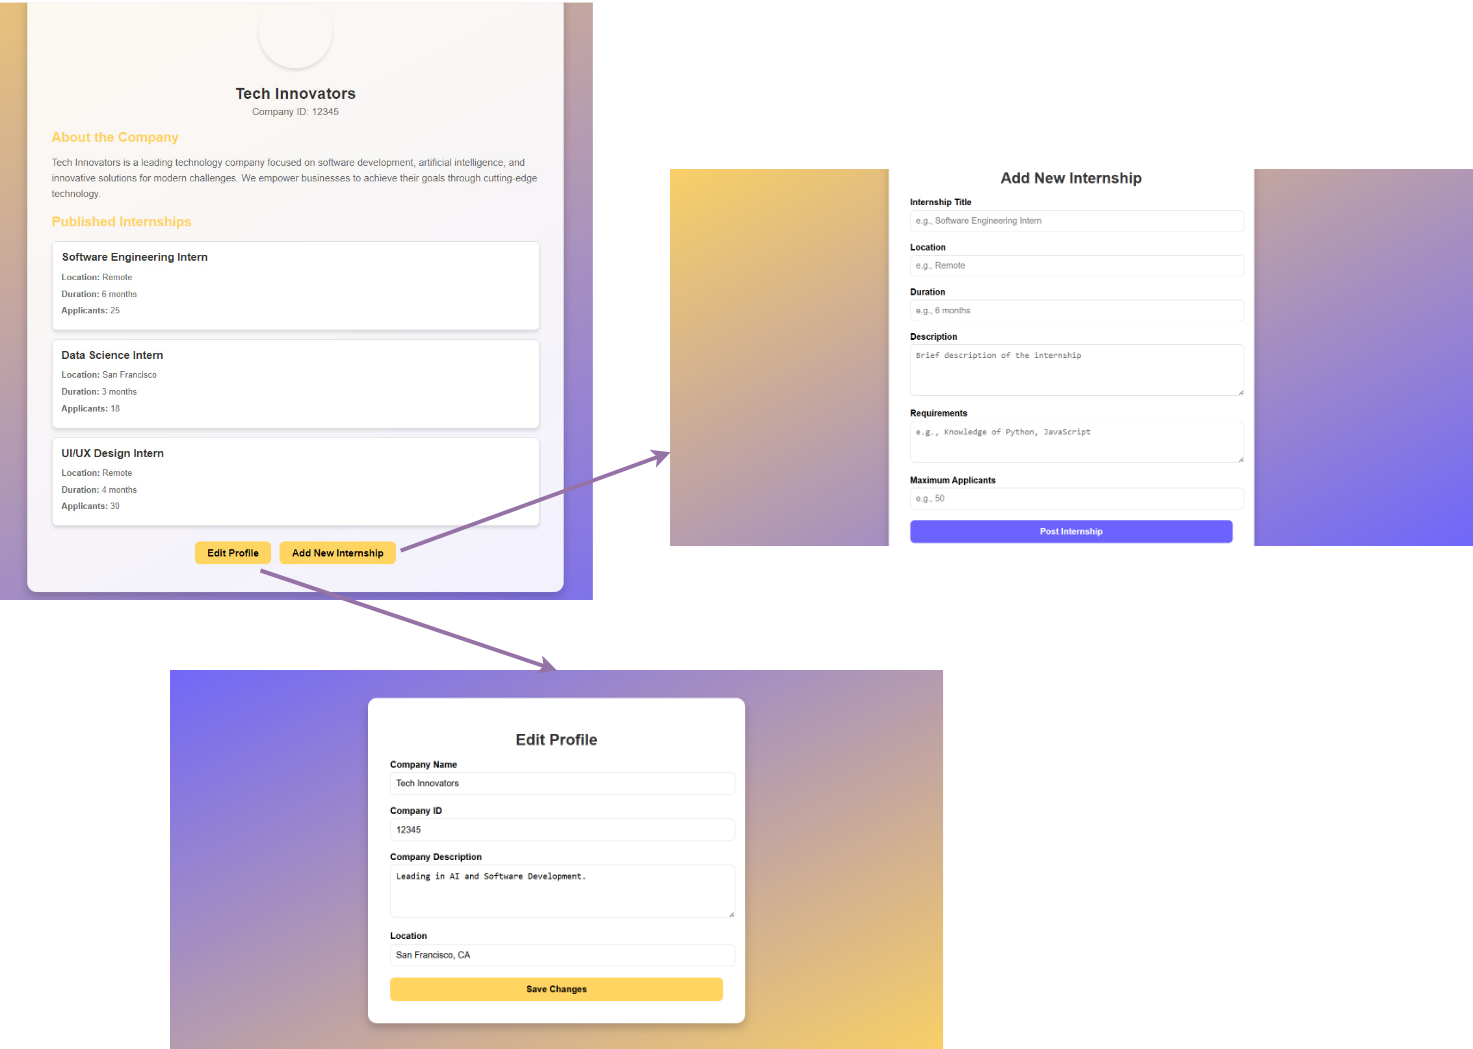
\includegraphics[width=0.9\textwidth, angle=0]{Images/Main5.png}
\caption{\label{fig:metamodel}Company Profile and Management: An interface for company representatives to manage their profiles and internship offerings. Includes options to edit company details and add new internships with customizable parameters.}
\end{figure}

 

%------------------------------------------------------------------------------------------------------------------------------------------------
\clearpage
{\color{Blue}{\section{Requirement traceability}}}
\label{sect:rectrace}
\begin{table}[h!]
\centering
\begin{tabular}{|l|p{10cm}|}
\hline
\textbf{Requirements} & 
[R1] The S\&C system allows new users (students, universities, and companies) to register by giving
 their credentials (e.g., name, email address, password).\\
\hline
\textbf{Components} & 
\begin{itemize}
    \item Database (Stores user information securely)
    \item Profile Manager (Handles user profile creation and updates)
    \item Authenticate Manager (Manages user authentication and credentials)
    \item Notification Manager (Sends confirmation email after registration)
\end{itemize} \\
\hline
\end{tabular}
\label{tab:req_comp}
\end{table}

\begin{table}[h!]
\centering
\begin{tabular}{|l|p{10cm}|}
\hline
\textbf{Requirements} & 
[R2] The system allows users (students, universities, and companies) to login.\\
\hline
\textbf{Components} & 
\begin{itemize}
    \item Database (Verifies credentials against stored data)
    \item Profile Manager (Manages user session after login)
    \item Authenticate Manager (Validates user credentials and manages sessions)
    \item Notification Manager (Notifies users of successful login or errors)
\end{itemize} \\
\hline
\end{tabular}
\label{tab:req_comp}
\end{table}

\begin{table}[h!]
\centering
\begin{tabular}{|l|p{10cm}|}
\hline
\textbf{Requirements} & 
[R3] The system allows students to create and update their profile (experience, skills, CV).\\
\hline
\textbf{Components} & 
\begin{itemize}
    \item Database (Stores student profile data such as skills, experience, and CV)
    \item Profile Manager (Handles student profile creation and updates)
    \item Recommendation Engine (Provides feedback to students about profile completeness)
\end{itemize} \\
\hline
\end{tabular}
\label{tab:req_comp}
\end{table}

\begin{table}[h!]
\centering
\begin{tabular}{|l|p{10cm}|}
\hline
\textbf{Requirements} & 
[R4] The system allows companies to create and update company’s profile (about, field of work, achievements).\\
\hline
\textbf{Components} & 
\begin{itemize}
    \item Database (Stores company details and achievements)
    \item Profile Manager (Manages company profile data)
    \item Company Portal (Provides interface for companies to manage their profiles)
\end{itemize} \\
\hline
\end{tabular}
\label{tab:req_comp}
\end{table}

\begin{table}[h!]
\centering
\begin{tabular}{|l|p{10cm}|}
\hline
\textbf{Requirements} & 
[R5] The system allows universities to create and update their profile.\\
\hline
\textbf{Components} & 
\begin{itemize}
    \item Database (Stores university profile information)
    \item Profile Manager (Manages university data)
    \item University Admin Portal (Provides interface for universities to manage their profiles)
\end{itemize} \\
\hline
\end{tabular}
\label{tab:req_comp}
\end{table}

\begin{table}[h!]
\centering
\begin{tabular}{|l|p{10cm}|}
\hline
\textbf{Requirements} & 
[R6] The system helps students in creating their CVs by giving intelligent suggestions for making a stronger CV and pointing out mistakes.\\
\hline
\textbf{Components} & 
\begin{itemize}
    \item Database (Stores CV data)
    \item Profile Manager (Integrates feedback with user profiles)
    \item Recommendation Engine (Provides intelligent suggestions based on user input)
    \item Recommendation Engine (Analyzes user data for profile improvement)
\end{itemize} \\
\hline
\end{tabular}
\label{tab:req_comp}
\end{table}

\begin{table}[h!]
\centering
\begin{tabular}{|l|p{10cm}|}
\hline
\textbf{Requirements} & 
[R7] Students can search for internship opportunities by clicking on the "Search" button.\\
\hline
\textbf{Components} & 
\begin{itemize}
    \item Database (Stores internship data)
    \item Search Engine (Handles internship searches)
    \item Recommendation Engine (Suggests internships based on student profiles)
    \item Notification Manager (Notifies students of available internships)
\end{itemize} \\
\hline
\end{tabular}
\label{tab:req_comp}
\end{table}

\begin{table}[h!]
\centering
\begin{tabular}{|l|p{10cm}|}
\hline
\textbf{Requirements} & 
[R8] Students can apply to the desired internship by clicking on the "Apply" button for an internship post.\\
\hline
\textbf{Components} & 
\begin{itemize}
    \item Database (Stores submitted applications)
    \item Profile Manager (Tracks application status)
    \item Notification Manager (Notifies companies about new applications)
\end{itemize} \\
\hline
\end{tabular}
\label{tab:req_comp}
\end{table}

\begin{table}[h!]
\centering
\begin{tabular}{|l|p{10cm}|}
\hline
\textbf{Requirements} & 
[R9] The system provides personalized recommendations to the students for internships based on students' profiles and skills which match with available internships.\\
\hline
\textbf{Components} & 
\begin{itemize}
    \item Database (Stores internship listings and student profiles)
    \item Recommendation Engine (Handles recommendation logic)
    \item Notification Manager (Alerts students about recommended internships)
\end{itemize} \\
\hline
\end{tabular}
\label{tab:req_comp}
\end{table}

\begin{table}[h!]
\centering
\begin{tabular}{|l|p{10cm}|}
\hline
\textbf{Requirements} & 
[R10] Students can automatically apply to any recommended internship by clicking on the "Accept" button.\\
\hline
\textbf{Components} & 
\begin{itemize}
    \item Database (Stores auto-applied internship data)
    \item Profile Manager (Updates user application status)
    \item Recommendation Engine (For getting the matched internships)
    \item Notification Manager (Alerts users of successful application)
\end{itemize} \\
\hline
\end{tabular}
\label{tab:req_comp}
\end{table}

\begin{table}[h!]
\centering
\begin{tabular}{|l|p{10cm}|}
\hline
\textbf{Requirements} & 
[R11] Companies can post internship opportunities and descriptions which include application domain, tasks to be performed, skills required.\\
\hline
\textbf{Components} & 
\begin{itemize}
    \item Database (Stores internship listings)
    \item Company Portal (Provides interface for companies to post internships)
    \item Profile Manager (For posting internship description)
    \item Notification Manager (Notifies users of new internship postings)
\end{itemize} \\
\hline
\end{tabular}
\label{tab:req_comp}
\end{table}

\begin{table}[h!]
\centering
\begin{tabular}{|l|p{10cm}|}
\hline
\textbf{Requirements} & 
[R12] The system can provide recommendations to improve the internship posts by companies.\\
\hline
\textbf{Components} & 
\begin{itemize}
    \item Database (Stores internship descriptions and related data)
    \item Recommendation Engine (Analyzes internship posts and suggests improvements)
    \item \textbf Recommendation Engine (Provides suggestions for improvement)
\end{itemize} \\
\hline
\end{tabular}
\label{tab:req_comp}
\end{table}

\begin{table}[h!]
\centering
\begin{tabular}{|l|p{10cm}|}
\hline
\textbf{Requirements} & 
[R13] The companies can prepare a questionnaire in the system to be forwarded to the students to get
additional information from them when the selection process starts.\\
\hline
\textbf{Components} & 
\begin{itemize}
    \item Company Portal (Provides an interface for companies to create questionnaires)
    \item Profile Manager (Handles student and company profile management)
    \item Database (Stores questionnaire data and responses)
    \item Notification Manager (Notifies students about questionnaire assignments)
\end{itemize} \\
\hline
\end{tabular}
\label{tab:req_comp}
\end{table}

\begin{table}[h!]
\centering
\begin{tabular}{|l|p{10cm}|}
\hline
\textbf{Requirements} & 
[R14] The system can recommend companies about available students who match the job description and skills by applying statistical analysis based on the characteristics of students and internships.\\
\hline
\textbf{Components} & 
\begin{itemize}
    \item Recommendation Engine (Handles matching students with internships based on their profiles)
    \item Profile Manager (Manages student and company profiles)
    \item Database (Stores student, company, and internship data for analysis)
    \item Notification Manager (Notifies companies about matching students)
\end{itemize} \\
\hline
\end{tabular}
\label{tab:req_comp}
\end{table}

\begin{table}[h!]
\centering
\begin{tabular}{|l|p{10cm}|}
\hline
\textbf{Requirements} & 
[R15] The system notifies students and companies once every day to recommend new matches.\\
\hline
\textbf{Components} & 
\begin{itemize}
    \item Notification Manager (Manages daily notifications about new matches)
    \item Recommendation Engine (Suggests new matches)
    \item Database (Stores match history and user preferences)
\end{itemize} \\
\hline
\end{tabular}
\label{tab:req_comp}
\end{table}

\begin{table}[h!]
\centering
\begin{tabular}{|l|p{10cm}|}
\hline
\textbf{Requirements} & 
[R16] Companies can track applications and review candidate CVs.\\
\hline
\textbf{Components} & 
\begin{itemize}
    \item Company Portal (Displays applications and CVs for review)
    \item Database (Stores applications and CVs)
    \item Profile Manager (Handles the management of student profiles)
\end{itemize} \\
\hline
\end{tabular}
\label{tab:req_comp}
\end{table}

\begin{table}[h!]
\centering
\begin{tabular}{|l|p{10cm}|}
\hline
\textbf{Requirements} & 
[R17] Companies can accept or reject an application or a suggestion by the system by clicking on "Accept" or "Reject" buttons for each application.\\
\hline
\textbf{Components} & 
\begin{itemize}
    \item Company Portal (Provides accept/reject functionality for applications)
    \item Selection Process (Manages the acceptance/rejection process)
    \item Database (Stores the updated status of applications)
    \item Notification Manager (Notifies students of acceptance/rejection)
\end{itemize} \\
\hline
\end{tabular}
\label{tab:req_comp}
\end{table}

\begin{table}[h!]
\centering
\begin{tabular}{|l|p{10cm}|}
\hline
\textbf{Requirements} & 
[R18] A messaging channel is opened when a recommendation is accepted by both student and company or an application by student is accepted by company.\\
\hline
\textbf{Components} & 
\begin{itemize}
    \item Student Portal (Provides interface for messaging students)
    \item Company Portal (Provides interface for messaging companies)
    \item Selection Process (Manages messaging after acceptance)
    \item Database (Stores message history)
    \item Notification Manager (Notifies both students and companies of new messages)
\end{itemize} \\
\hline
\end{tabular}
\label{tab:req_comp}
\end{table}

\begin{table}[h!]
\centering
\begin{tabular}{|l|p{10cm}|}
\hline
\textbf{Requirements} & 
[R19] The prepared questionnaire is forwarded to the student.\\
\hline
\textbf{Components} & 
\begin{itemize}
    \item Student Portal (Displays questionnaire to students)
    \item Database (Stores student responses to questionnaires)
    \item Notification Manager (Notifies students about new questionnaires)
\end{itemize} \\
\hline
\end{tabular}
\label{tab:req_comp}
\end{table}

\begin{table}[h!]
\centering
\begin{tabular}{|l|p{10cm}|}
\hline
\textbf{Requirements} & 
[R20] The system helps in the management of the selection process by scheduling interviews.\\
\hline
\textbf{Components} & 
\begin{itemize}
    \item Selection Process (Manages interview scheduling)
    \item University Admin Portal (Manages scheduling of university-administered interviews)
    \item Notification Manager (Notifies both student and company about scheduled interviews)
    \item Database (Stores interview scheduling data)
\end{itemize} \\
\hline
\end{tabular}
\label{tab:req_comp}
\end{table}

\begin{table}[h!]
\centering
\begin{tabular}{|l|p{10cm}|}
\hline
\textbf{Requirements} & 
[R21] The system sends interview link or interview location to both student and company.\\
\hline
\textbf{Components} & 
\begin{itemize}
    \item Selection Process (Provides interview link and location data)
    \item Database (Stores interview details and links)
    \item Notification Manager (Notifies both student and company)
    \item Email Service (Sends interview details via email)
\end{itemize} \\
\hline
\end{tabular}
\label{tab:req_comp}
\end{table}

\begin{table}[h!]
\centering
\begin{tabular}{|l|p{10cm}|}
\hline
\textbf{Requirements} & 
[R22] The system allows the company to update the interview results.\\
\hline
\textbf{Components} & 
\begin{itemize}
    \item Company Portal (Provides an interface to update interview results)
    \item Selection Process (Stores and processes interview results)
    \item Database (Stores interview results)
    \item Notification Manager (Notifies students about interview results)
\end{itemize} \\
\hline
\end{tabular}
\label{tab:req_comp}
\end{table}

\begin{table}[h!]
\centering
\begin{tabular}{|l|p{10cm}|}
\hline
\textbf{Requirements} & 
[R23] Interview results are updated in the platform and users are notified.\\
\hline
\textbf{Components} & 
\begin{itemize}
    \item Selection Process (Handles interview result updating)
    \item Notification Manager (Sends interview result notifications)
    \item Database (Stores updated results)
\end{itemize} \\
\hline
\end{tabular}
\label{tab:req_comp}
\end{table}

\begin{table}[h!]
\centering
\begin{tabular}{|l|p{10cm}|}
\hline
\textbf{Requirements} & 
[R24] The system collects feedback from students and companies to then use the gathered data to better its analysis and recommendation algorithm.\\
\hline
\textbf{Components} & 
\begin{itemize}
    \item Feedback \& Analytics (Processes collected feedback)
    \item Recommendation Engine (Uses feedback for improvements)
    \item Database (Stores feedback data)
    \item Notification Manager (Notifies users about feedback requests)
    \item Feedback \& Analytics (For improving the recommendation model)
\end{itemize} \\
\hline
\end{tabular}
\label{tab:req_comp}
\end{table}

\begin{table}[h!]
\centering
\begin{tabular}{|l|p{10cm}|}
\hline
\textbf{Requirements} & 
[R25] The system has a dedicated page to keep track and monitor all the ongoing search and selection processes for all three types of users (students, university, companies).\\
\hline
\textbf{Components} & 
\begin{itemize}
    \item User Interfaces
    \item Internship Monitor Engine (Monitors the overall status of selection)
    \item Database (Stores real-time data of ongoing processes)
\end{itemize} \\
\hline
\end{tabular}
\label{tab:req_comp}
\end{table}

\begin{table}[h!]
\centering
\begin{tabular}{|l|p{10cm}|}
\hline
\textbf{Requirements} & 
[R26] During the selection process and during the interview the involved parties can raise concerns or complaints which will be monitored by the university.\\
\hline
\textbf{Components} & 
\begin{itemize}
    \item Complaint Manager (Manages complaint submission and tracking)
    \item University Admin Portal (Monitors and resolves complaints)
    \item Notification Manager (Notifies concerned parties about complaints)
    \item Database (Stores complaint data)
\end{itemize} \\
\hline
\end{tabular}
\label{tab:req_comp}
\end{table}

\begin{table}[h!]
\centering
\begin{tabular}{|l|p{10cm}|}
\hline
\textbf{Requirements} & 
[R27] The system allows the university to decide on required actions to perform like warning to respective parties or interruption of internship and updates the same on the platform.\\
\hline
\textbf{Components} & 
\begin{itemize}
    \item University Admin Portal (Manages actions and decisions)
    \item Notification Manager (Notifies concerned parties about actions)
    \item Database (Stores decision data and actions)
\end{itemize} \\
\hline
\end{tabular}
\label{tab:req_comp}
\end{table}













%------------------------------------------------------------------------------------------------------------------------------------------------
\clearpage
{\color{Blue}{\section{Implementation, Integration and Test Plan}}}
\label{sect:implementation-test}
\subsection{Implementation Plan}

The implementation plan defines the sequential steps for developing the system's components, ensuring that each feature and module is designed, developed, and tested effectively. The Bottom-Up methodology will be used to break down the entire system into simplest possible subsystems that recursively build up to the required solution. Each component will follow the Single Responsibility Principle (SRP) and will be implemented using Test-Driven Development (TDD).

\subsubsection{Development of Core Components}

\paragraph{User Authentication and Profile Management:}
The objective is to implement secure registration and login functionalities for students, companies, and universities, with each user type having their own profile and corresponding data. To achieve this, we will develop the user registration functionality, allowing for input of name, email, password, and role selection. We will also implement login and session management to ensure secure access. Each user type will be able to create and edit their profile, with students entering their academic and experience details, while companies provide internship descriptions. For this, we will use OAuth 2.0 for secure authentication and PostgreSQL/MySQL for storing user data.

\begin{figure}[H]
\centering
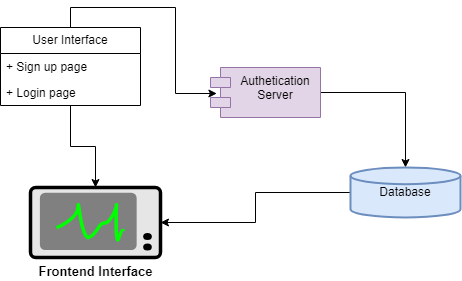
\includegraphics[width=0.8\textwidth]{Images/core1.png}
\caption{User Authentication and Profile Management.}
\end{figure}

\paragraph{Internship Search and Application System:}
The objective of this component is to provide students with a way to search for, view, and apply for internships. This will involve developing a search functionality that uses filters like location, skills, and internship type. The system will display relevant internship details such as job descriptions, company names, and locations. Students will also have the option to apply directly to internships by clicking the "Apply" button. Elasticsearch will be used to index and search internship listings, and we will integrate this functionality with the backend API to display search results in real-time.

\begin{figure}[H]
\centering
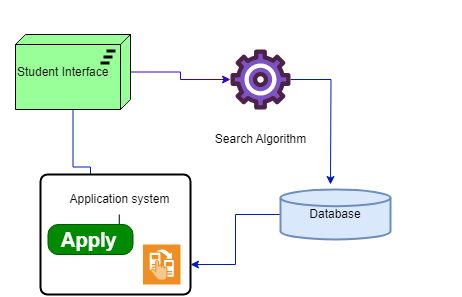
\includegraphics[width=0.8\textwidth]{Images/core2.png}
\caption{Internship Search and Application System.}
\end{figure}

\paragraph{Internship Posting:}
Companies will be able to post internships, and the system will automatically match students with relevant positions based on their profiles. To implement this, we will create the "Post Internship" functionality, which will allow companies to add internship roles. The frontend for posting the internship details will show writing improvement suggestions to the author to increase the likelihood of finding suitable matches with Student profiles. The backend service will be developed using Node.js.
The system will use the Recommendation Engine described below to recommend internships to students, based on their profile data, such as skills, experience, and location preferences.

\paragraph{Recommendation/Matching Engine:}
 The Recommendation/Matching Engine will run as a Cron Job at regular intervals of 24 hours for each Student to identify Internships relevant to their skills and background. In order to achieve performance optimization, an Embedding will be calculated ahead-of-time for each Student profile using a Neural Network trained on anonymized data of past Student profile and Internship matches. The Neural Network will use Matrix Factorization to learn the representation of Latent Factors from the available profile and internship attributes and create the Embedding. This Embedding will be re-calculated whenever a Student updates any attributes of their profile. The Recommendation/Matching Engine will use a Model-Based Collaborative Filtering (MCBF) to match new Student profiles to Internships based on the pre-calculated Embeddings to optimize compute resource utilization. The system will use the Notification Manager to alert both students and companies about new matches. The backend logic will be developed using Python, and machine learning algorithms will be applied for the matching process.

\begin{figure}[H]
\centering
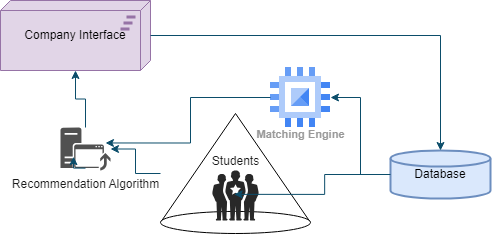
\includegraphics[width=0.8\textwidth]{Images/core3.png}
\caption{Internship Posting and Matching Engine.}
\end{figure}

\paragraph{Interview Scheduling and Feedback Collection:}
The system will support companies in scheduling interviews with selected candidates and collecting feedback after the interview. The interview scheduling tool will allow students and companies to select available time slots. Integration with a video conferencing system like Zoom will allow for virtual interviews, and the system will also collect feedback after each interview. For scheduling, we will use the Google Calendar API, and Zoom will be integrated for video calls. The feedback system will be custom-built to collect and store feedback from both students and companies.

\begin{figure}[H]
\centering
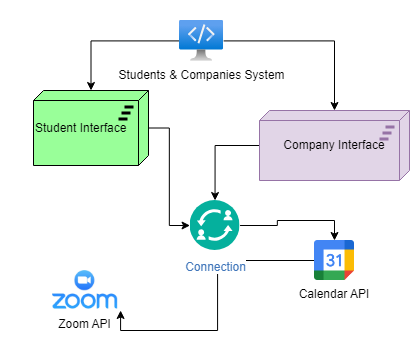
\includegraphics[width=0.8\textwidth]{Images/core42.png}
\caption{Interview Scheduling.}
\end{figure}
\begin{figure}[H]
\centering
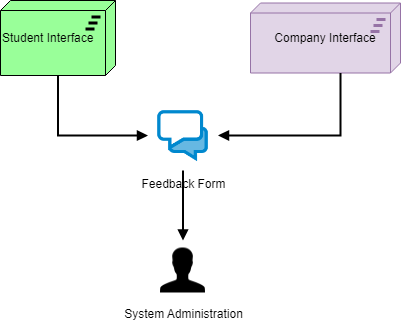
\includegraphics[width=0.8\textwidth]{Images/core41.png}
\caption{Feedback Collection.}
\end{figure}

\paragraph{Complaint Handling and University Monitoring System:}
This component will enable universities to monitor student internship progress and handle complaints from both students and companies. Universities will be able to track the status of all students' internship applications using a dedicated dashboard. A complaint reporting and resolution workflow will be developed to allow students and companies to raise and resolve issues. Notifications will be sent to the involved parties (students, companies, universities), and the university will oversee the resolution process. The notification system will be built using email or push notifications, and the interface for universities will be user-friendly and easily accessible.

\begin{figure}[H]
\centering
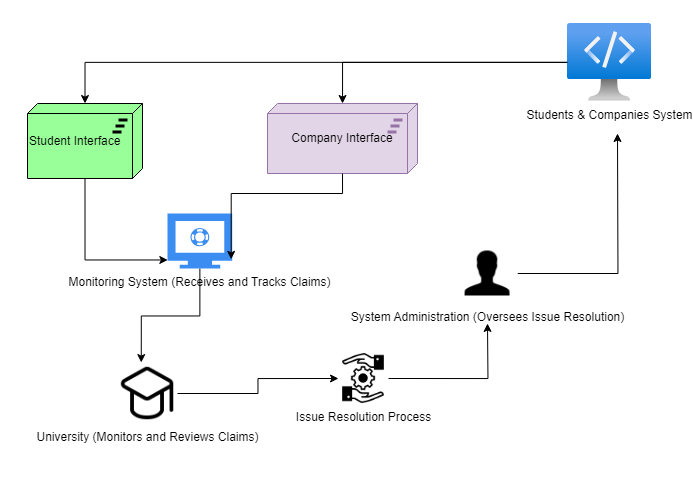
\includegraphics[width=0.8\textwidth]{Images/core5.png}
\caption{Complaint Handling and University Monitoring System.}
\end{figure}

\subsubsection{Technology Stack}

\begin{itemize}
    \item \textbf{Frontend:} ReactJS or Angular will be used to build responsive and interactive user interfaces.
    \item \textbf{Backend:} Node.js with Express.js or Django will handle business logic and REST API services.
    \item \textbf{Database:} PostgreSQL or MySQL will store structured data such as user profiles, internship listings, and applications.
    \item \textbf{Search Engine:} Elasticsearch will be used for indexing and filtering internship listings efficiently.
    \item \textbf{Recommendation System:} Python or JavaScript-based machine learning models will be used for matching students with internships.
    \item \textbf{Video Conferencing:} Zoom API will be integrated for virtual interviews.
    \item \textbf{Notification System:} Email services like NodeMailer or SendGrid will be used for sending user notifications.
\end{itemize}

\subsection{Integration Plan}

Once the core components are developed, we will proceed with the integration phase. This phase involves combining the various subsystems, ensuring smooth data flow, and confirming that all functionalities work together.

\subsubsection{Integration of User Authentication and Profile Management}
The user authentication system will be integrated with the frontend, allowing users to sign up, log in, and access their profile pages. Role-based views (Student, Company, University) will be displayed based on the user’s role.

\subsubsection{Integration of Internship Search and Application System}
The search functionality will be connected to the backend to fetch real-time data, and the "Apply" functionality will be integrated to submit student applications to companies.

\subsubsection{Integration of Internship Posting and Matching Engine}
Companies will be able to post internships, and the system will match these postings with student profiles. The matching engine will use the student’s profile data to recommend internships, and notifications will inform both students and companies about new matches.

\subsubsection{Integration of Interview Scheduling and Feedback Collection}
The interview scheduling feature will be integrated, allowing both students and companies to select available time slots. Zoom integration will ensure video meetings, and feedback will be collected and stored after interviews.

\subsubsection{Integration of Complaint Handling and University Monitoring}
Universities will be able to monitor the internship status of students and resolve complaints through the system. The complaint submission and resolution process will be integrated, and notifications will inform all relevant parties.

\subsubsection{End-to-End Testing}
We will ensure that data flows seamlessly between the frontend, backend, and database. Additionally, we will test for any UI/UX issues and resolve any discrepancies. Unit tests for individual components and integration tests for interactions between modules will be conducted.

\subsection{Testing Plan}

Testing will be done iteratively during development, followed by extensive system testing to ensure robustness and correctness.

\subsubsection{Unit Testing}
The goal is to verify that individual components, such as user authentication, profile creation, internship search, matching algorithm, and interview scheduling, work correctly.

\subsubsection{Integration Testing}
We will verify that the components work together seamlessly. For example, we will check if user registration leads to successful login and profile creation, if students can apply for internships, and if the matching system works as intended.

\subsubsection{Functional Testing}
This type of testing will ensure that the system meets all functional requirements. Students should be able to search for internships, companies should be able to post internships, and universities should be able to monitor student progress and handle complaints.

\subsubsection{Performance Testing}
We will conduct load testing to simulate multiple users accessing the system simultaneously. We will also test the system’s response time and performance under peak usage conditions.

\subsubsection{Security Testing}
The security of the platform will be tested to ensure that user credentials are encrypted, and the system is protected against common security threats such as SQL injection and XSS attacks.

\subsubsection{Technology Stack}

\begin{itemize}
    \item \textbf{Testing Tools:} Jest or Mocha for unit testing the individual components of the system.
    \item \textbf{Integration Testing Tools:} Postman or Supertest for testing REST API integrations between frontend and backend.
    \item \textbf{Performance Testing:} Apache JMeter or LoadRunner for conducting load and performance tests.
    \item \textbf{Security Testing:} OWASP ZAP or Burp Suite for vulnerability scanning and security testing.
\end{itemize}

\subsubsection{User Acceptance Testing (UAT)}
Actual users (students, companies, universities) will test the system to ensure it meets their needs. Feedback will be collected, and any necessary adjustments will be made before deployment.


%------------------------------------------------------------------------------------------------------------------------------------------------
\clearpage
{\color{Blue}{\section{Effort Spent}}}
\label{sect:effort}
This section shows the amount of time that each member has spent to produce the document. Please notice that each unit is the result of coordinated work among all the members.

\begin{table}[h]
\centering
\begin{tabularx}{\textwidth}{| X | X | X |}
\hline
\textbf{UNIT} & \textbf{MEMBERS} & \textbf{HOURS} \\ [1ex]
\hline
Section 1 &  S. Chaudhury   & 3h \\ [1ex]
\hline
Section 2.1 &  S. Chaudhury  & 2h \\ [1ex]
\hline
Section 2.2 &  D. Motiallah  & 2h \\ [1ex]
\hline
Section 2.3  &  S. Chaudhury  & 3h \\ [1ex]
\hline
\text{Section 2.4 \newline(Sequence diagrams)} &  D. Motiallah \& S. Chaudhury   & 16h \\ [1ex]
\hline
\text{Section 2.4 (Sequence diagrams descriptions)} &  S. Chaudhury   & 5 h \\ [1ex]
\hline
Section 2.5  &  D. Motiallah  & 6h \\ [1ex]
\hline
Section 2.6 \& 2.7 &  D. Motiallah \& S. Chaudhury   & 4h \\ [1ex]
\hline
Section 3 &  D.Islam  & 12h \\ [1ex]
\hline
Section 4 &  D.Islam  & 7h \\ [1ex]
\hline
Section 5 &  D.Islam, S. Chaudhury  & 13h \\ [1ex]
\hline
Redaction &  S. Chaudhury  & 5h \\ [1ex]
\hline
\end{tabularx}
\end{table}


\clearpage
\section{\color{Blue}{References and Tools}}

\begin{enumerate}
    \item GitHub: https://www.github.com
    \item GitHub Actions: https://github.com/features/actions
    \item The UI have been made with:
    \begin{itemize}
    \item JavaScript documentation:https://developer.mozilla.org/en-US/docs/Web/JavaScript 
    \item Node.js documentation: https://nodejs.org/api/all.html
    \item HTML documentation: https://html.spec.whatwg.org/
    \item Bootstrap CSS framework: https://getbootstrap.com/docs/5.3/getting-started/introduction/
    \end{itemize}
   
    \item Zoom API: https://developers.zoom.us/docs/api/
    \item Calendar API: https://developers.google.com/calendar/api/guides/overview?hl=ru
    \item Diagrams have been made with draw.io: https://app.diagrams.net/ 
   
\end{enumerate}

%------------------------------------------------------------------------------------------------------------------------------------------------

% \clearpage
% \addcontentsline{toc}{section}{References}
% \bibliographystyle{plain}
% \bibliography{main}
%------------------------------------------------------------------------------------------------------------------------------------------------

\end{document}
